\documentclass[12pt]{article}
\usepackage{sbc-template}
\usepackage{graphicx,url}
\usepackage[brazil]{babel}   
\usepackage[utf8]{inputenc}
\usepackage{graphicx}
\usepackage{subfigure}
\usepackage{amsmath}
\usepackage{bbm}
\usepackage{cite}
\usepackage{listings}
\usepackage{color}
\usepackage{indentfirst}
\usepackage{float}
\usepackage{dirtree}

\lstset{language=Python,
                basicstyle=\ttfamily,
                keywordstyle=\color{blue}\ttfamily,
                stringstyle=\color{red}\ttfamily,
                commentstyle=\color{green}\ttfamily,
                morecomment=[l][\color{magenta}]{\#}
}


\title{Visualização de Dados de Informações Extraídas da Web - Um Estudo sobre Conteúdo Popular Japonês}
\author{Gabriel Fontenelle Senno Silva\inst{1}}
\address 
{Centro Universitário Senac - Campus Santo Amaro
  (SENAC-SP)\\
  Av. Engenheiro Eusébio Stevaux, 823 -- São Paulo -- CEP 04696-000 -- SP -- Brasil
%\nextinstitute
%  Departamento de Tecnologia da Informação\\
%  Bacharelado em Ciência da Computação
  \email{{colecionador.gabriel@gmail.com}}
}

\begin{document} 
\maketitle

\begin{resumo} 

Primeiramente falamos sobre alguns dos conteúdos pertencentes a cultura popular japonesa e apresentamos os websites utilizados para extração de conteúdo, depois apresentamos em detalhes a modelagem do banco de dados, discutimos a implementação do crawler e o desenvolvimento de visualizações de dados e por fim mostramos as visualizações produzidas.

\end{resumo}


\section{Introdução}

Visualização de dados é uma forma de comunicar visualmente informações, com base em um conjunto de dados, que de outra forma não seriam facilmente identificáveis.

O foco deste trabalho é a criação de visualizações a partir de dados extraídos de websites que disponibilizam quantidade maciça de conteúdo. Neste trabalho dados foram obtidos automaticamente de diversos websites com o uso de uma biblioteca de crawling, que navega nos websites, e salvos em um banco de dados previamente modelado para geração posterior de visualizações. 

%Com o uso de uma biblioteca de crawling, que navega em diversos websites e extraí dados automaticamente, dados foram obtidos e salvos em um banco de dados previamente modelado para geração posterior de visualizações. 

Para a criação da visualização de dados foi escolhido o tema: cultura popular japonesa. A cultura popular japonesa é conhecida pelo desenvolvimento de animações, revistas em quadrinhos e gêneros literários influenciados por um estilo de desenho único focado nas expressões de suas personagens. O tema é abrangente e poderíamos obter e utilizar dados sobre os seus diversos produtos comercializados: mangás, animes, Light Novels, Visual Novels e outros bens de consumo derivados como braceletes e figuras de ação que são adquiridos por colecionadores em grande parte do mundo ocidental.


Os seguintes itens dessa cultura popular serviram como base para a modelagem do banco de dados e ajudaram na escolha dos websites para o crawler:


\begin{description}
\item[Anime] significa animação em japonês, porém no ocidente é usado para se referir às animações provenientes do Japão. O termo pode ser usado para diversas animações como séries, filmes e OVA (\textit{Original Video Animation} - animação distribuida direto em DVD ou BluRay).
\item[Mangá] significa história em quadrinhos em japonês, porém no ocidente é usado para referenciar histórias em quadrinhos provenientes do Japão ou que possuem o mesmo estilo estético.
\item[Light Novel] é um gênero literário caracterizado pelo menor número de páginas e escrita mais clara. Possui histórias fluídas com desenvolvimento rápido, muitas vezes utilizando-se de efeitos sonoros para ilustrar situações em vez de uma descrição completa da situação, como exemplo a saída de uma personagem de um quarto com uma batida grosseira da porta pode ser demonstrada apenas mencionando que a personagem saiu e o efeito sonoro da porta.
\item[Visual Novel] assim como Light Novel é um gênero literário originado no Japão, que é formado por ilustrações e textos mais claros de serem entendidos que livros tradicionais. Mas, diferente de Light Novels, se assemelham mais a um jogo de computador em que decisões dos jogadores podem alterar o rumo da história.
\item[Figuras de ação] são esculturas de personagens de animes, de jogos eletrônicos ou até mesmo Light Novels, produzidas geralmente em PVC, podendo ser ou não pintadas a mão. Ocasionalmente são produzidas em quantidade limitada, e algumas edições são inclusive enumeradas tendo um valor maior para colecionadores.
\end{description}


Muito desses itens fazem parte de franquias, ou coleções, que é um conjunto que engloba histórias e personagens existentes em um mesmo universo fictício, podendo ser composta por livros com histórias seqüenciais ou por livros com histórias que complementa a compreensão do universo fictício. 

O universo fictício nem sempre é limitado pela produção de conteúdo em uma única mídia como livros, uma continuação pode ser disponibilizada em jogos de computador, jogos eletrônicos, mangás, animes e até mesmo em história em aúdio. Uma franquia conhecida por sua propagação em diversas mídias é a \emph{.Hack}, que teve inicio com o anime \emph{.hack//Sign}, mas continuações da história foram lançadas em jogos para Playstation e mangás. 

Muitas franquias possuem venda de produtos como cartazes promocionais, adesivos, chaveiros, braceletes e outros acessórios baseados em seus personagens.


\section{Desenvolvimento}

\subsection{Websites para extração de dados}

Existem um grande número de websites que poderíamos utilizar como fonte para a extração de dados. Escolhemos os websites mais populares e que possuem grande quantidade de dados, para que pudessemos a partir dos dados extraídos gerar informações sobre franquias, como exemplo a quantidade de itens presentes em cada franquia. 
Alguns desses websites são similares e possuem conteúdo redundante. A escolha de websites com informações reduntantes foi proposital uma vez que não poderíamos garantir a disponibilidade com os sites durante o desenvolvimento deste trabalho, de fato entre os websites escolhidos, que podem ser conferidos na lista abaixo, durante o desenvolvimento do sistema de crawling o website Manga-Updates ficou fora do ar durante alguns dias logo após o termino do algoritmo para extração de seu conteúdo. Não só o website Manga-Updates como também o website AnimeBlade ficou indisponível, porém esse último teve sua hospedagem cancelada e não retornou.

\begin{description}
\item[http://mangaupdates.com/] possui informações de mangás e Light Novels. Outras informações relacionadas como editoras, ilustradores e autores também foram extraídas do website.
\item[http://myfigurecollection.net/] possui informações de mangás, figuras de ação e outros produtos baseados em personagens.
\item[http://www.animecharactersdatabase.com] possui informações de jogos de computador, animes e personagens. Também foi possível extrair informações sobre dubladores de personagens de animes e de jogos de computadores. 
\item[http://old.animeblade.com.br/] possuía informação de mangás e Light Novels com conteúdo em português.
\end{description}

Esses websites foram testados e apenas o http://www.animecharactersdatabase.com/ demonstrou limitação quanto a quantidade de requisições, permitindo apenas 1600 requisições por hora.

Dentre os websites escolhidos, alguns possuem informações em outros idiomas além do idioma principal do website, como os títulos de mangás e animes. Para aproveitarmos essas informações o banco de dados foi modelado de forma a permitir múltiplos idiomas. 

Decidimos extrair a maior quantidade possível de dados disponíveis nos websites escolhidos para que pudessemos criar diversas visualizações.

Como não podemos garantir o funcionamento dos websites escolhidos no momento de leitura desse documentos a seguir pode ser conferido \textit{screenshots} das páginas utilizadas na extração de conteúdo.

\begin{figure}[H]
\centering
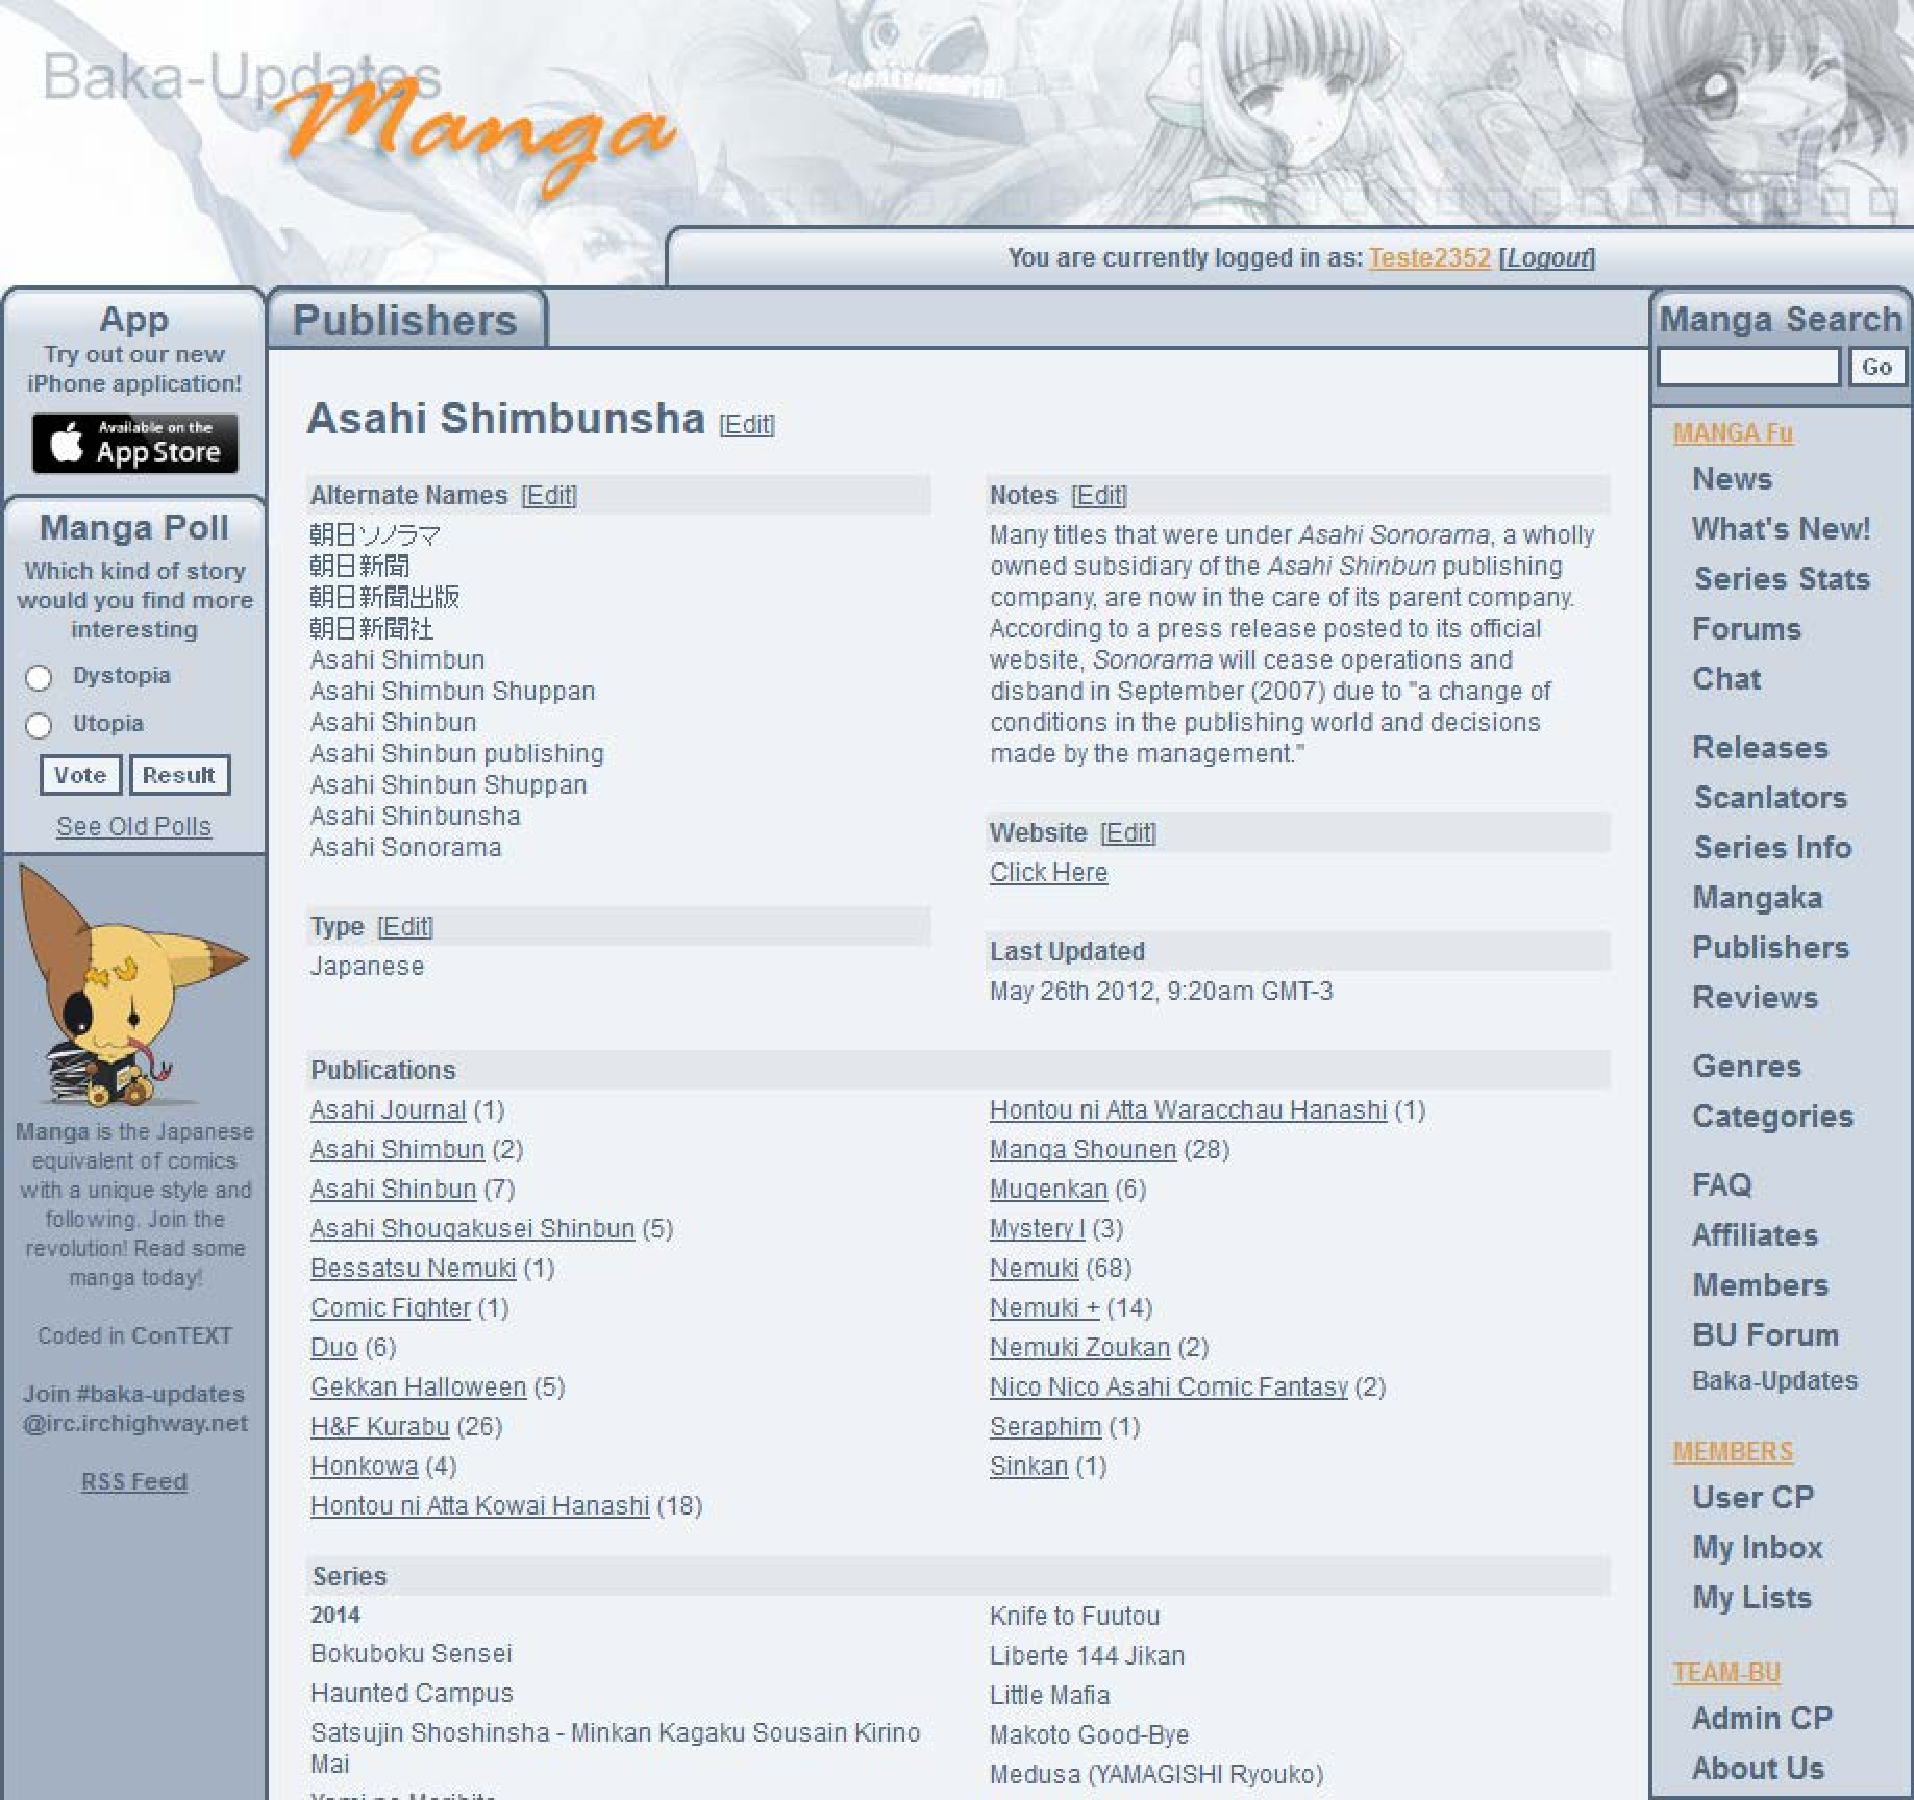
\includegraphics[height=6in,width=1\textwidth]{asahi.pdf}
\caption{Página do website Manga-Updates exibindo dados de uma editora.} \label{collection}
\end{figure}

\begin{figure}[H]
\centering
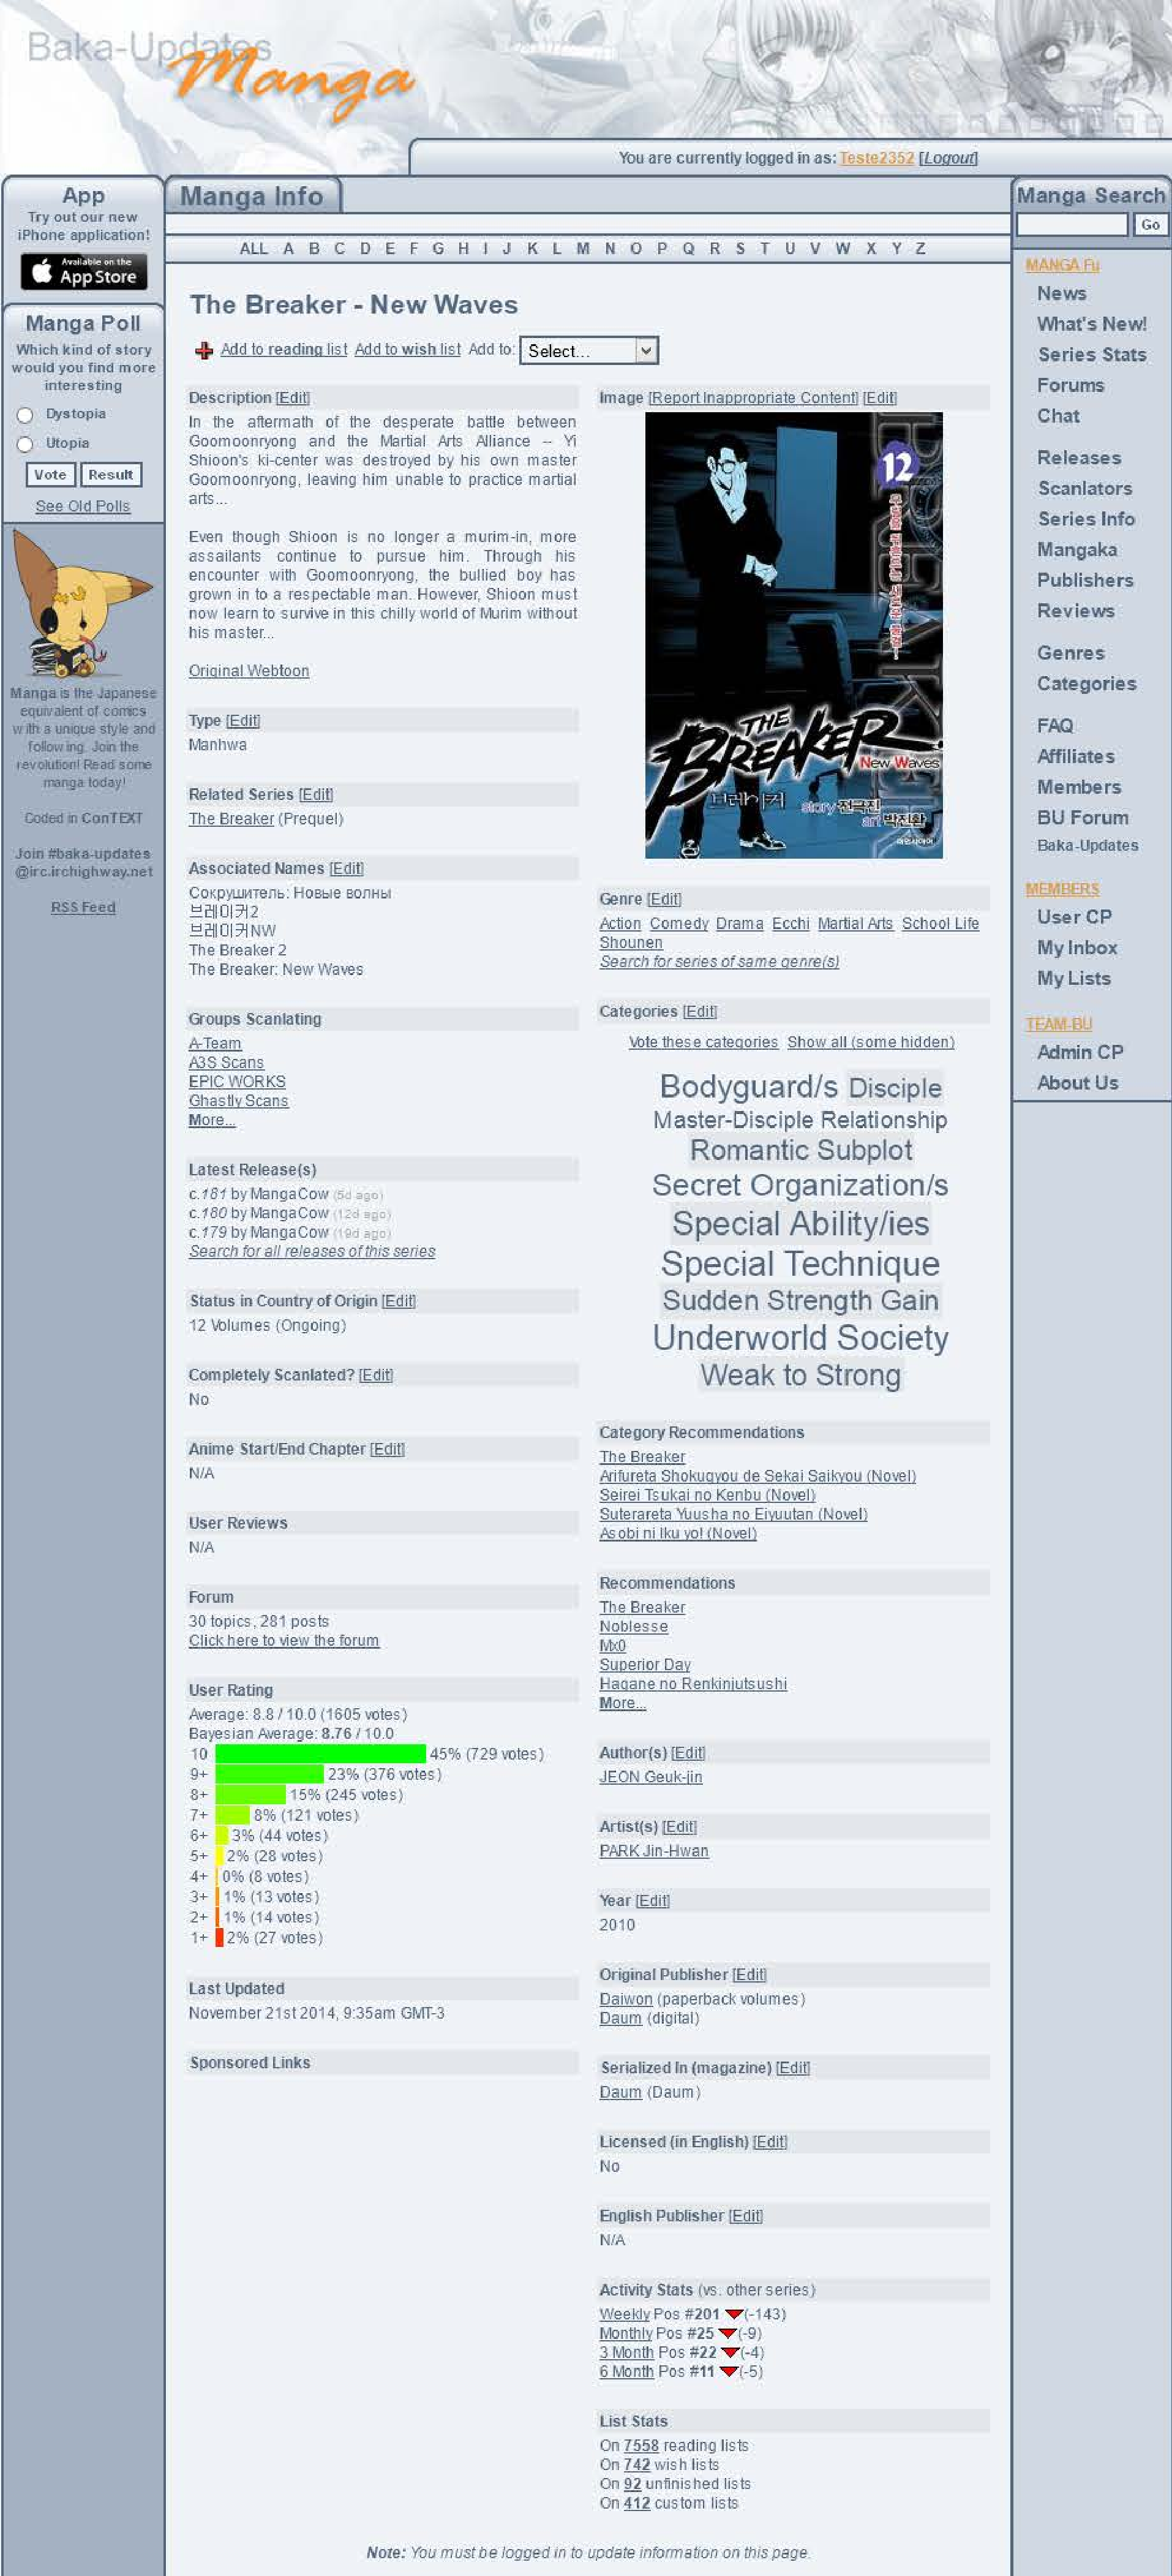
\includegraphics[height=0.95\textheight,width=0.95\textwidth]{break.pdf}
\caption{Página do website Manga-Updates exibindo dados de uma série. Neste caso uma história em quadrinhos proveniente da Coréia do Sul, referenciado como Manhwa no ocidente. Manhwa é o termo equivalente a história em quadrinhos no idioma coreano.} \label{collection}
\end{figure}

\begin{figure}[H]
\centering
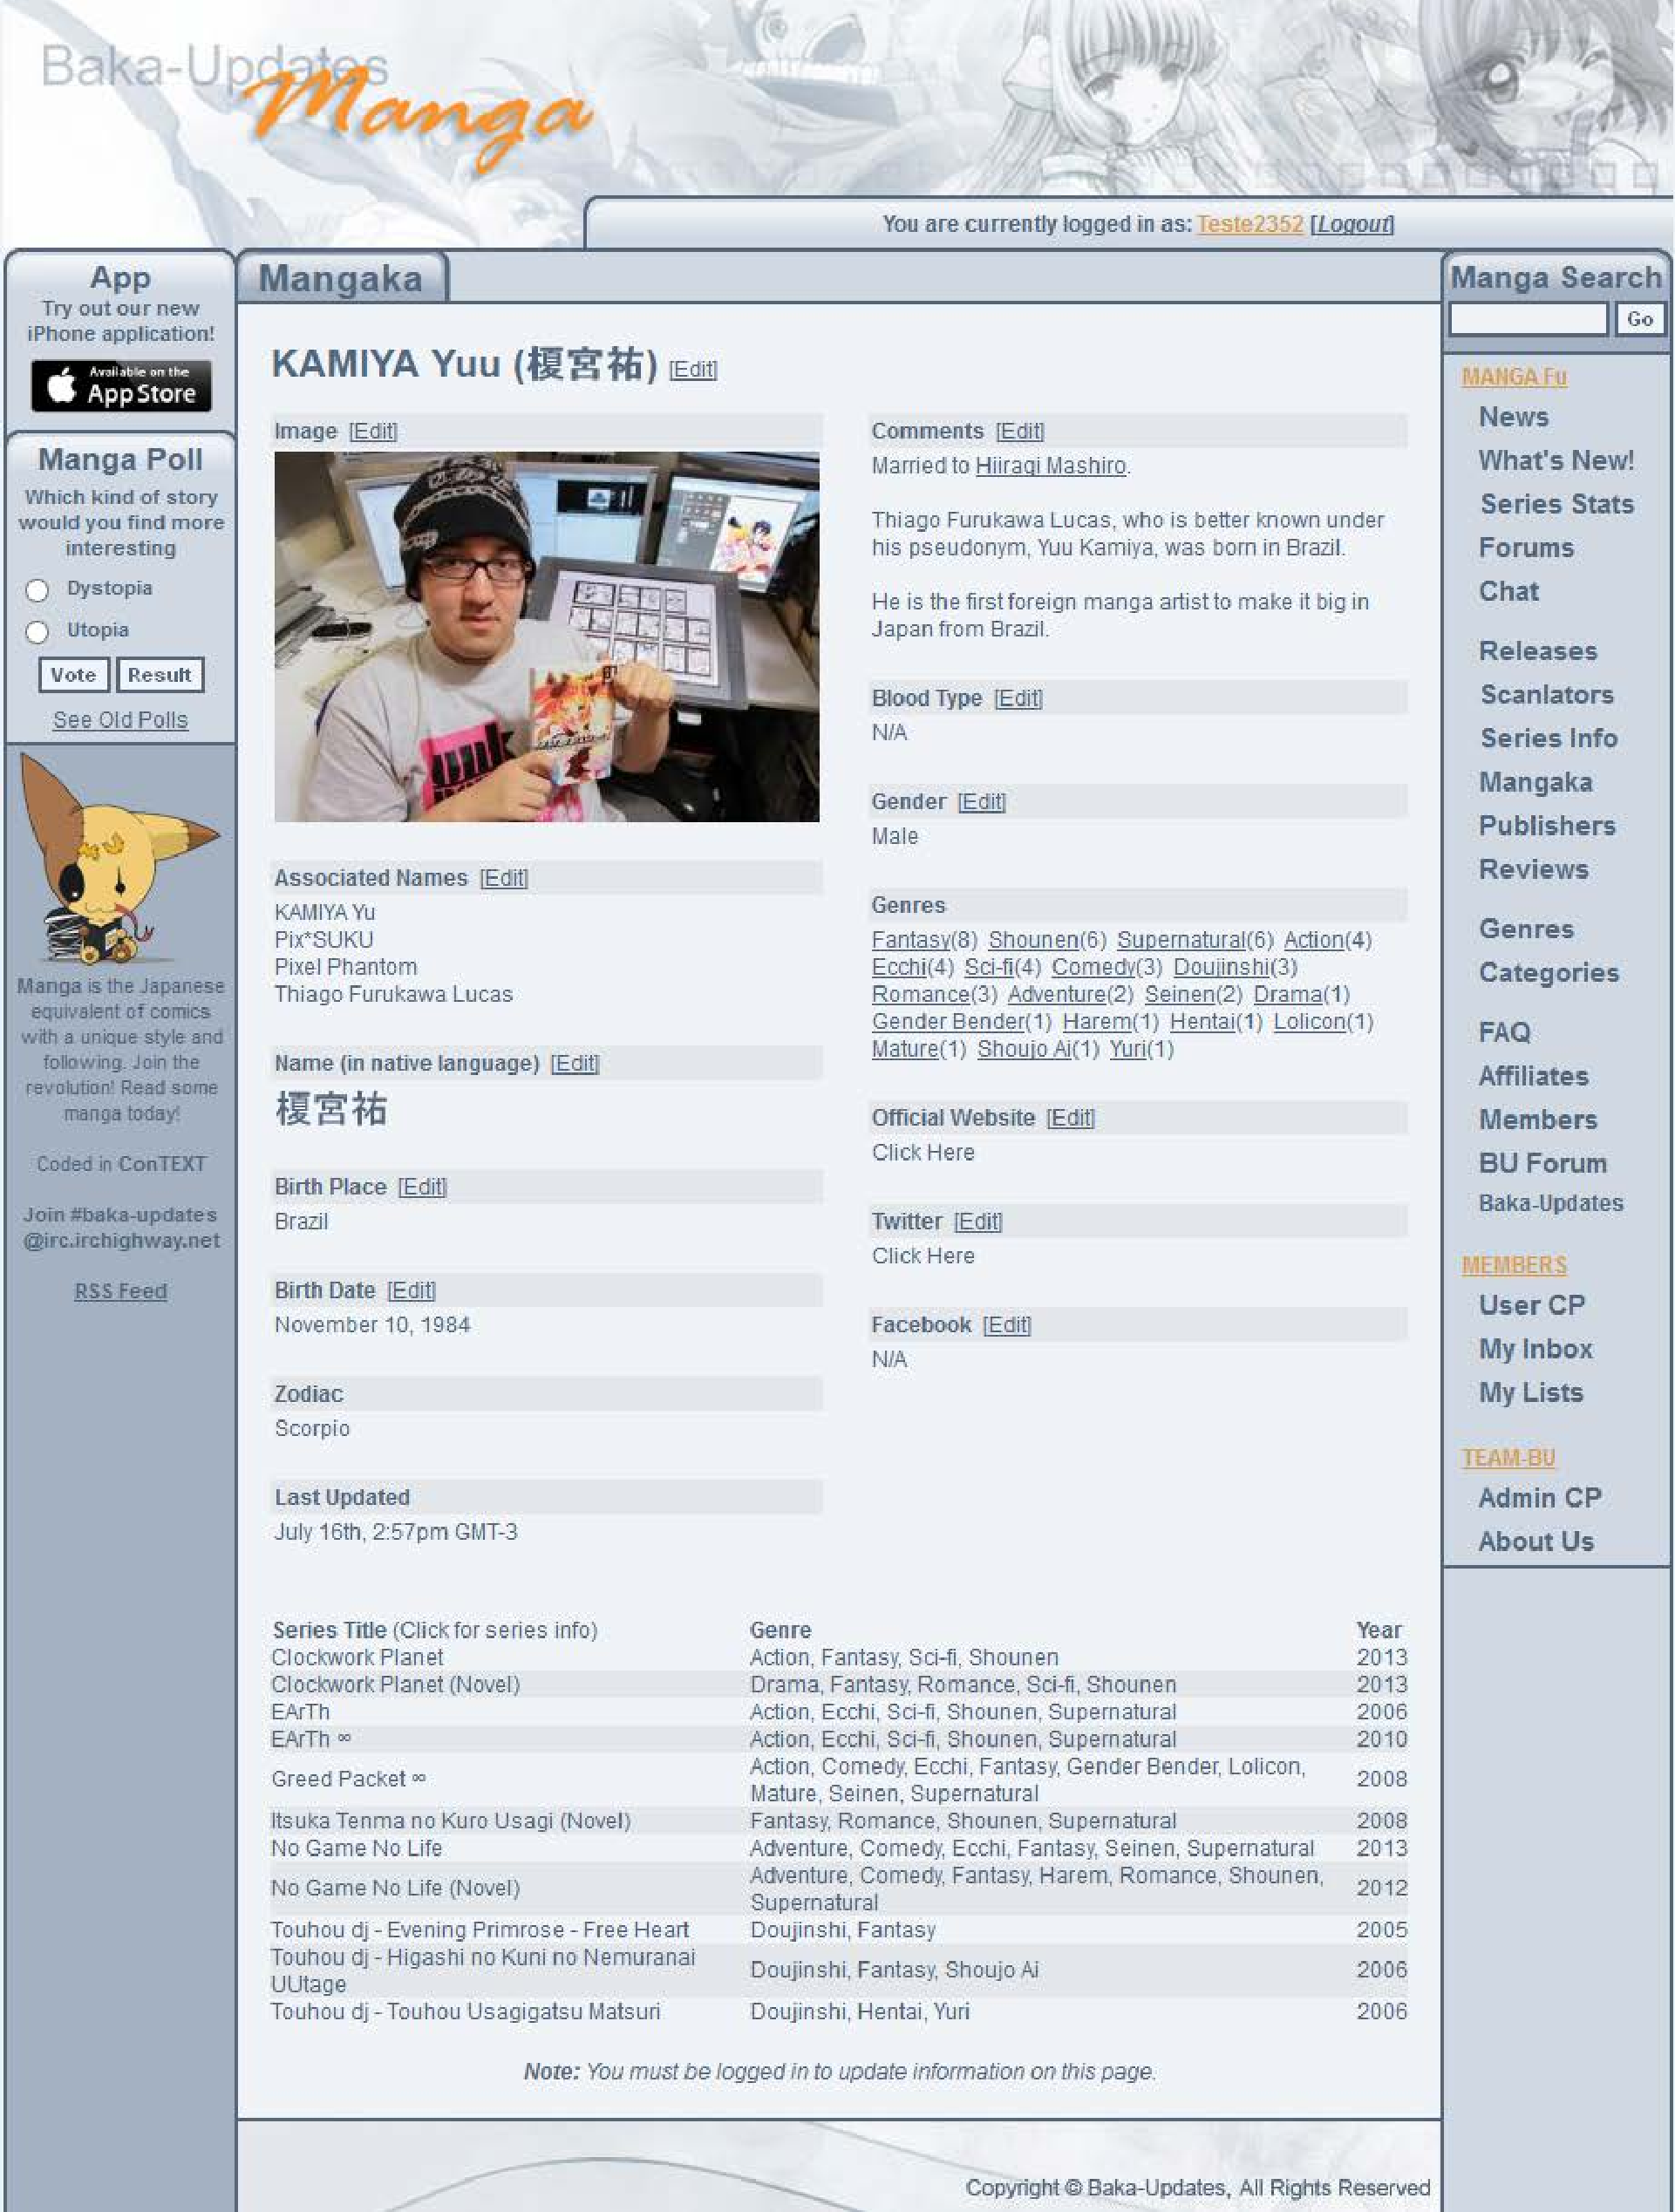
\includegraphics[width=1\textwidth]{kamiya.pdf}
\caption{Página do website Manga-Updates exibindo dados de um autor.} \label{collection}
\end{figure}


\begin{figure}[H]
\centering
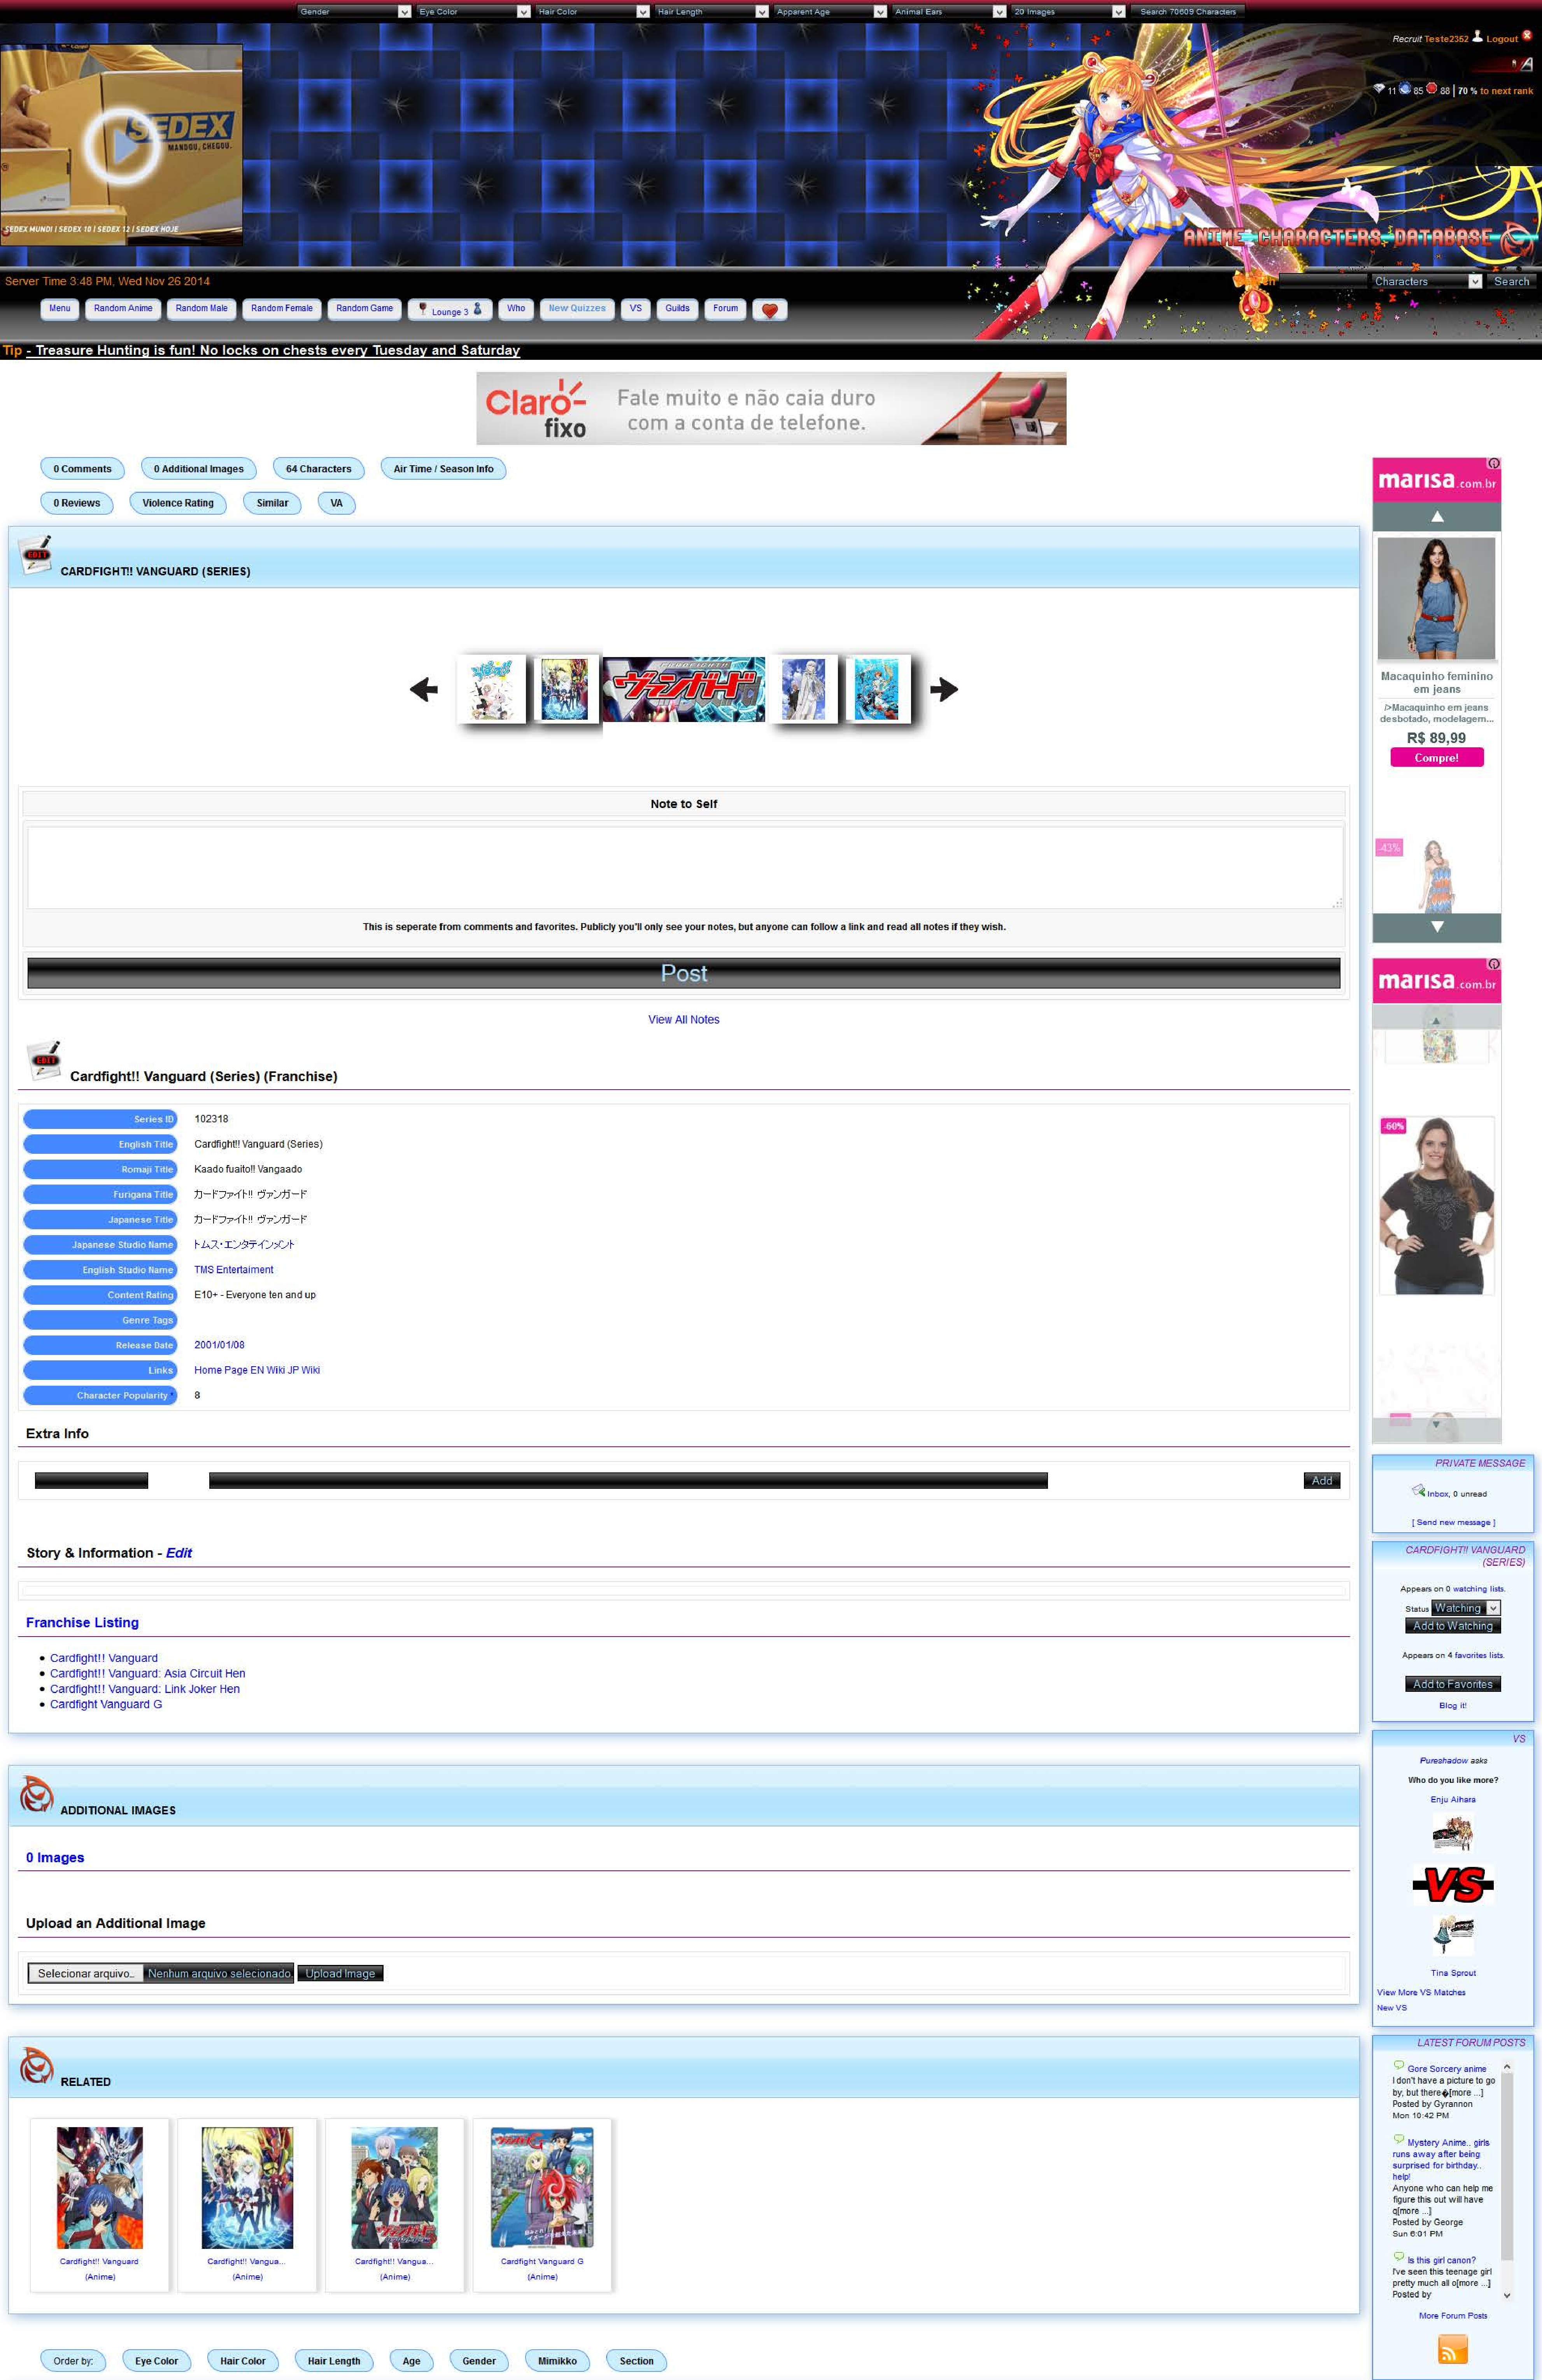
\includegraphics[width=1\textwidth]{Cardfight.pdf}
\caption{Página do website AnimeCharacterDatabase exibindo dados de um anime.} \label{collection}
\end{figure}

\begin{figure}[H]
\centering
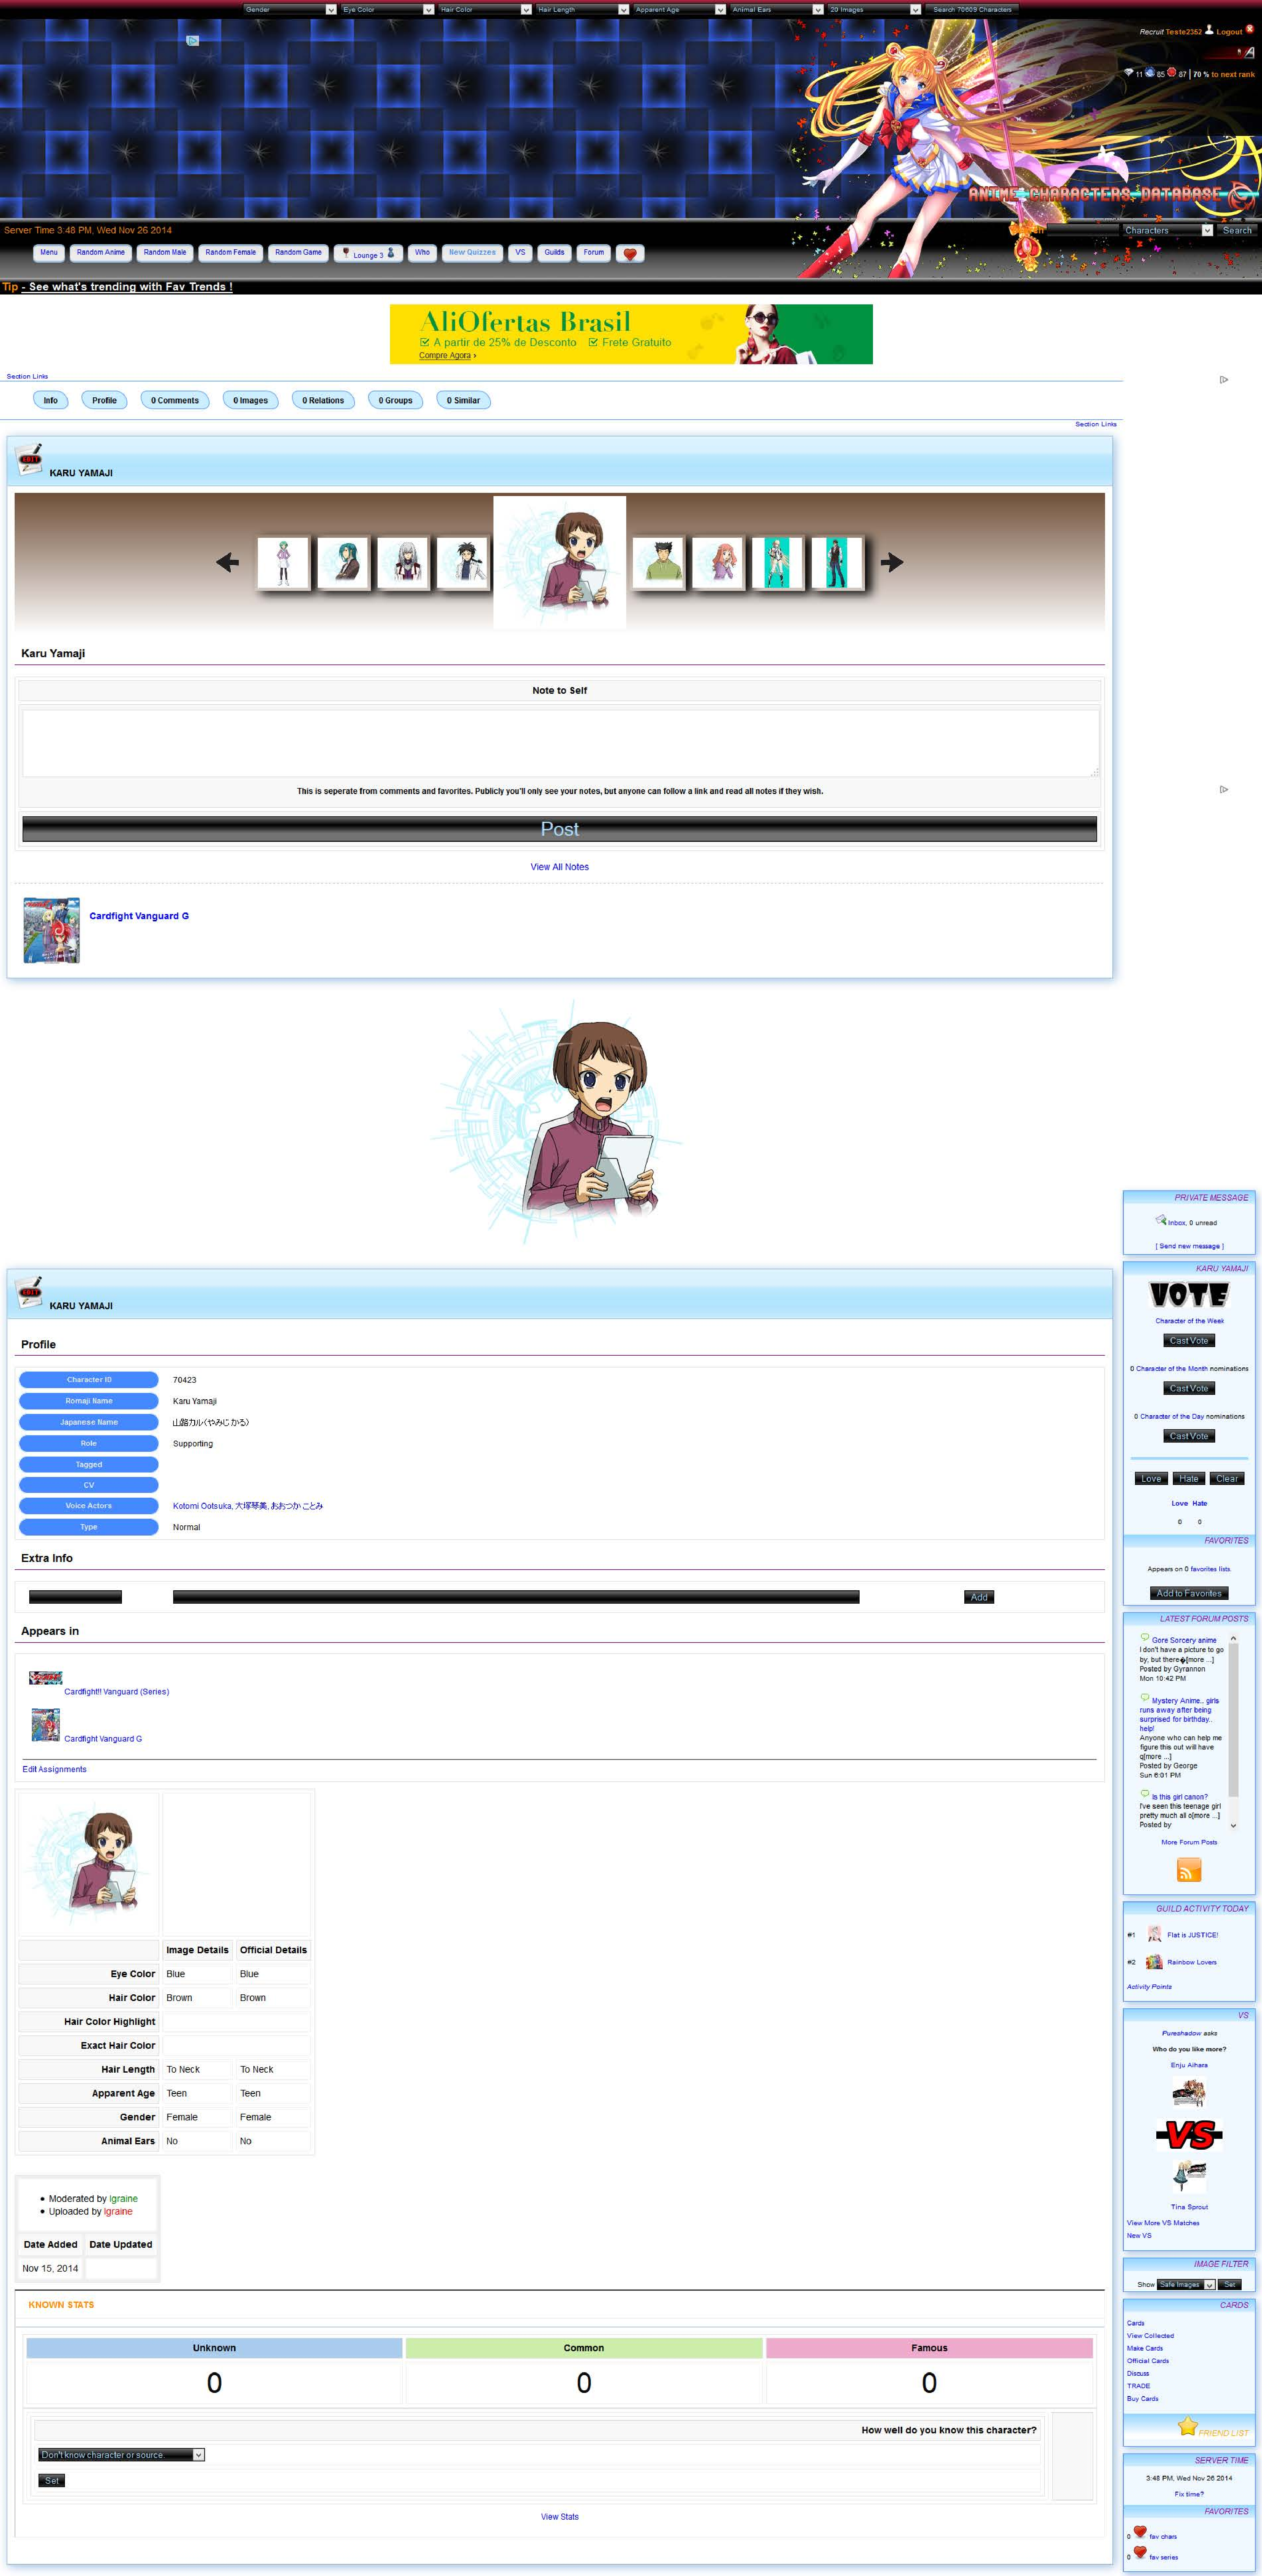
\includegraphics[height=1\textheight,width=1\textwidth]{karu.pdf}
\caption{Página do website AnimeCharacterDatabase exibindo dados de uma personagem.} \label{collection}
\end{figure}

\begin{figure}[H]
\centering
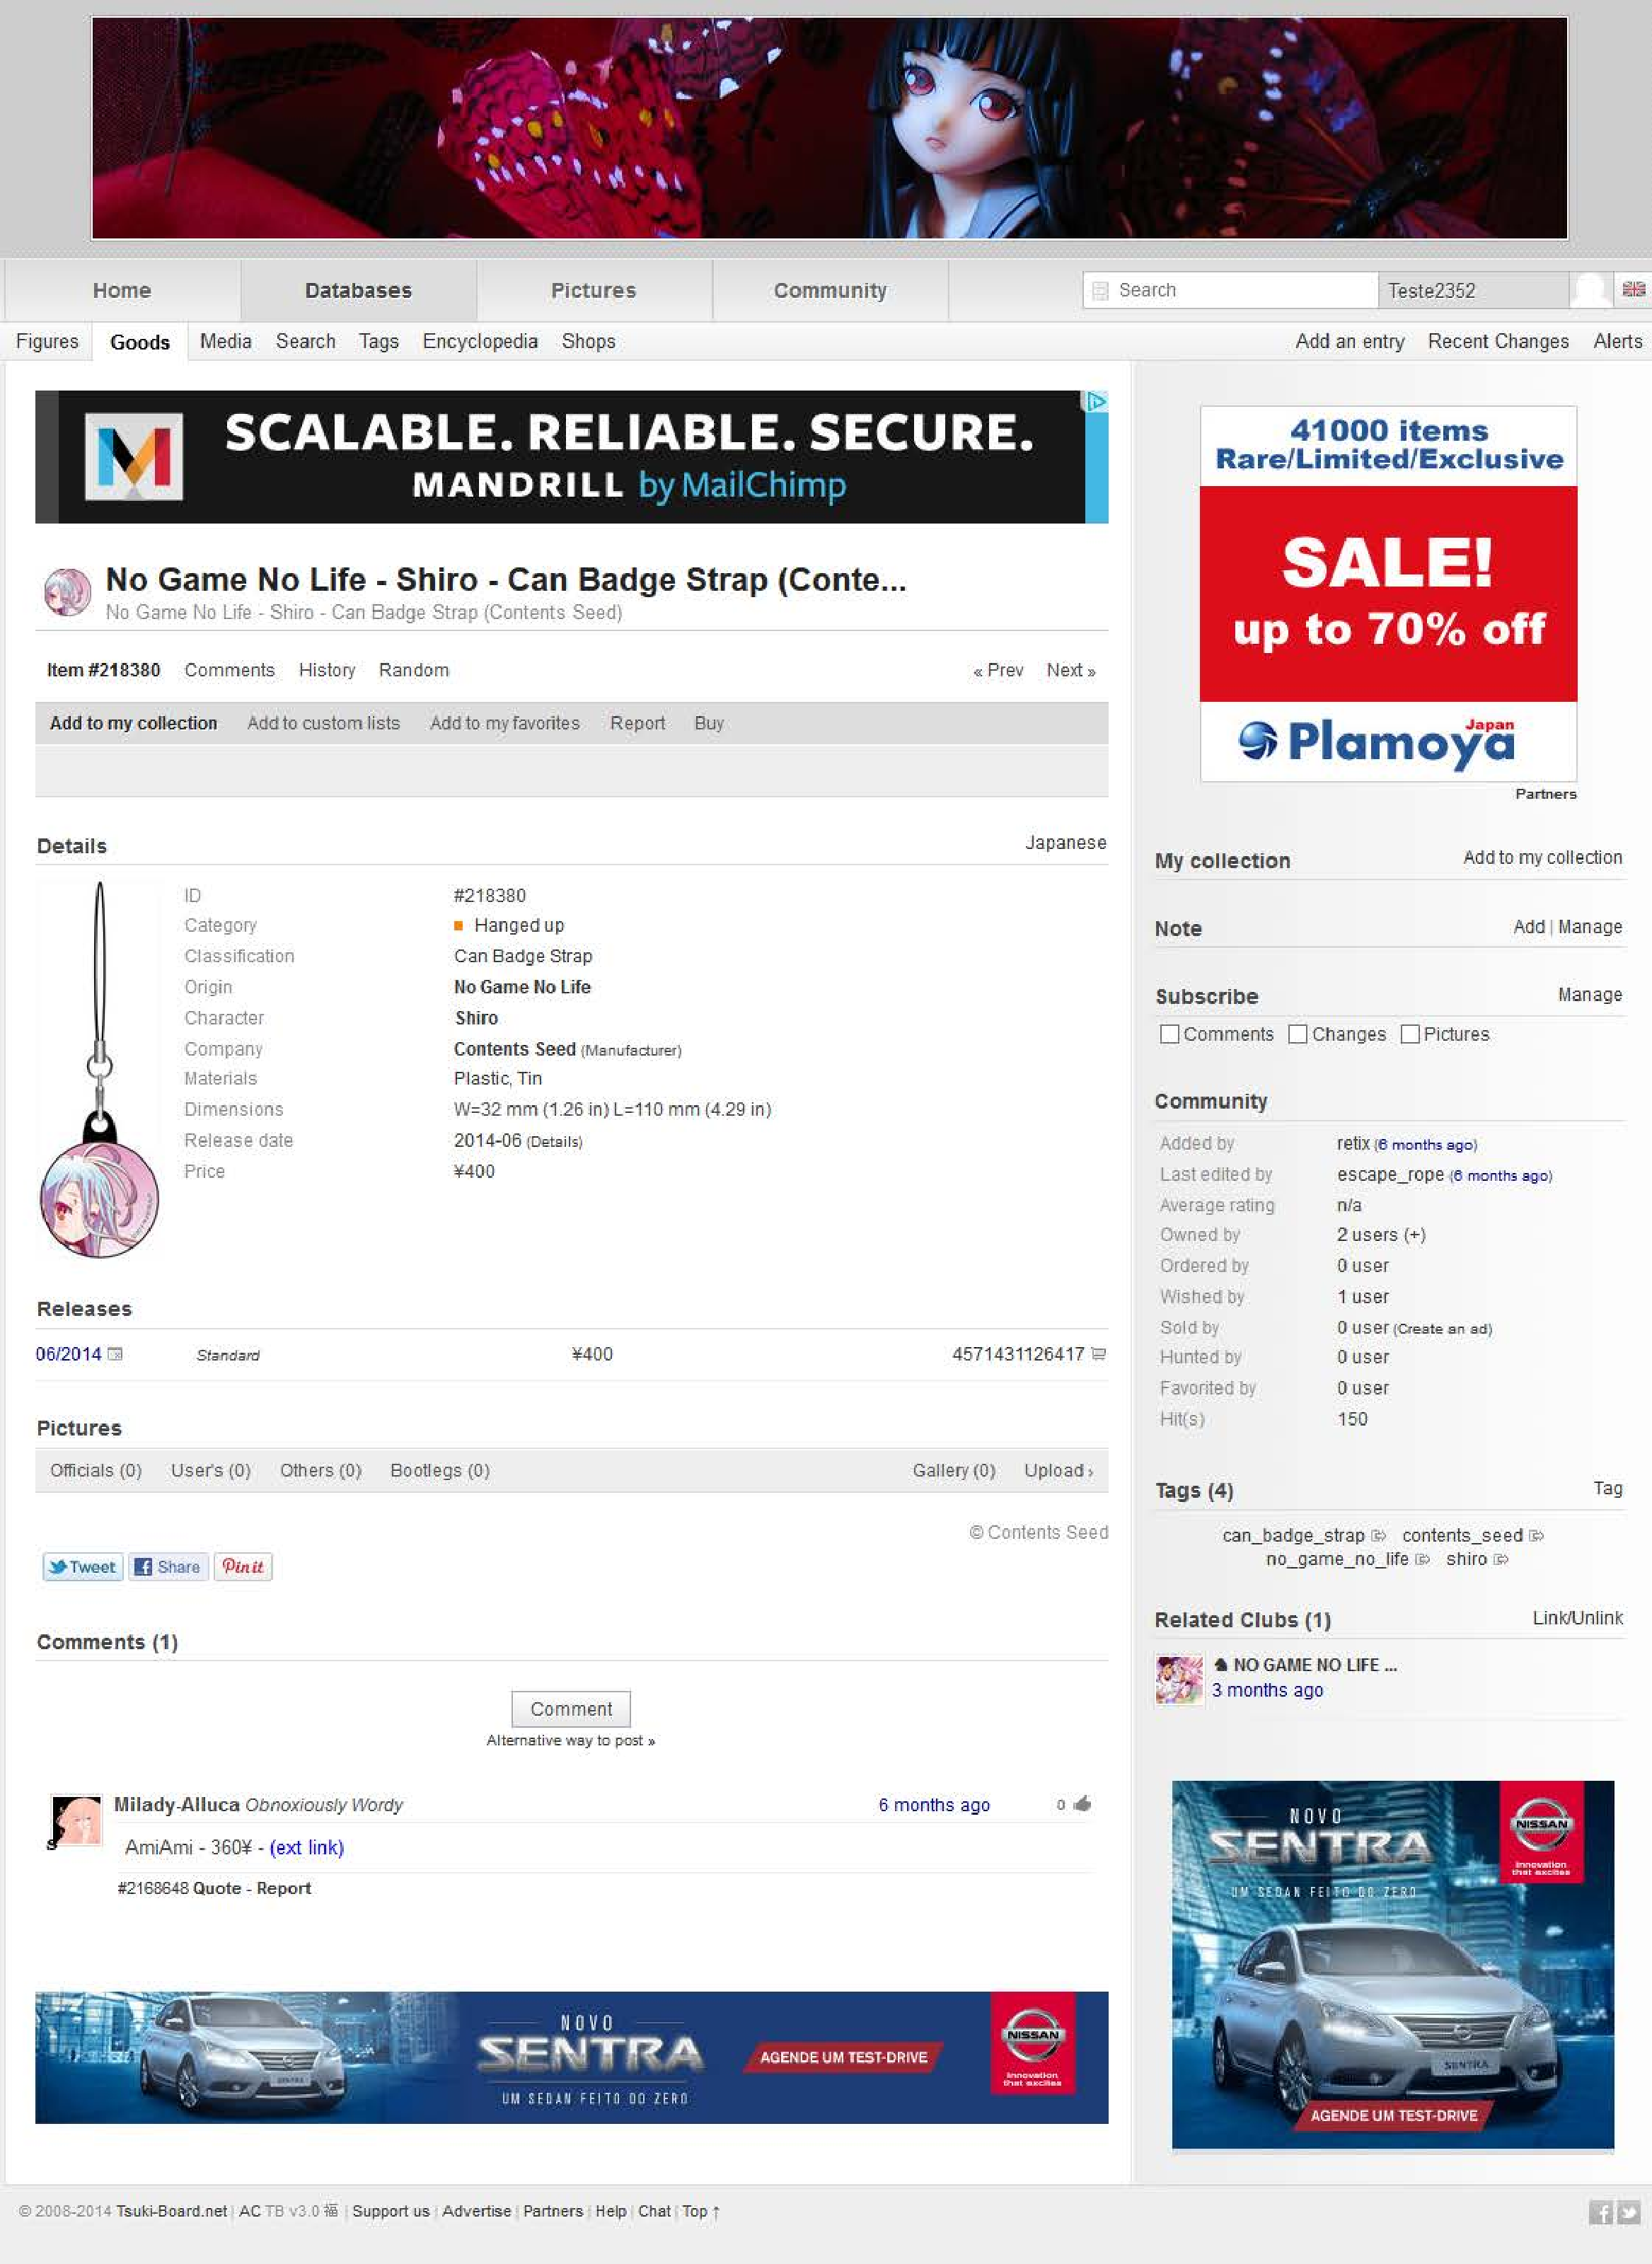
\includegraphics[width=1\textwidth]{ngnlmyfigure.pdf}
\caption{Página do website MyFigureCollection exibindo dados de um produto.} \label{collection}
\end{figure}

\begin{figure}[H]
\centering
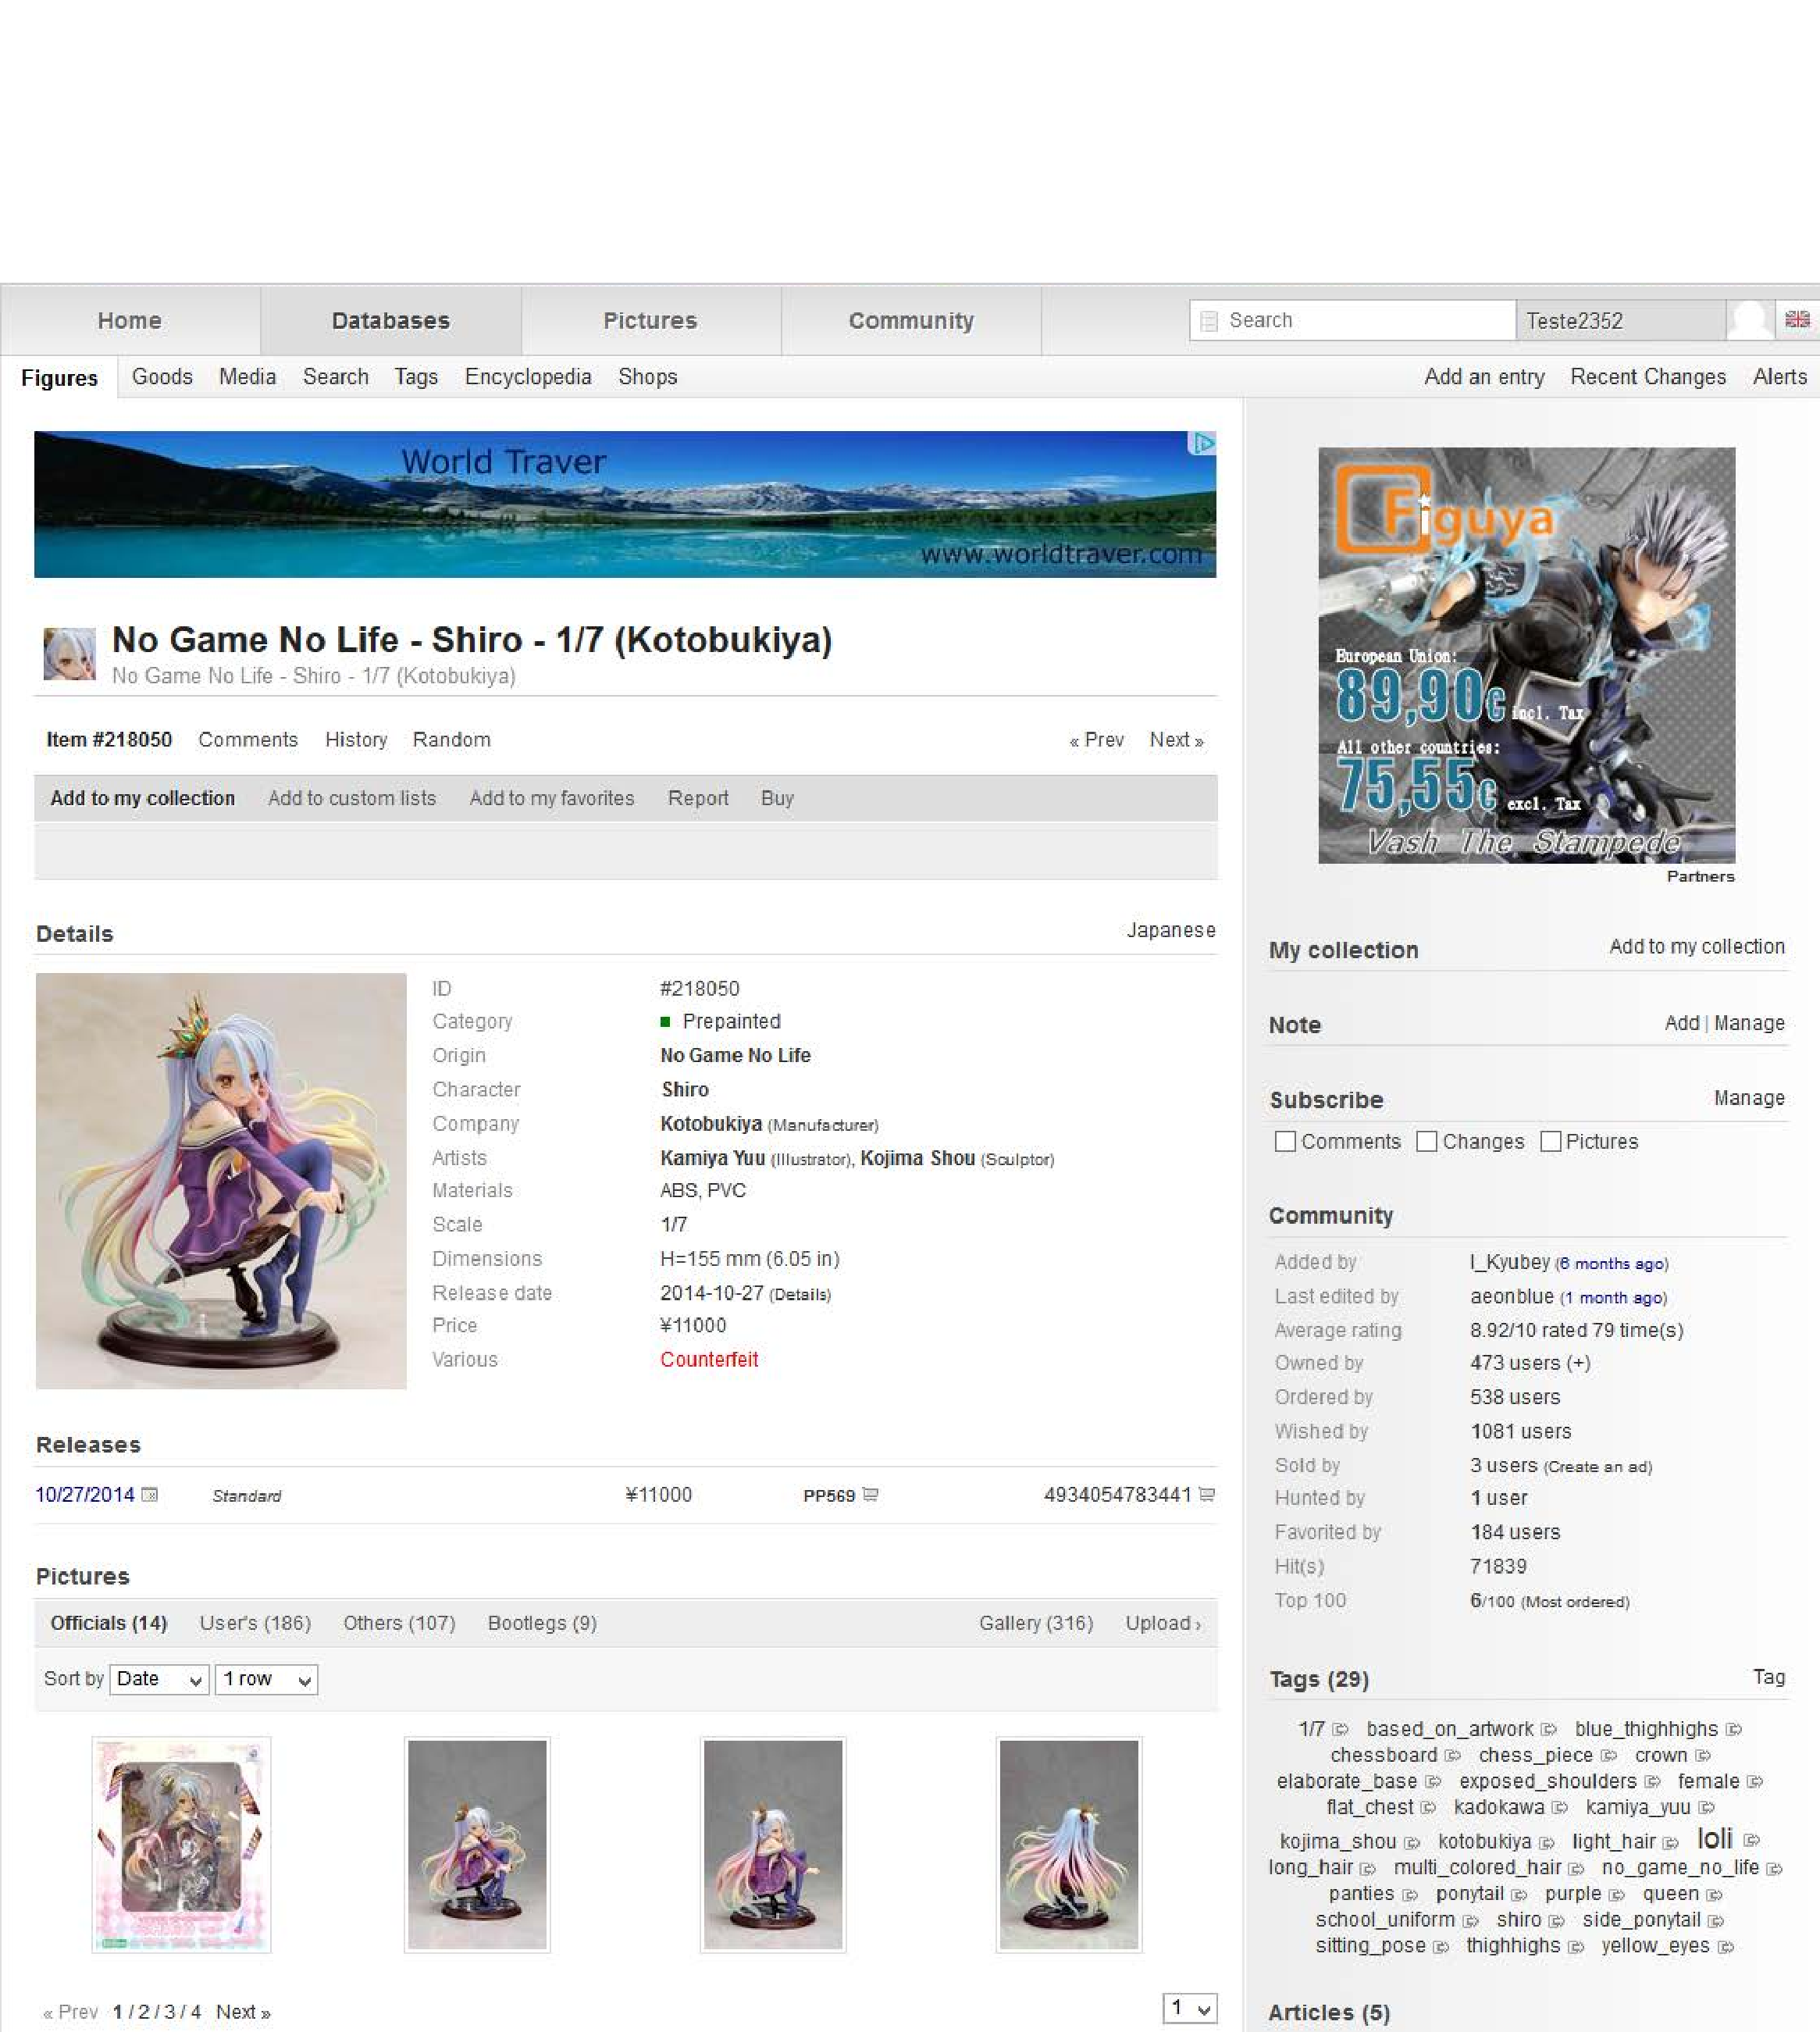
\includegraphics[height=0.45\textheight,width=0.8\textwidth]{ngnlmyfigure2.pdf}
\caption{Página do website MyFigureCollection exibindo dados de uma figura de ação.} \label{collection}
\end{figure}


%Nossa visualização de dados foca-se na ilustração quantitativa de franquias e seus produtos derivados 

\subsection{Modelagem do Banco de Dados}

Para desenvolvimento do sistema de crawling dos websites optamos por criar um Banco de Dados normalizado para que quando extraíssemos e salvassemos as informações desses websites, os dados já seriam salvos em uma estrutura normalizada. 
Portanto foram desenvolvidos o Modelo Conceitual, Modelo Relacional e Modelo Lógico do Banco de Dados. 

Para o Sistema de Banco de Dados Relacional foi escolhido o PostgreSQL, sob licença BSD, disponível para diversos sistemas operacionais, por possibilitar o uso de recursos para controle de transação, que segue o modelo ACID, e por possibilitar orientação a objeto permitindo o uso de herança entre tabelas. A orientação a objeto poderia ser utilizada para tabelas com relacionamento de generalização/especialização. 

%Este trabalho faz uso extenso de Commit e Rollback no tratamento de erros, assim transações com falhas parciais são descartadas evitando o salvamento de conteúdo incompleto.
%Como para extração dos dados dos websites escolhidos é necessário 
%Com a mentalidade que é melhor pegar todas as informações disponibilizadas pois é melhor ter que precisar e não ter, foi modelado um Banco de Dados que expandiu o conceito original e possibilita a inserção de dados relacionais para armazenamento de músicas, vídeos, livros e diversas informações associadas. 

\subsubsection{Modelo Conceitual}

Com o estudo do conteúdo dos websites escolhidos, o conceito inicial de armazenar dados sobre mangás, animes e Light Novels resultou em um Modelo Conceitual expandido que possibilita a inserção de diversos dados relacionadas a franquias como músicas, softwares, vídeos e livros, além de permitir o cadastro de qualquer pessoa e empresa envolvida na produção de algum produto.

Com a expansão do tipo de informação a ser salva no banco de dados, a criação do modelo conceitual se tornou complexa: além do tradicional uso de atributos e relacionamentos foram utilizados conceito de especialização/generalização e associação. 

Como a estrutura do Modelo Conceitual é complexa dividimos sua ilustração em partes. Para melhor compreensão, antes de apresentarmos cada parte mostraremos um diagrama mais simples abrangendo as principais entidades do Modelo Conceitual:

\begin{figure}[H]
\centering
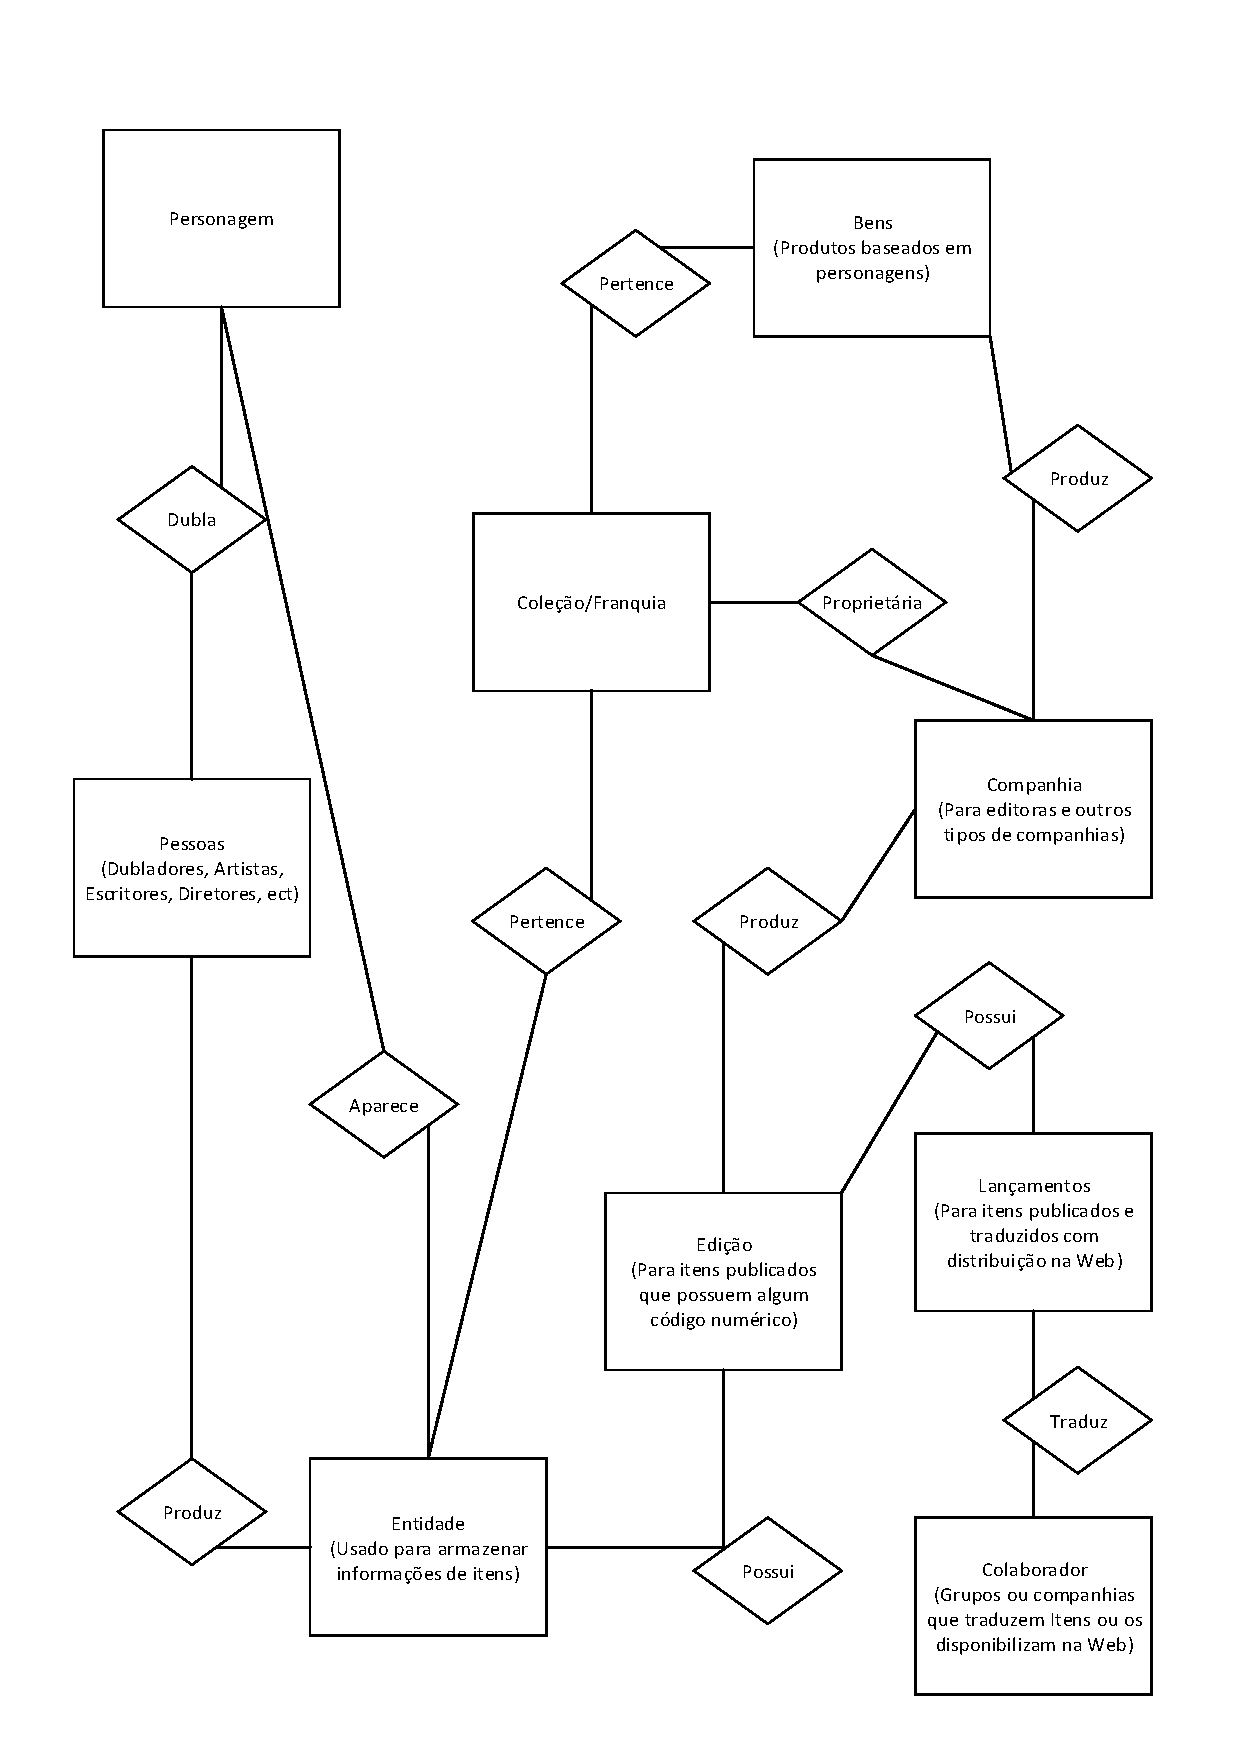
\includegraphics[height=0.8\textheight,width=0.9\textwidth]{MER_-_General.pdf}
\caption{Modelo Conceitual resumido com os nomes das principais entidades em português. No Modelo Conceitual detalhado e na implementação do Modelo Lógico foram utilizados textos em inglês.} \label{collection}
\end{figure}

A seguir podem ser observados as entidades e seus relacionamentos de forma mais detalhada. As entidades na cor laranja representam entidades que serão detalhadas mais a frente.
\begin{figure}[H]
\centering
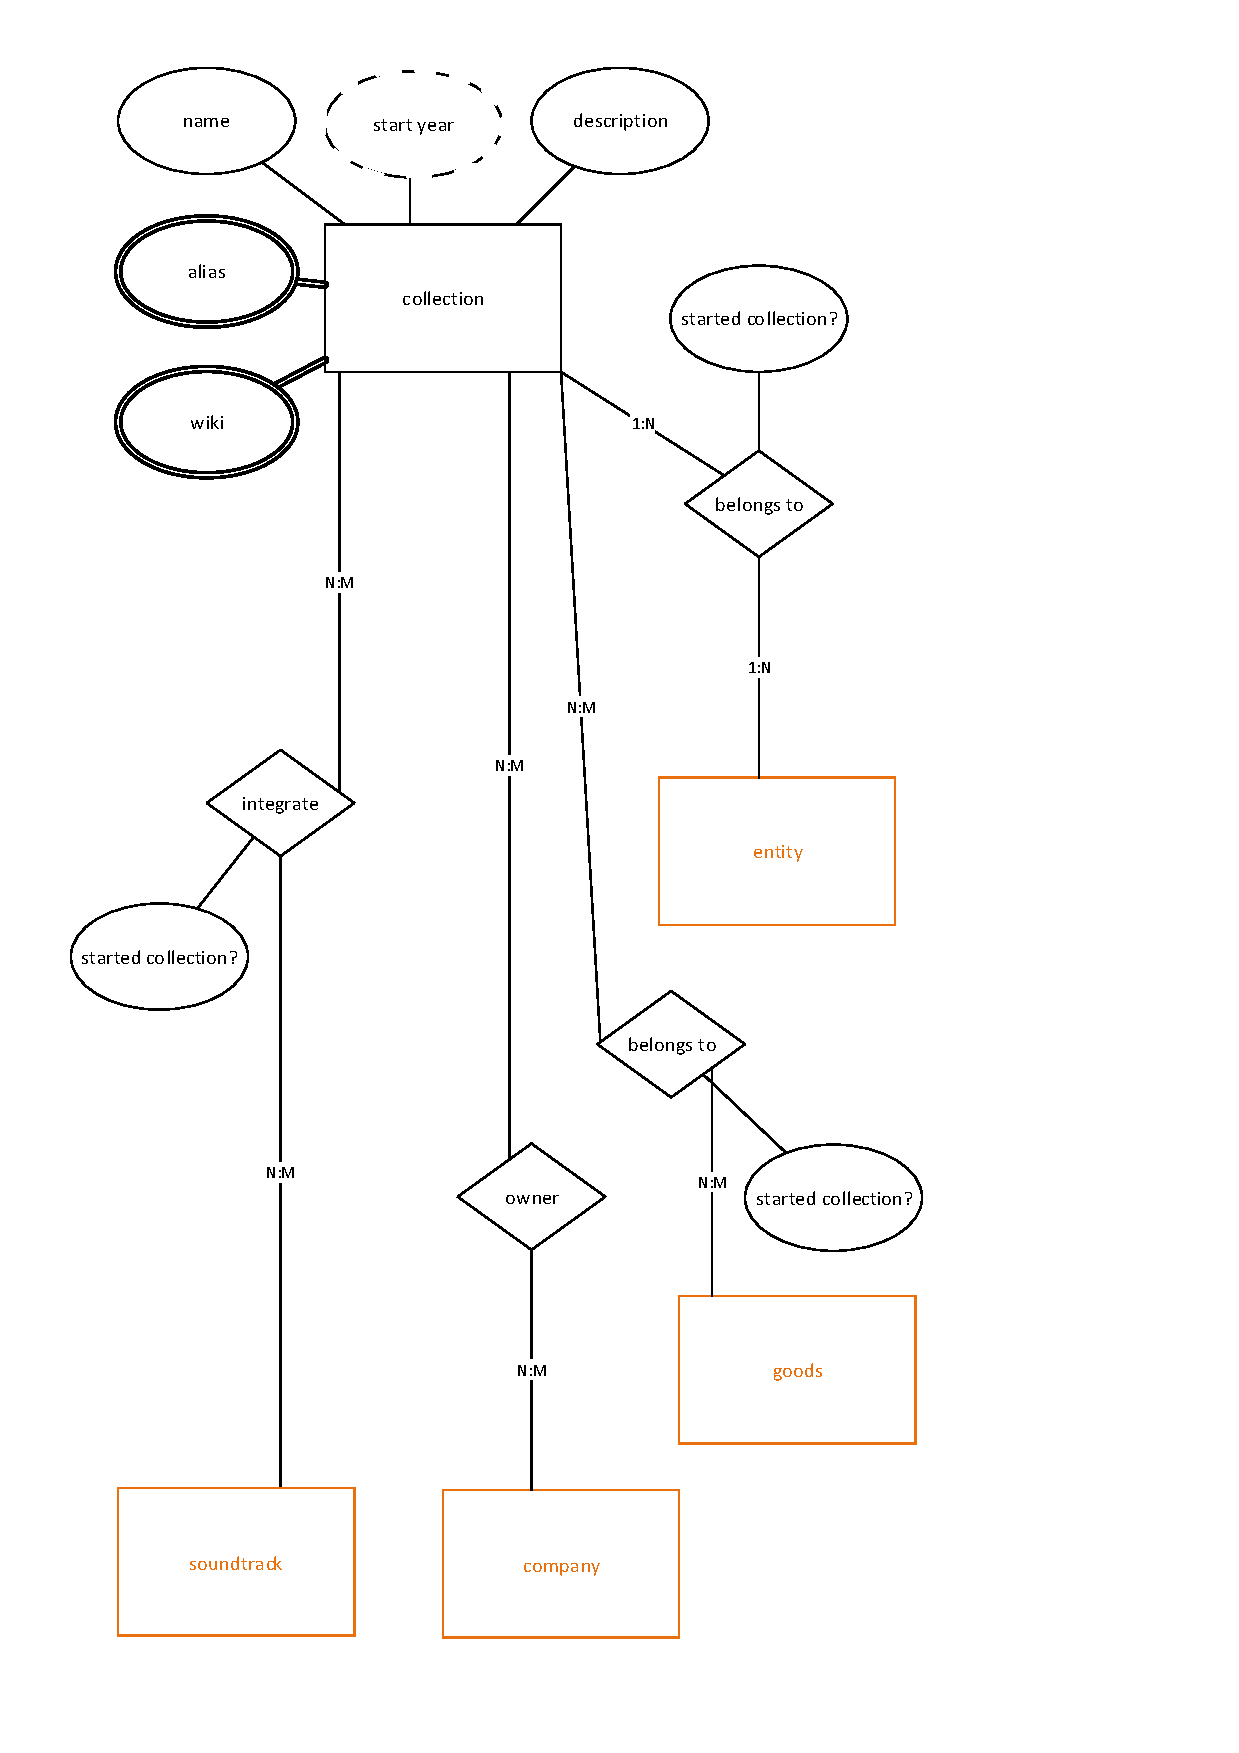
\includegraphics[height=0.85\textheight, width=0.75\textwidth]{MER_-_Collection.pdf}
\caption{\textit{Collection} é a entidade responsável por armazenar informações de franquias.} \label{collection}
\end{figure}

\begin{figure}[H]
\centering
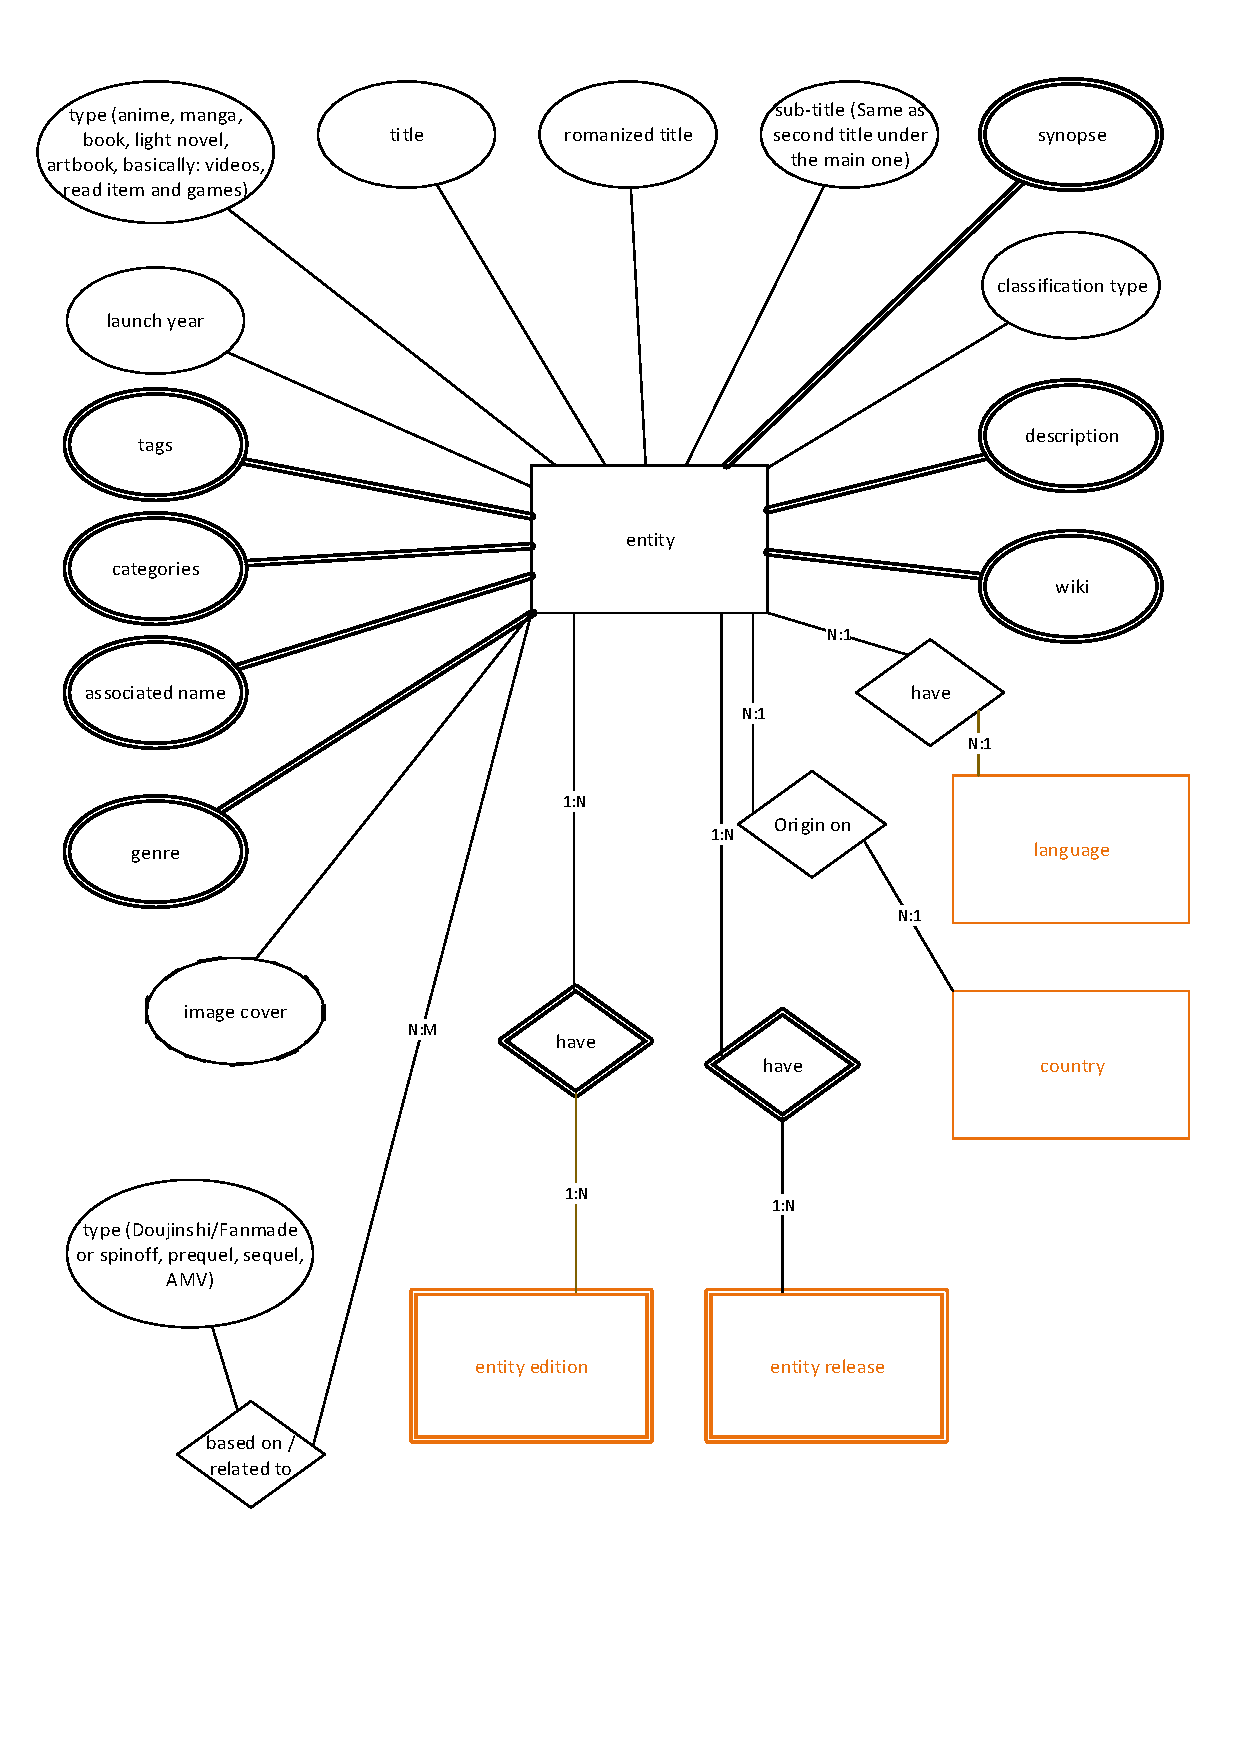
\includegraphics[width=1\textwidth]{MER_-_Entity.pdf}
\caption{\textit{Entity} é a entidade responsável por armazenar diversos tipos de conteúdo como vídeos, livros e jogos.} \label{entity}
\end{figure}

\begin{figure}[H]
\centering
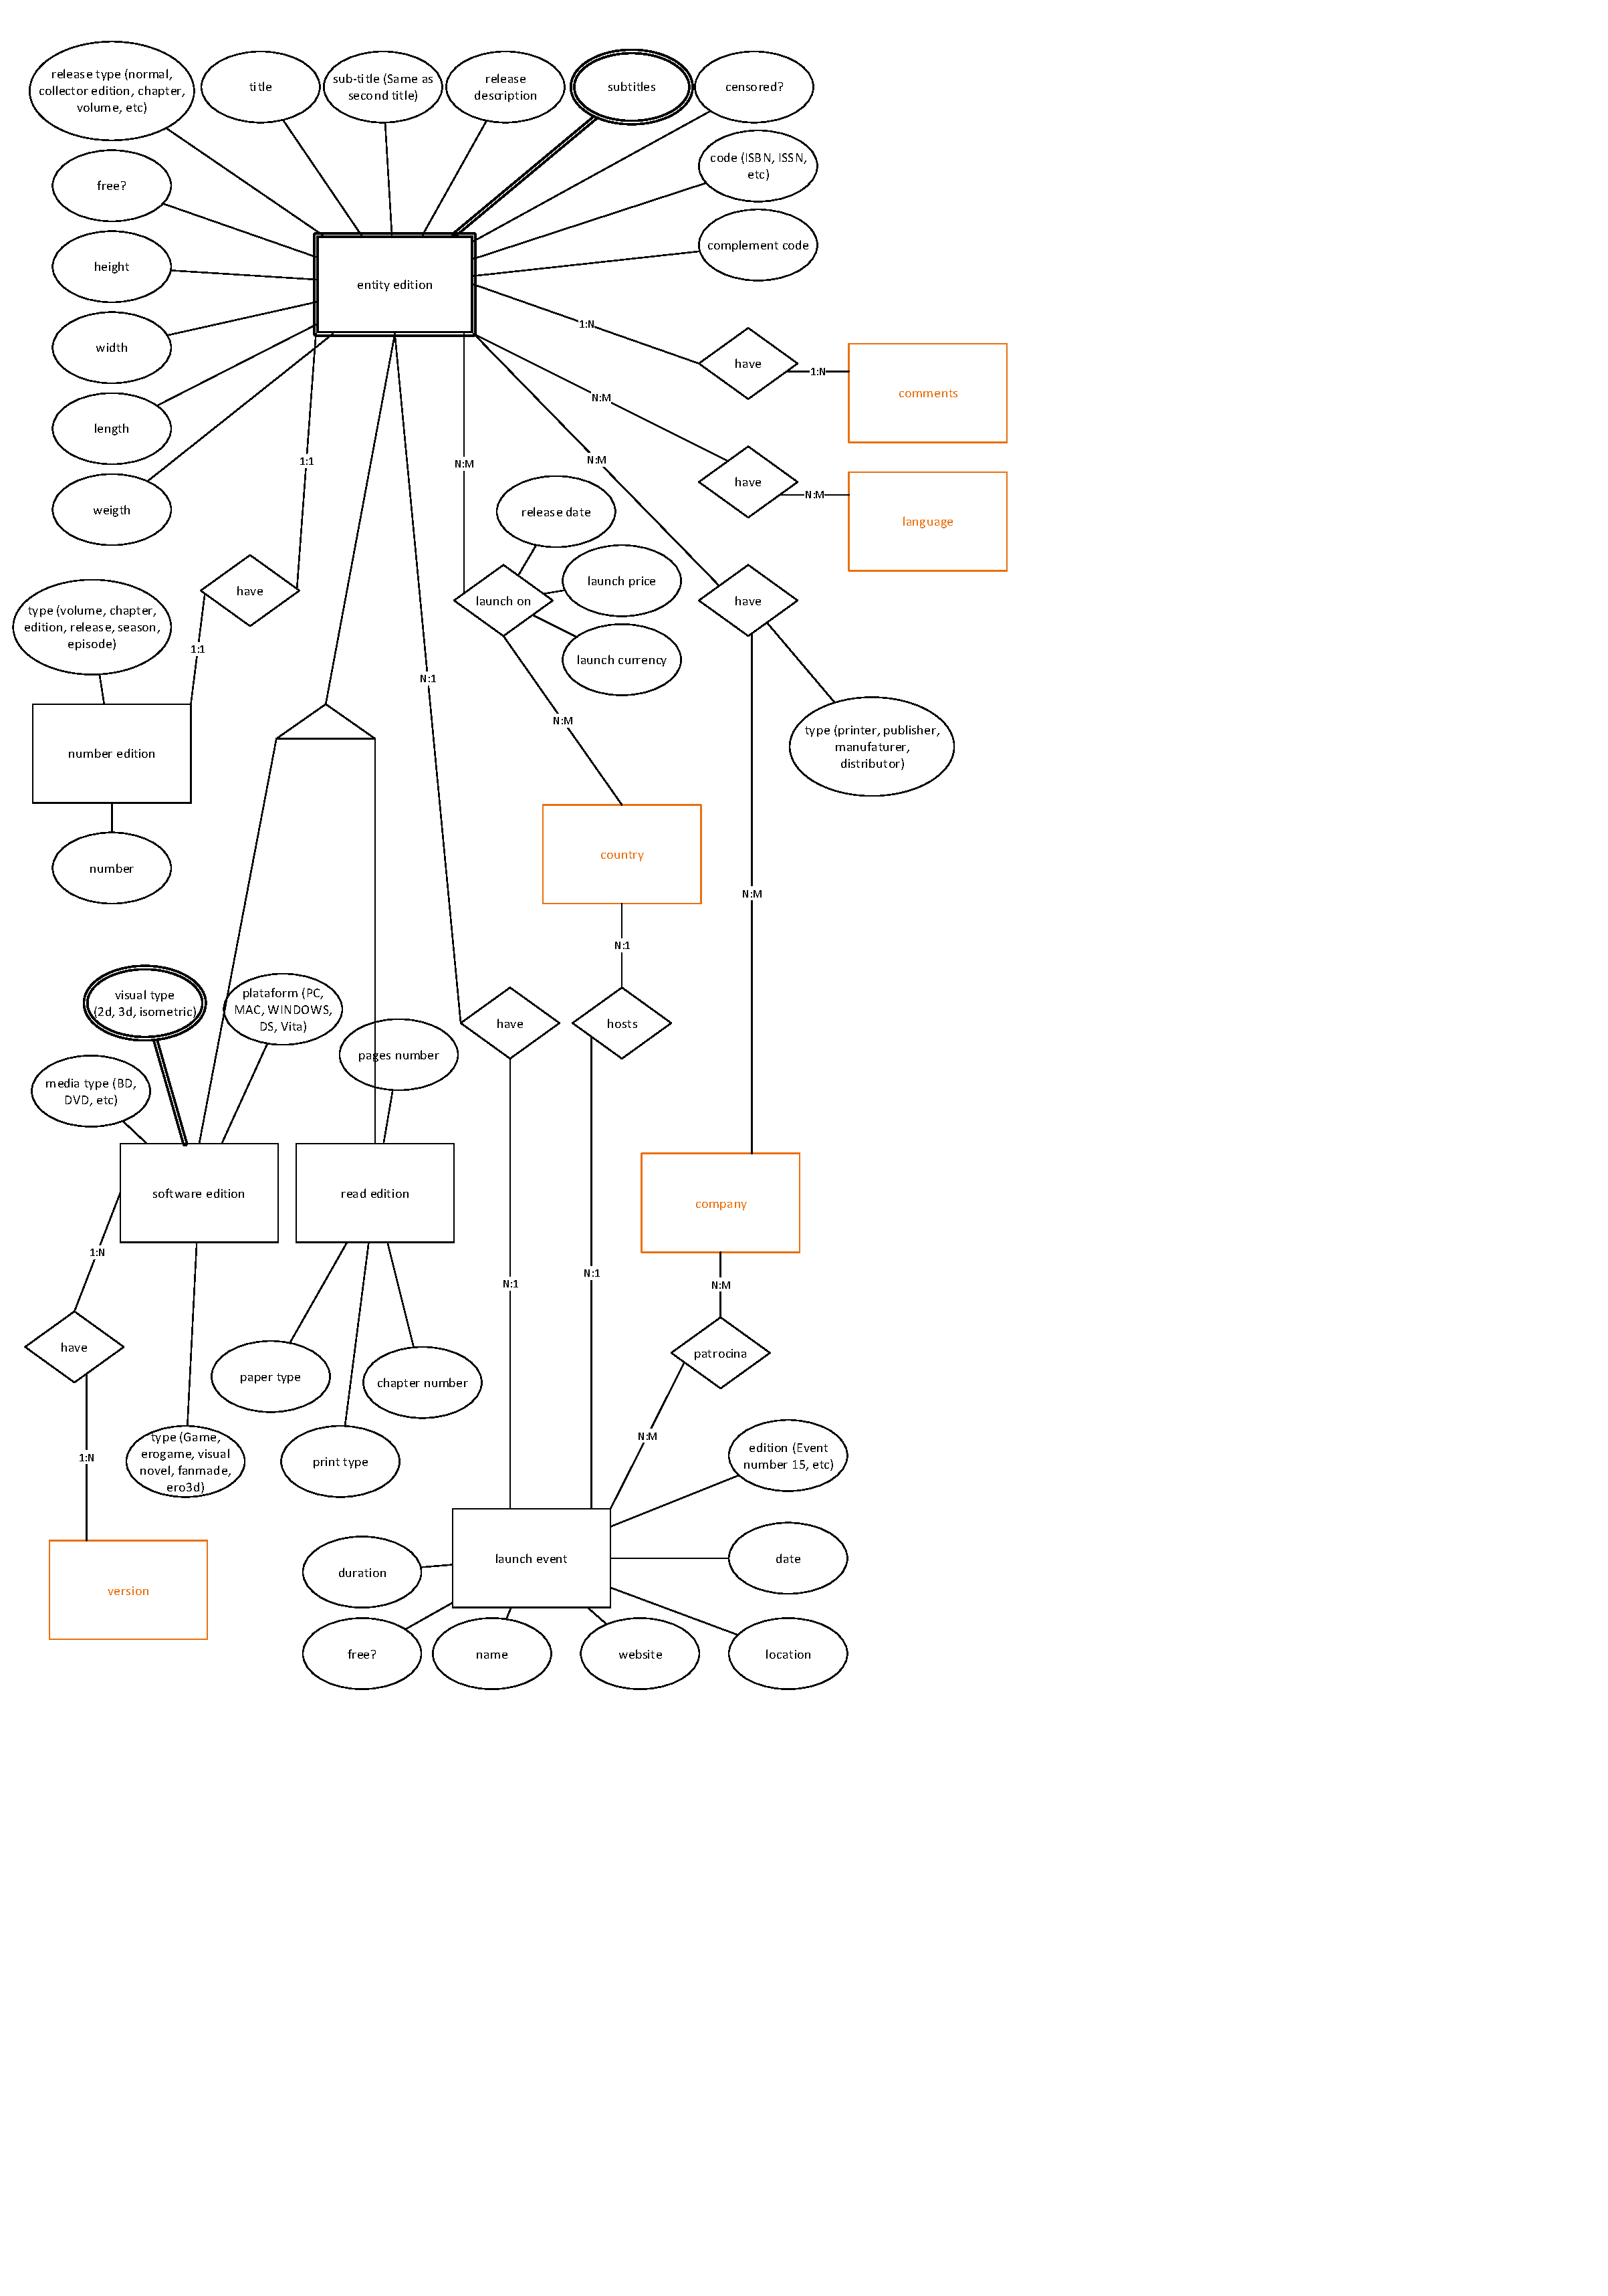
\includegraphics[height=0.9\textheight,width=0.9\textwidth]{MER_-_Edition.pdf}
\caption{\textit{Edition} é a entidade responsável por armazenar informações de itens armazenados em \textit{Entity} que possuem publicação física. A entidade \textit{Edition} se especializa em \textit{Software Edition} para armazenamento de informações especificas a softwares e \textit{Read Edition} para armazenamento de informações de livros e revistas}\label{edition}
\end{figure}

\begin{figure}[H]
\centering
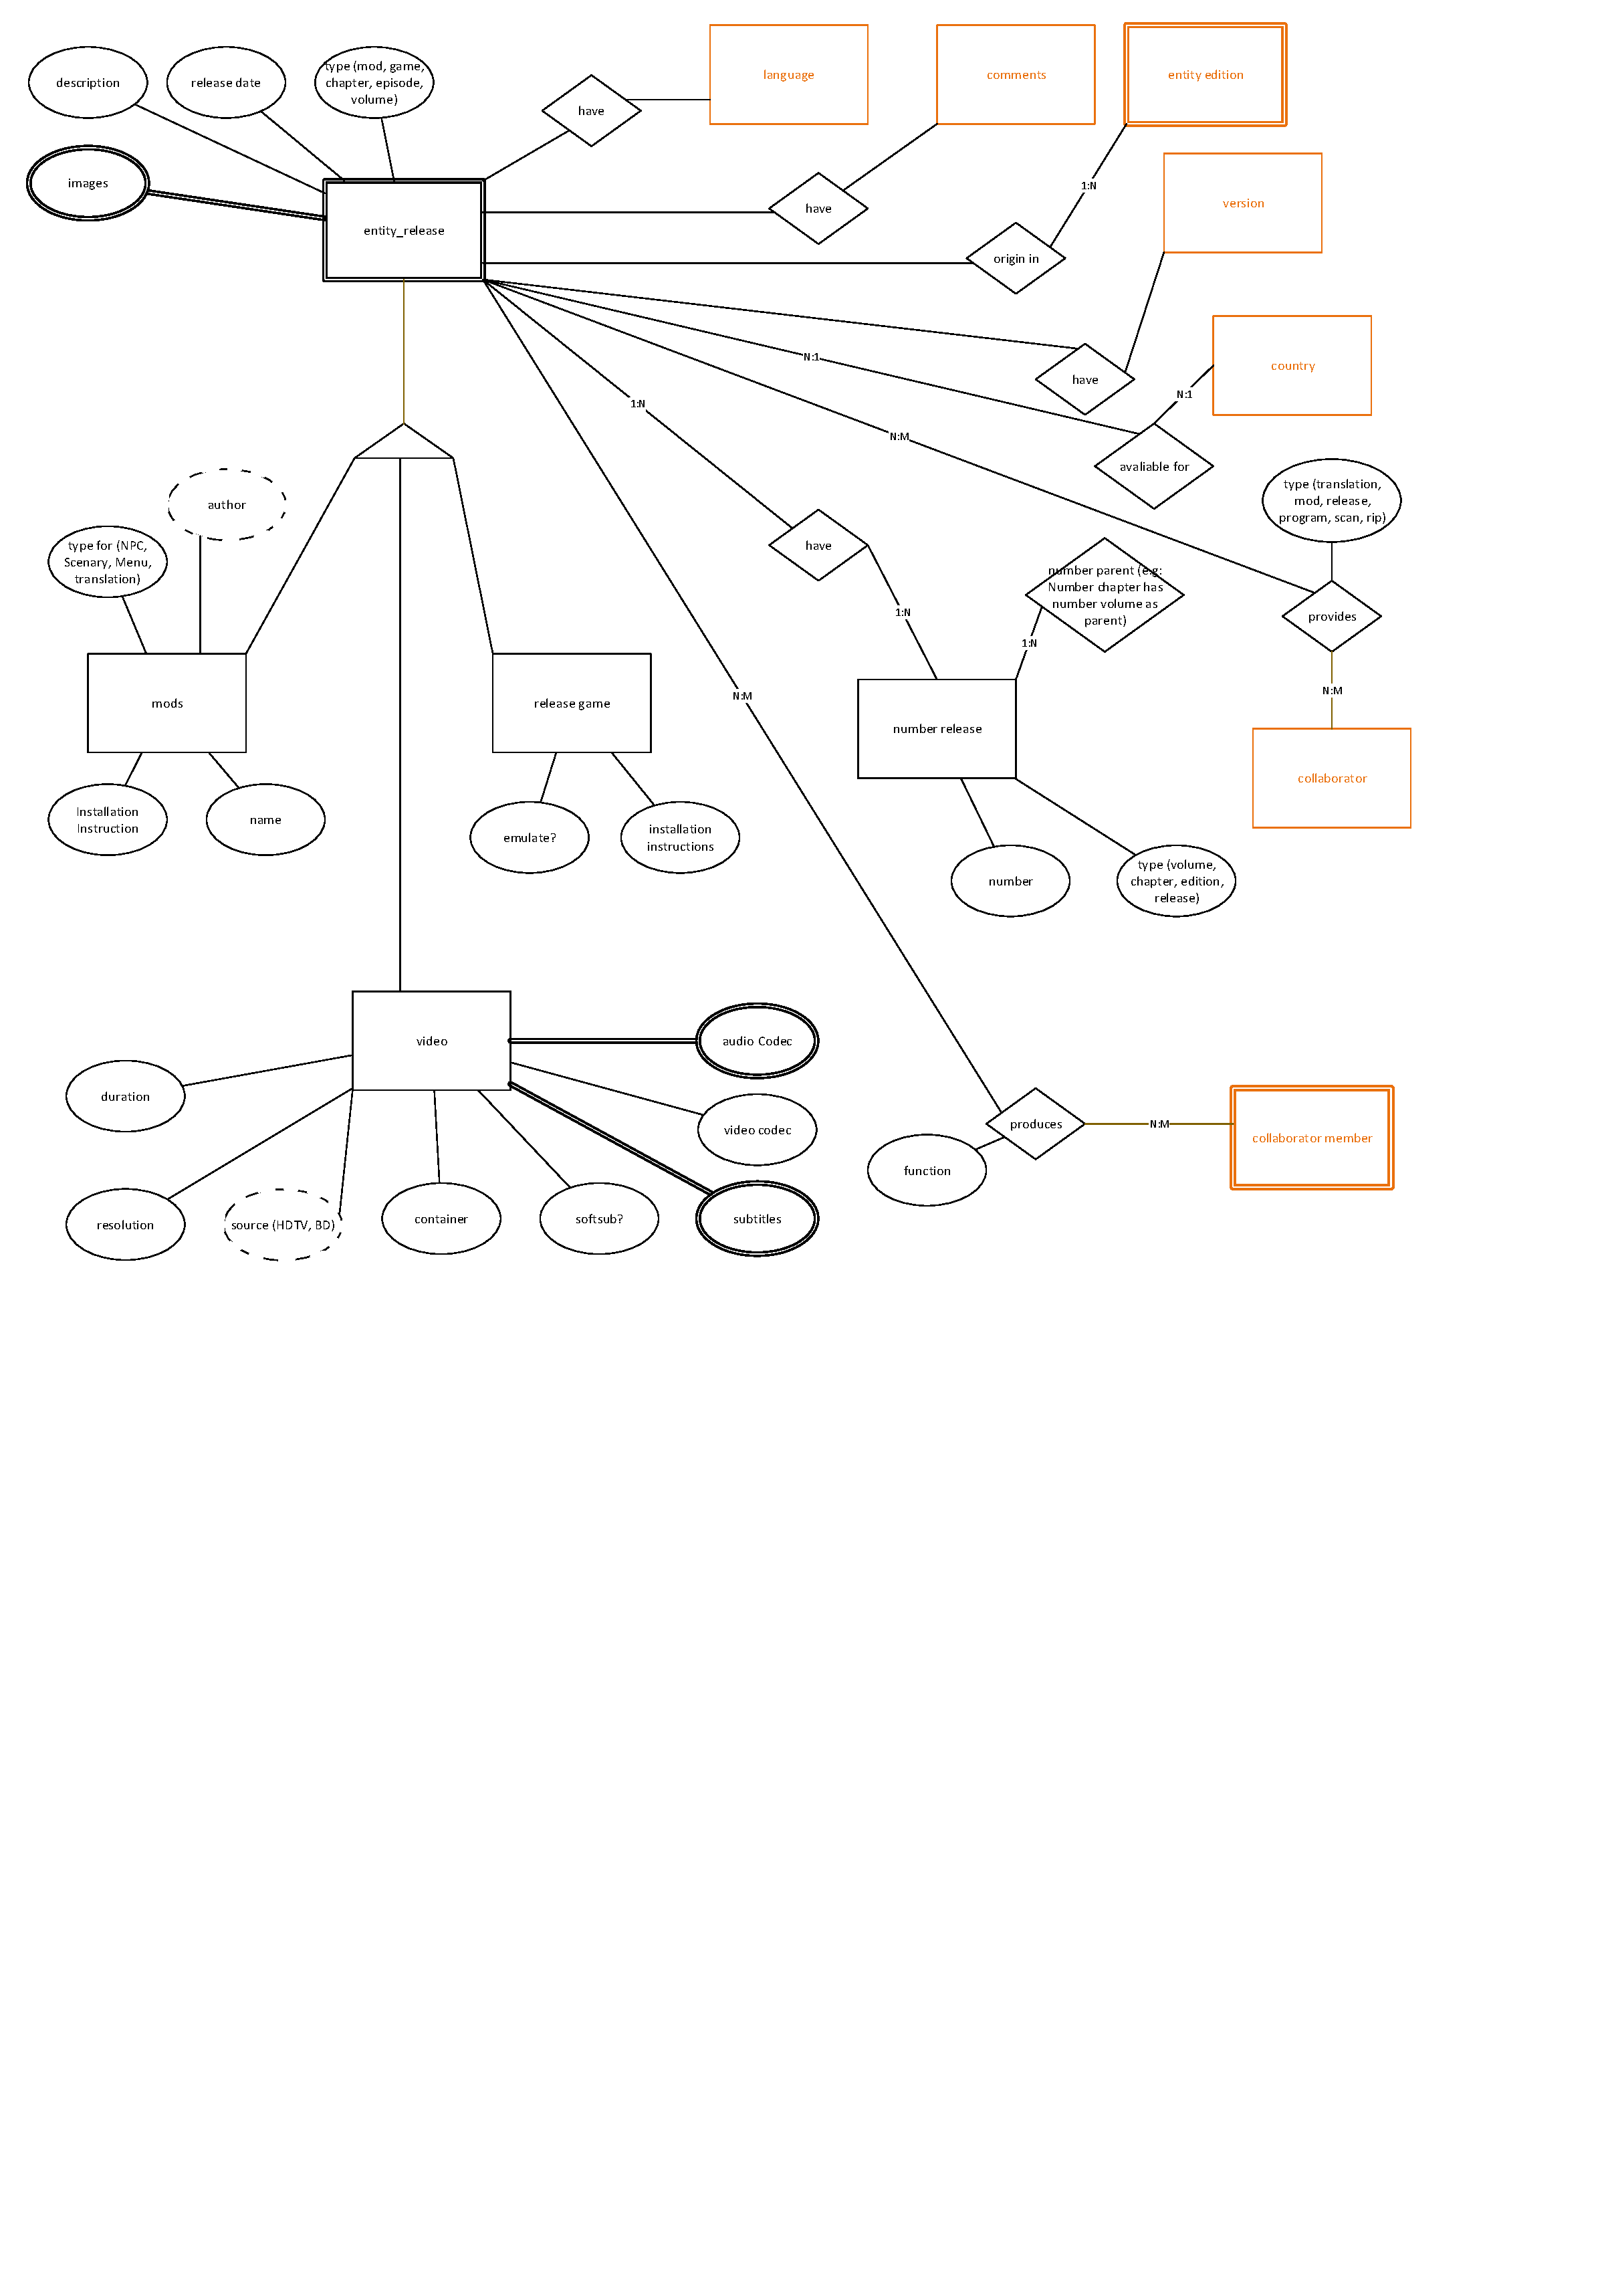
\includegraphics[height=0.8\textheight,width=1.1\textwidth]{MER_-_Release.pdf}
\caption{Entidades responsáveis pelo armazenamento de conteúdo disponibilizado na web como modificações de jogos, conhecidos pela abreviação Mod, de traduções não oficiais de conteúdo ainda não licenciado fora do Japão e de distribuições de conteúdos, legalmente, através da Web.} \label{Release}
\end{figure}

\begin{figure}[H]
\centering
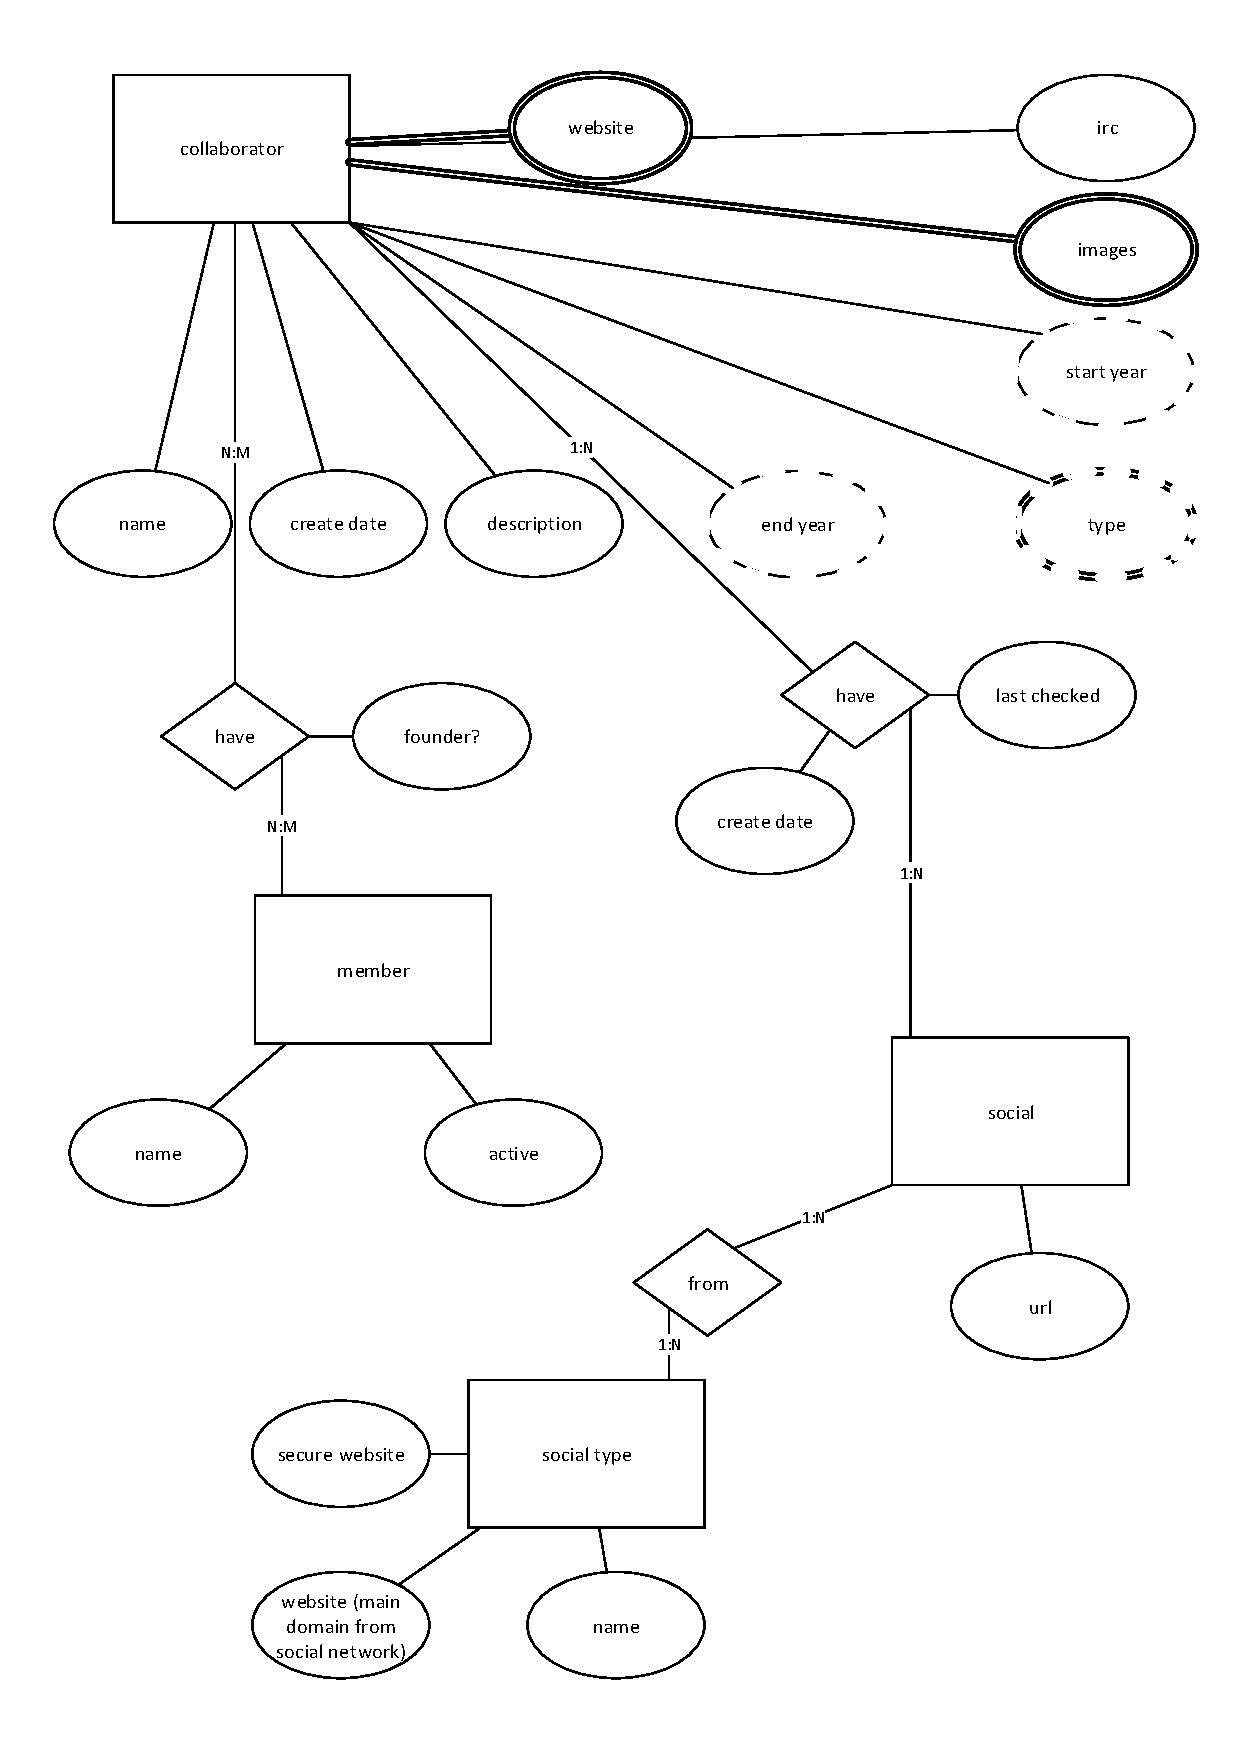
\includegraphics[width=1\textwidth]{MER_-_Collaborator_Social.pdf}
\caption{Entidades com informações sobre grupos de tradução ou distribuidores de conteúdo digital, seus membros e suas redes sociais.} \label{collaborator}
\end{figure}


\begin{figure}[H]
\centering
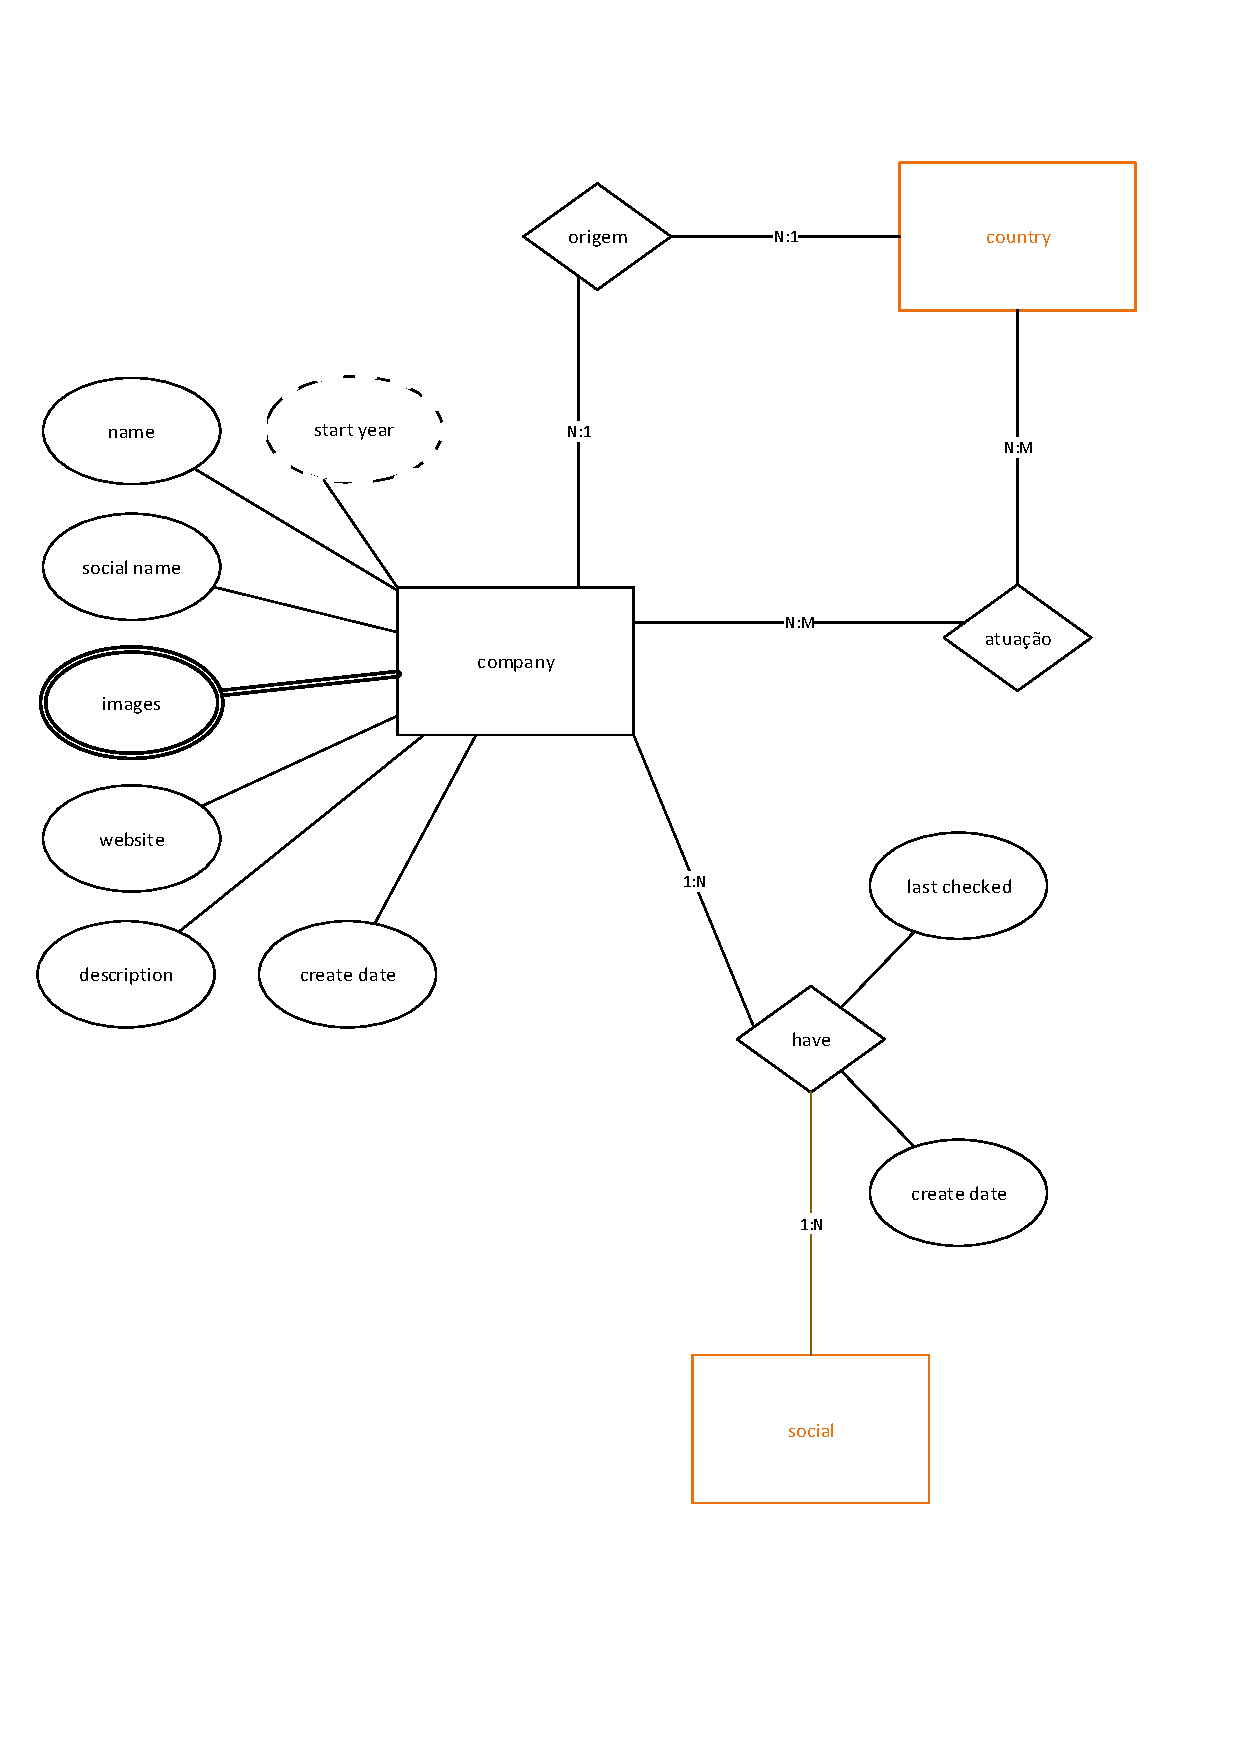
\includegraphics[width=1\textwidth]{MER_-_Company.pdf}
\caption{\textit{Company} é a entidade responsável por armazenar informações de diversas empresas envolvidas na produção de itens. Atributo \textit{images} é utilizado para armazenar apenas a referência das imagens, uma vez que imagens não são armazenadas diretamente no banco de dados.}\label{company}
\end{figure}

\begin{figure}[H]
\centering
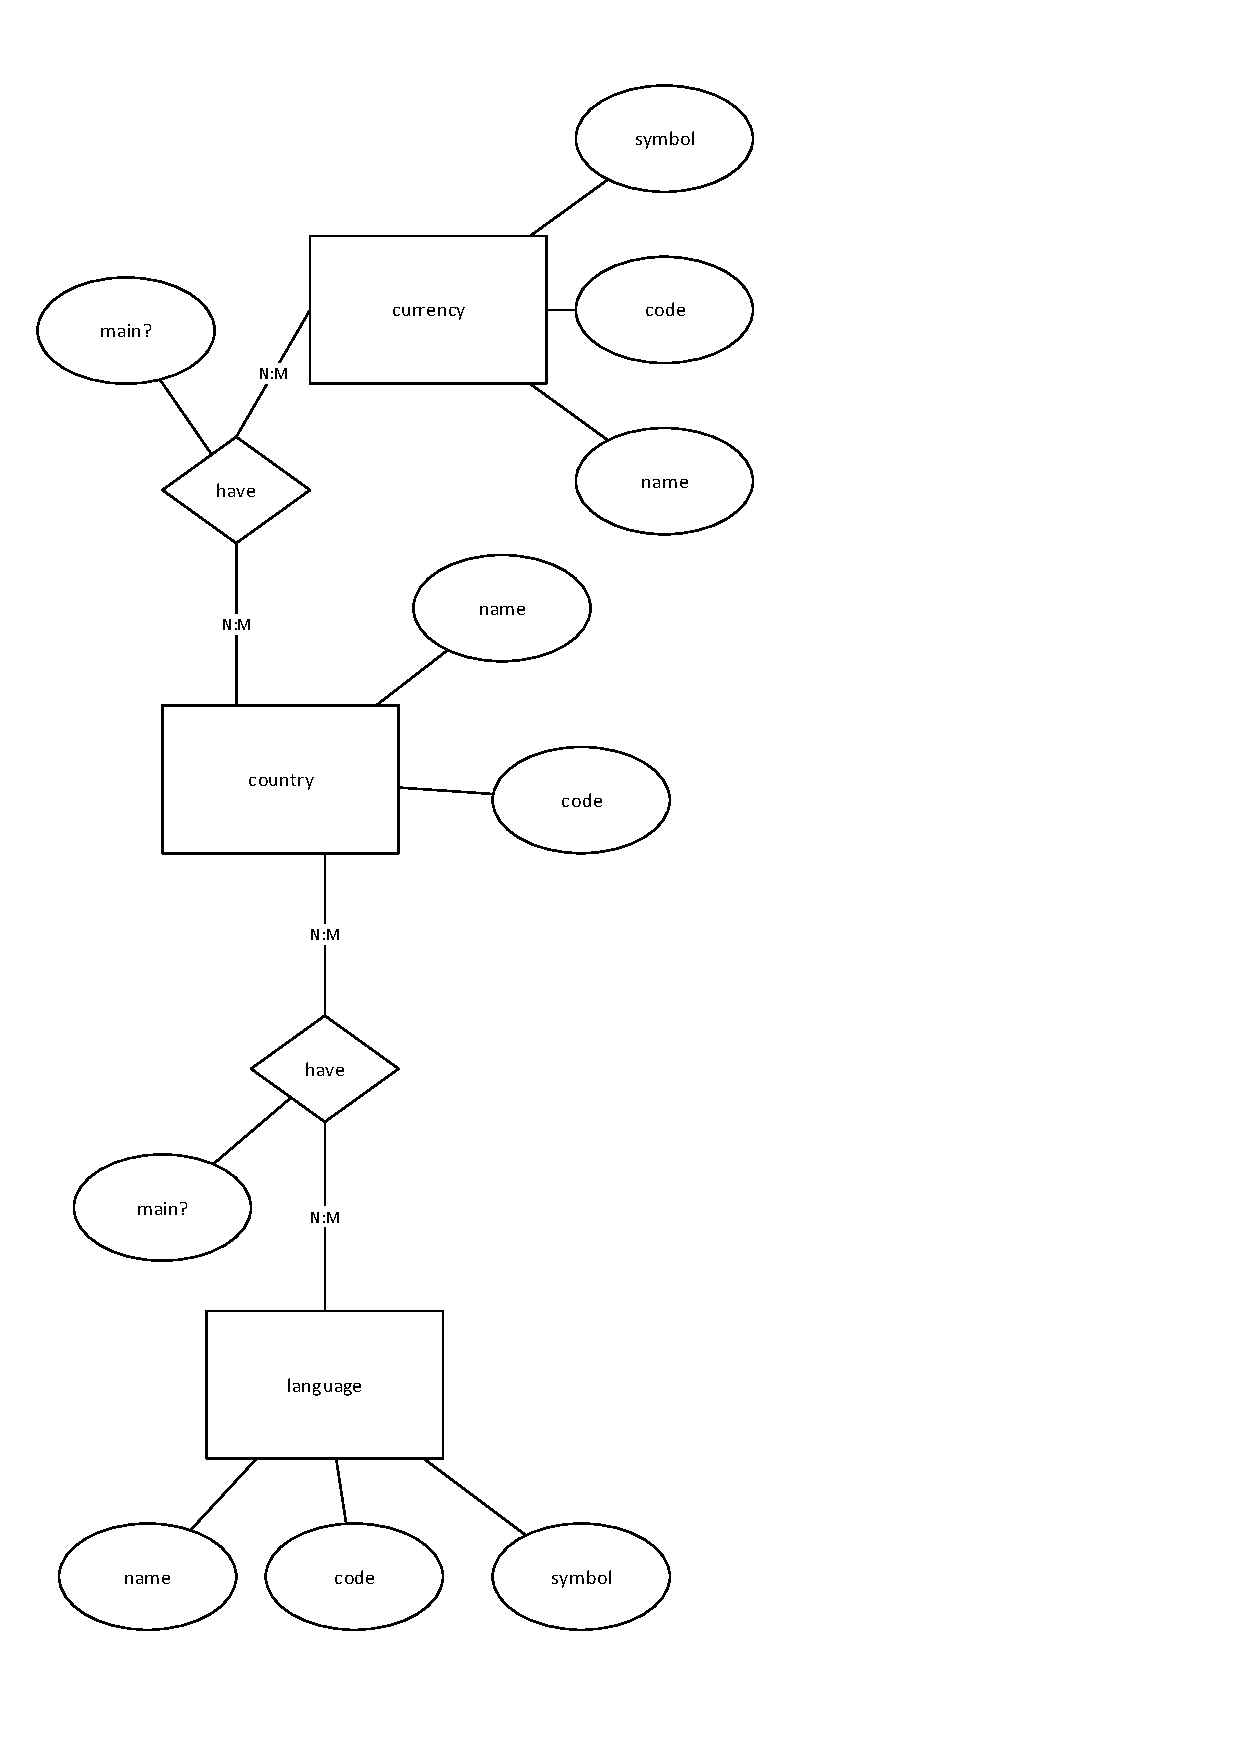
\includegraphics[height=0.92\textheight,width=0.70\textwidth]{MER_-_Country-Language-Currency.pdf}
\caption{Entidades responsáveis pelo armazenamento de informações de países, seus idiomas e suas moedas.} \label{hash}
\end{figure}

\begin{figure}[H]
\centering
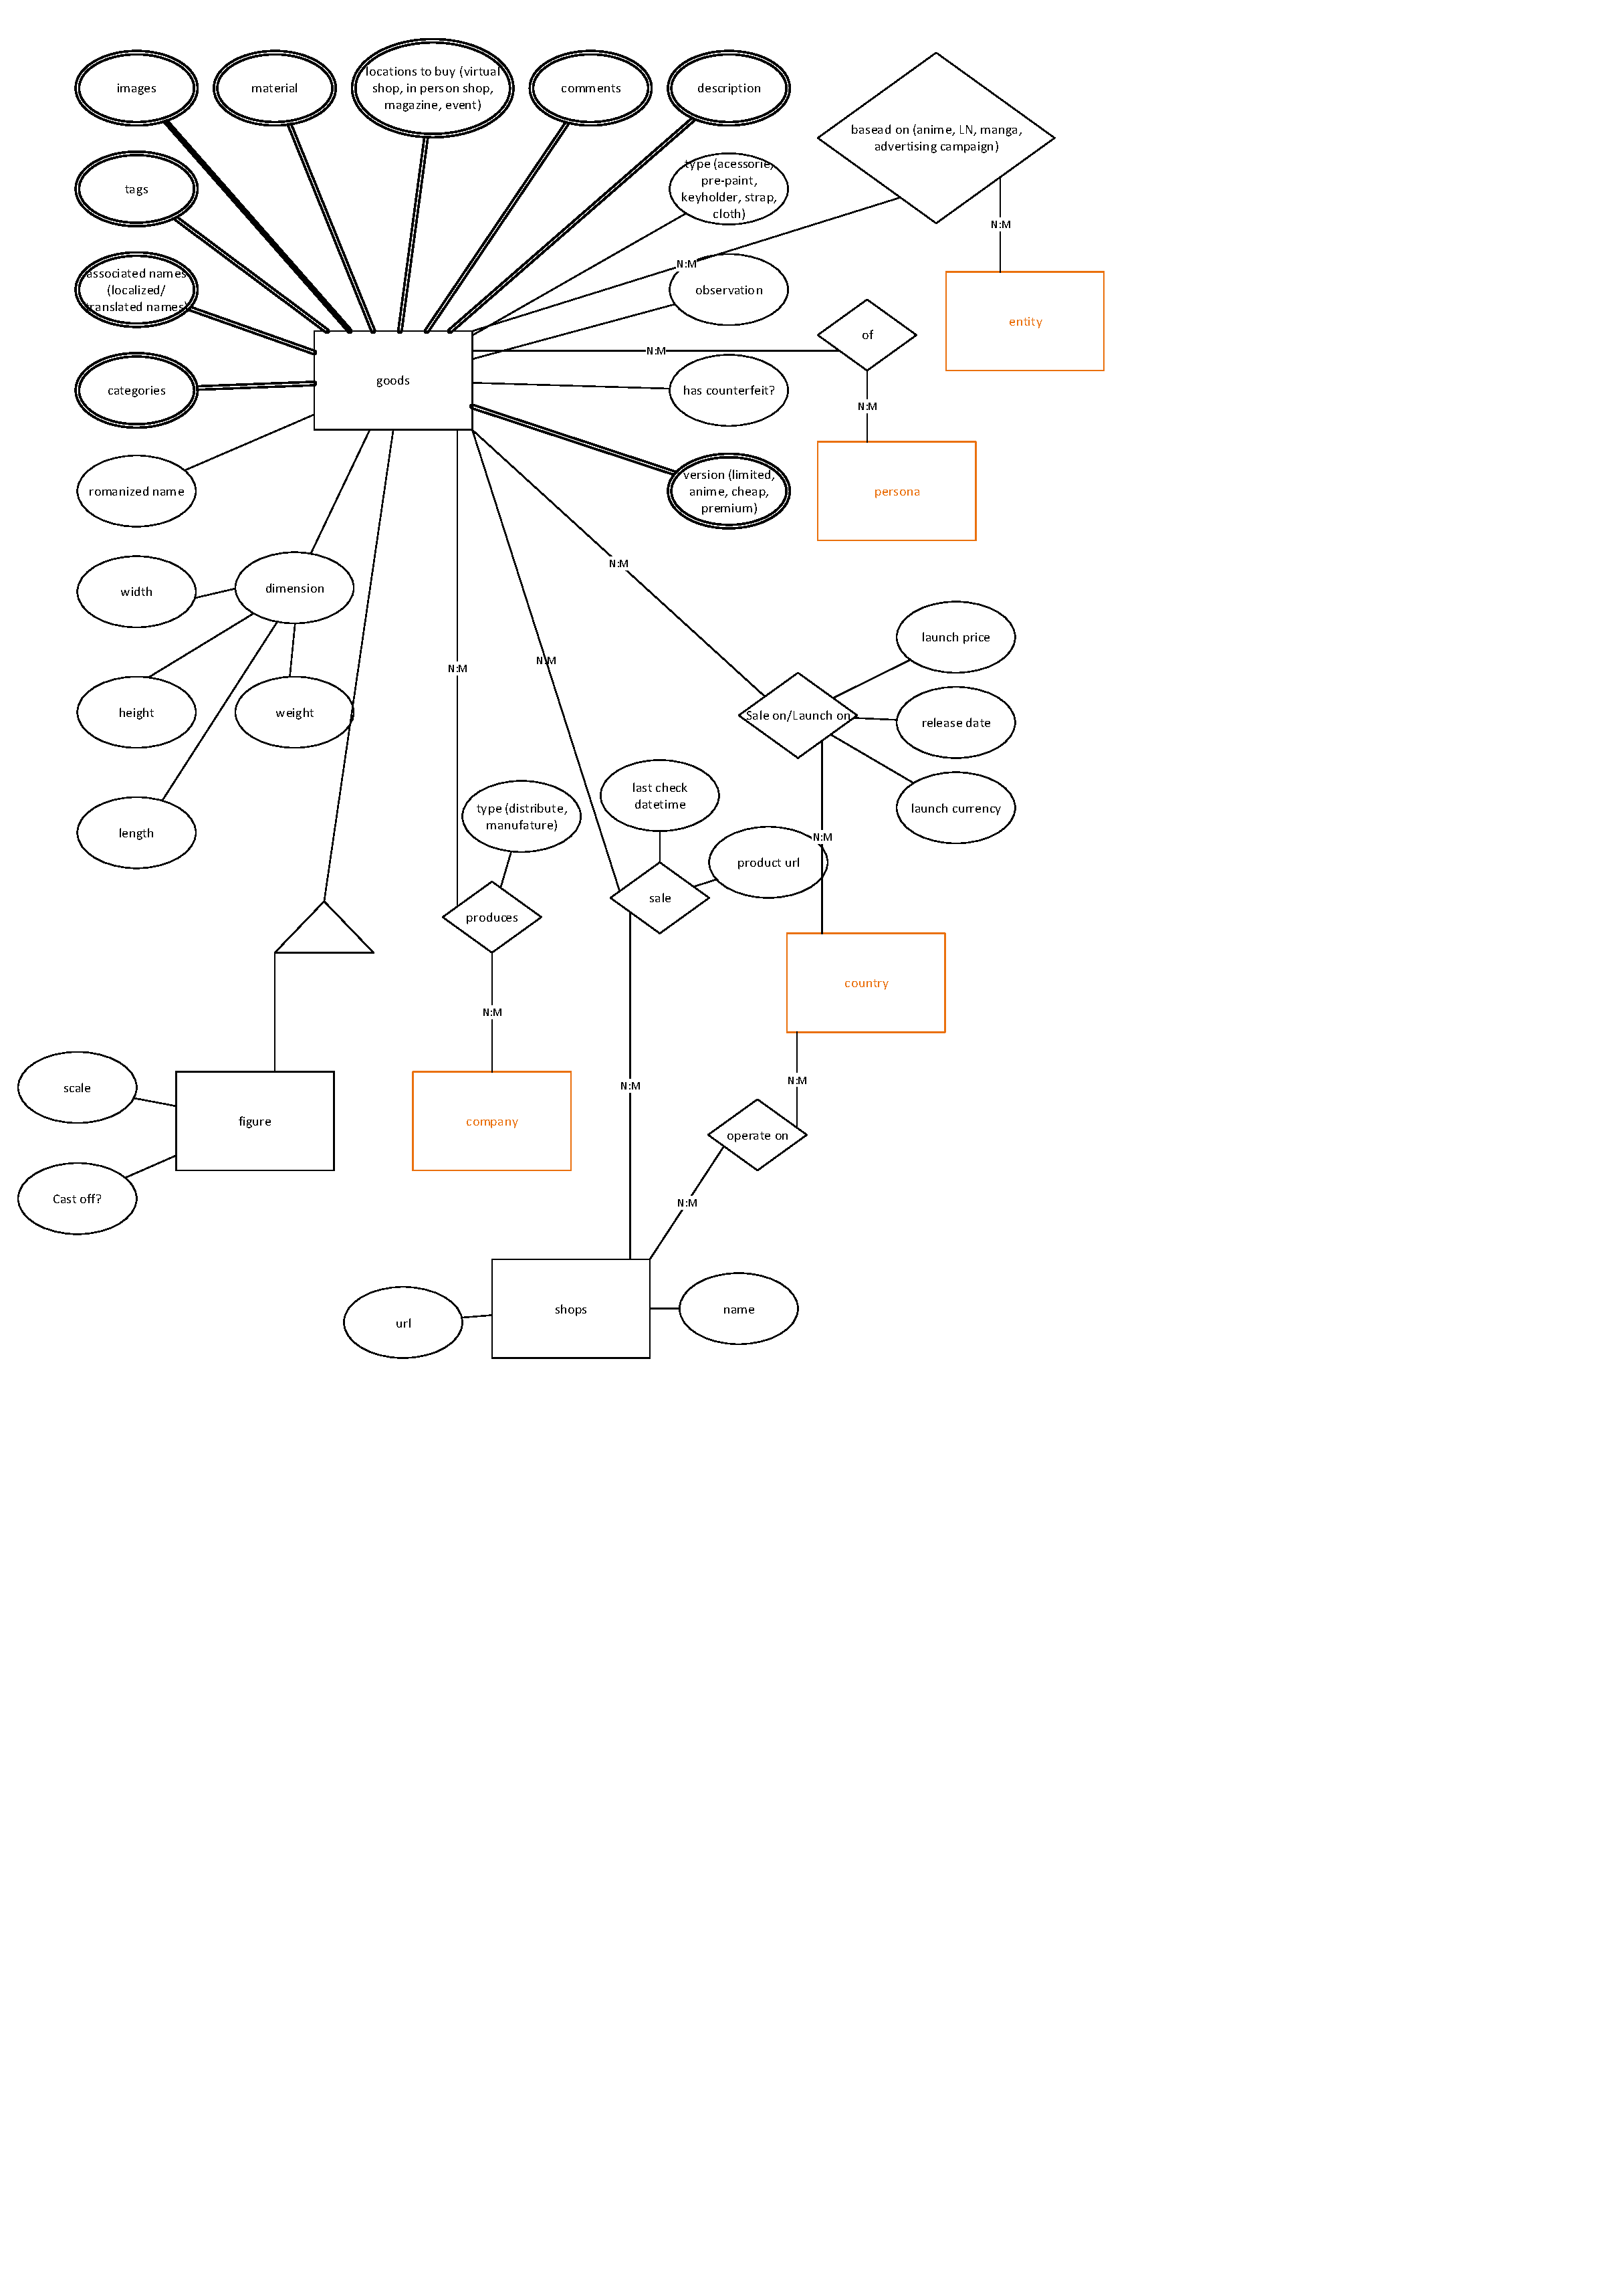
\includegraphics[height=0.98\textheight,width=1.1\textwidth]{MER_-_Goods.pdf}
\caption{Entidade \textit{Goods}, responsável por armazenar dados de produtos, se especializa na entidade \textit{Figure}, responsável por armazenar figuras de ação. Cast-off é o termo utilizado, entre colecionadores, para se referir a opção de remoção de roupa que algumas figuras de ação oferecem.} \label{goods}
\end{figure}

\begin{figure}[H]
\centering
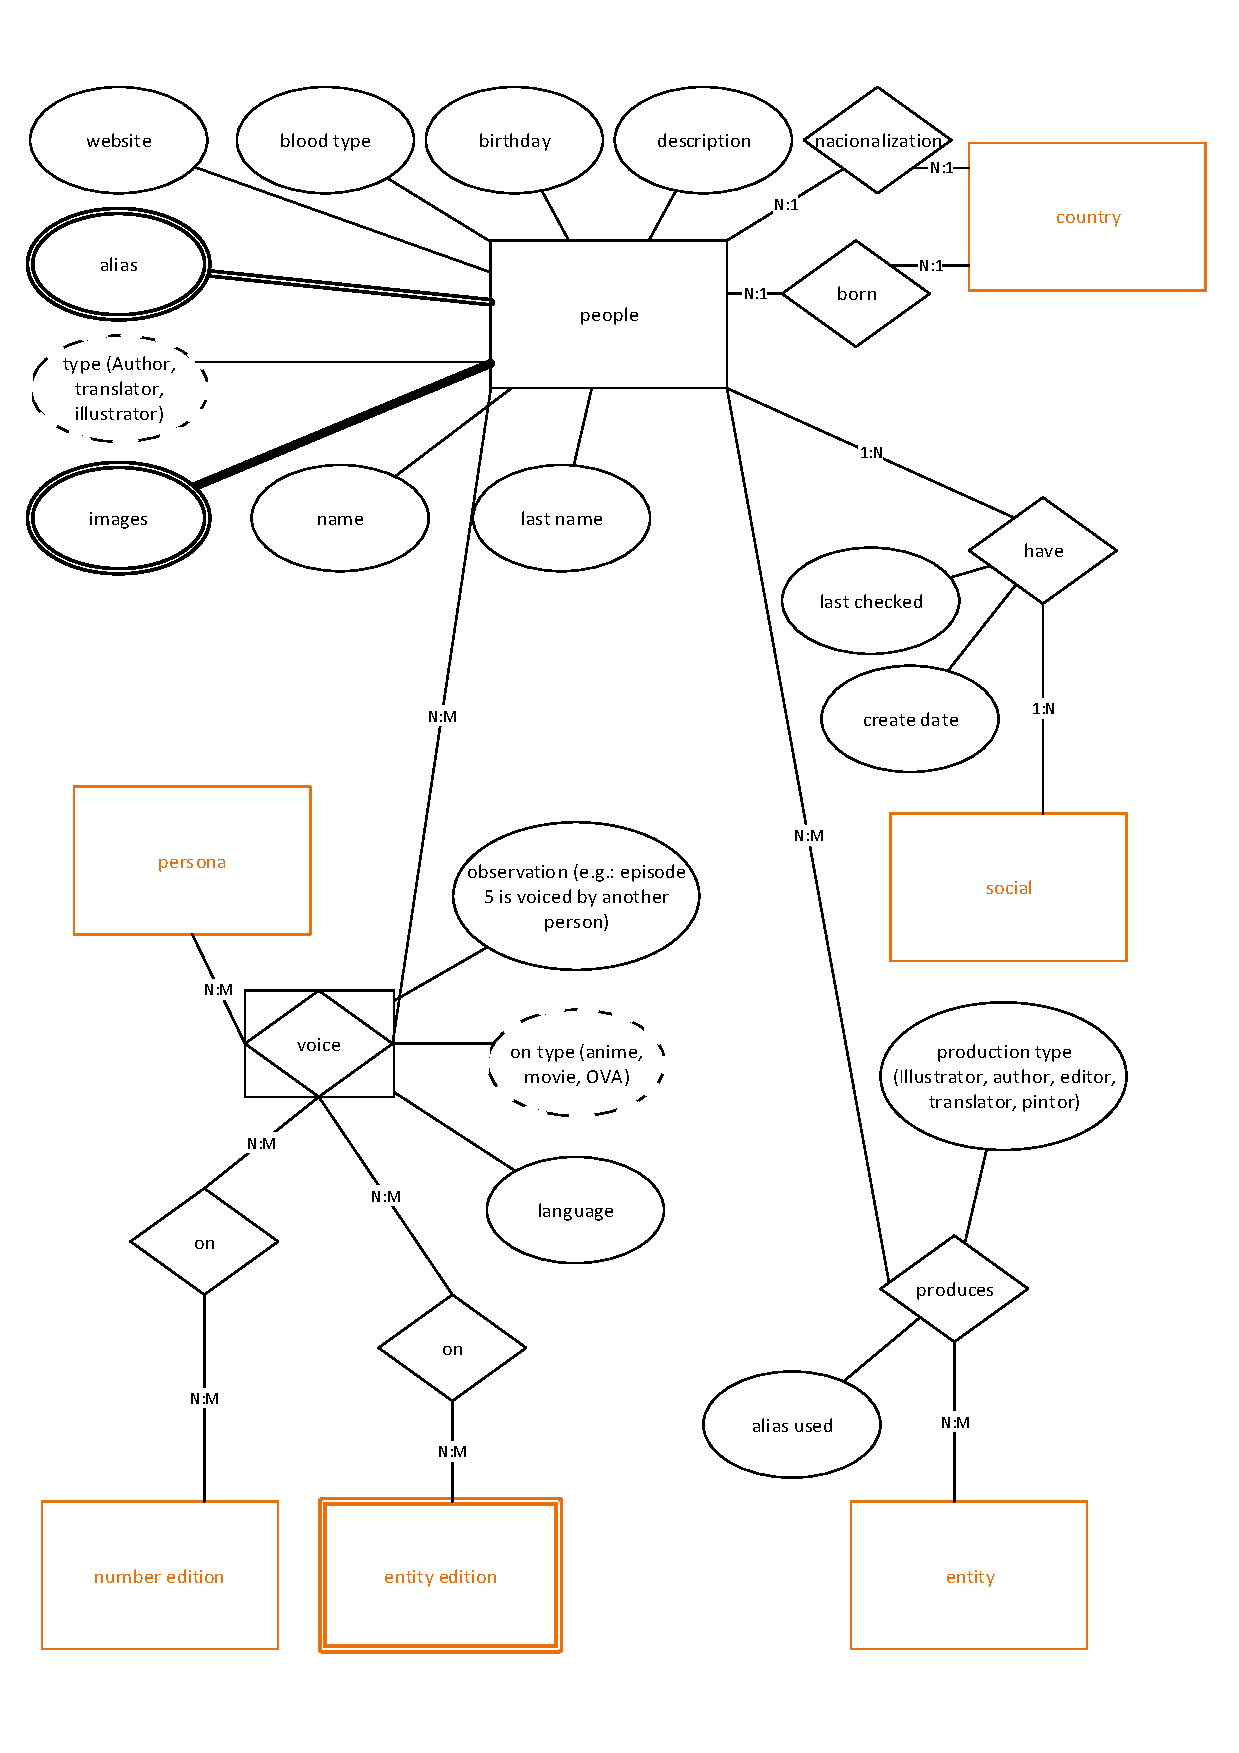
\includegraphics[height=0.92\textheight,width=1\textwidth]{MER_-_People.pdf}
\caption{Entidades responsáveis pelo armazenamento de informações de pessoas envolvidas na produção de itens. Entre o relacionamento de pessoas com personagens há associação utilizada para indicar em quais edições e episódios (\textit{number edition}) o dublador participou. Há situações onde o dublador oficial não pode dublar um episódio ou uma lista de episódios por motivos fora de seu controle.} \label{hash}
\end{figure}

\begin{figure}[H]
\centering
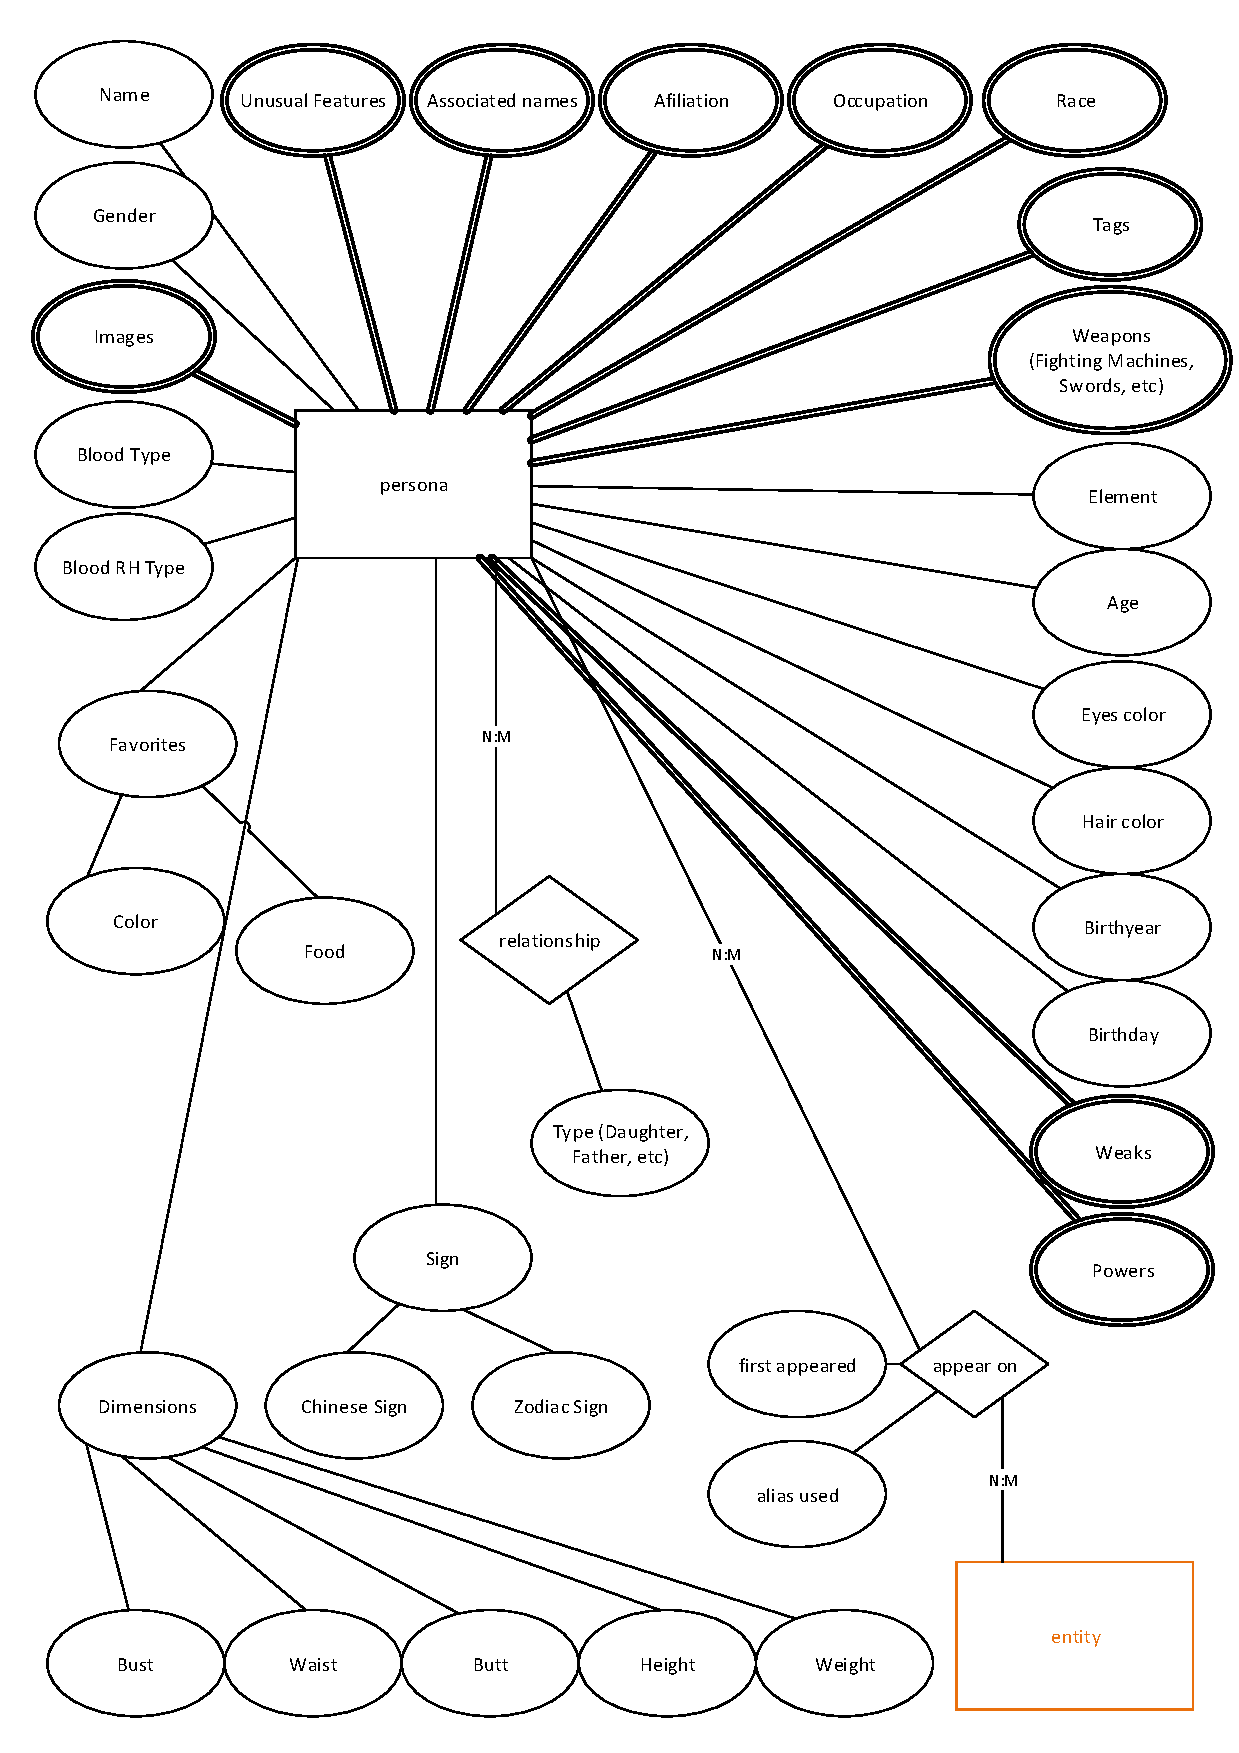
\includegraphics[width=1\textwidth]{MER_-_Persona.pdf}
\caption{Entidade responsável por armazenas personagens e suas características.} \label{Persona}
\end{figure}


\begin{figure}[H]
\centering
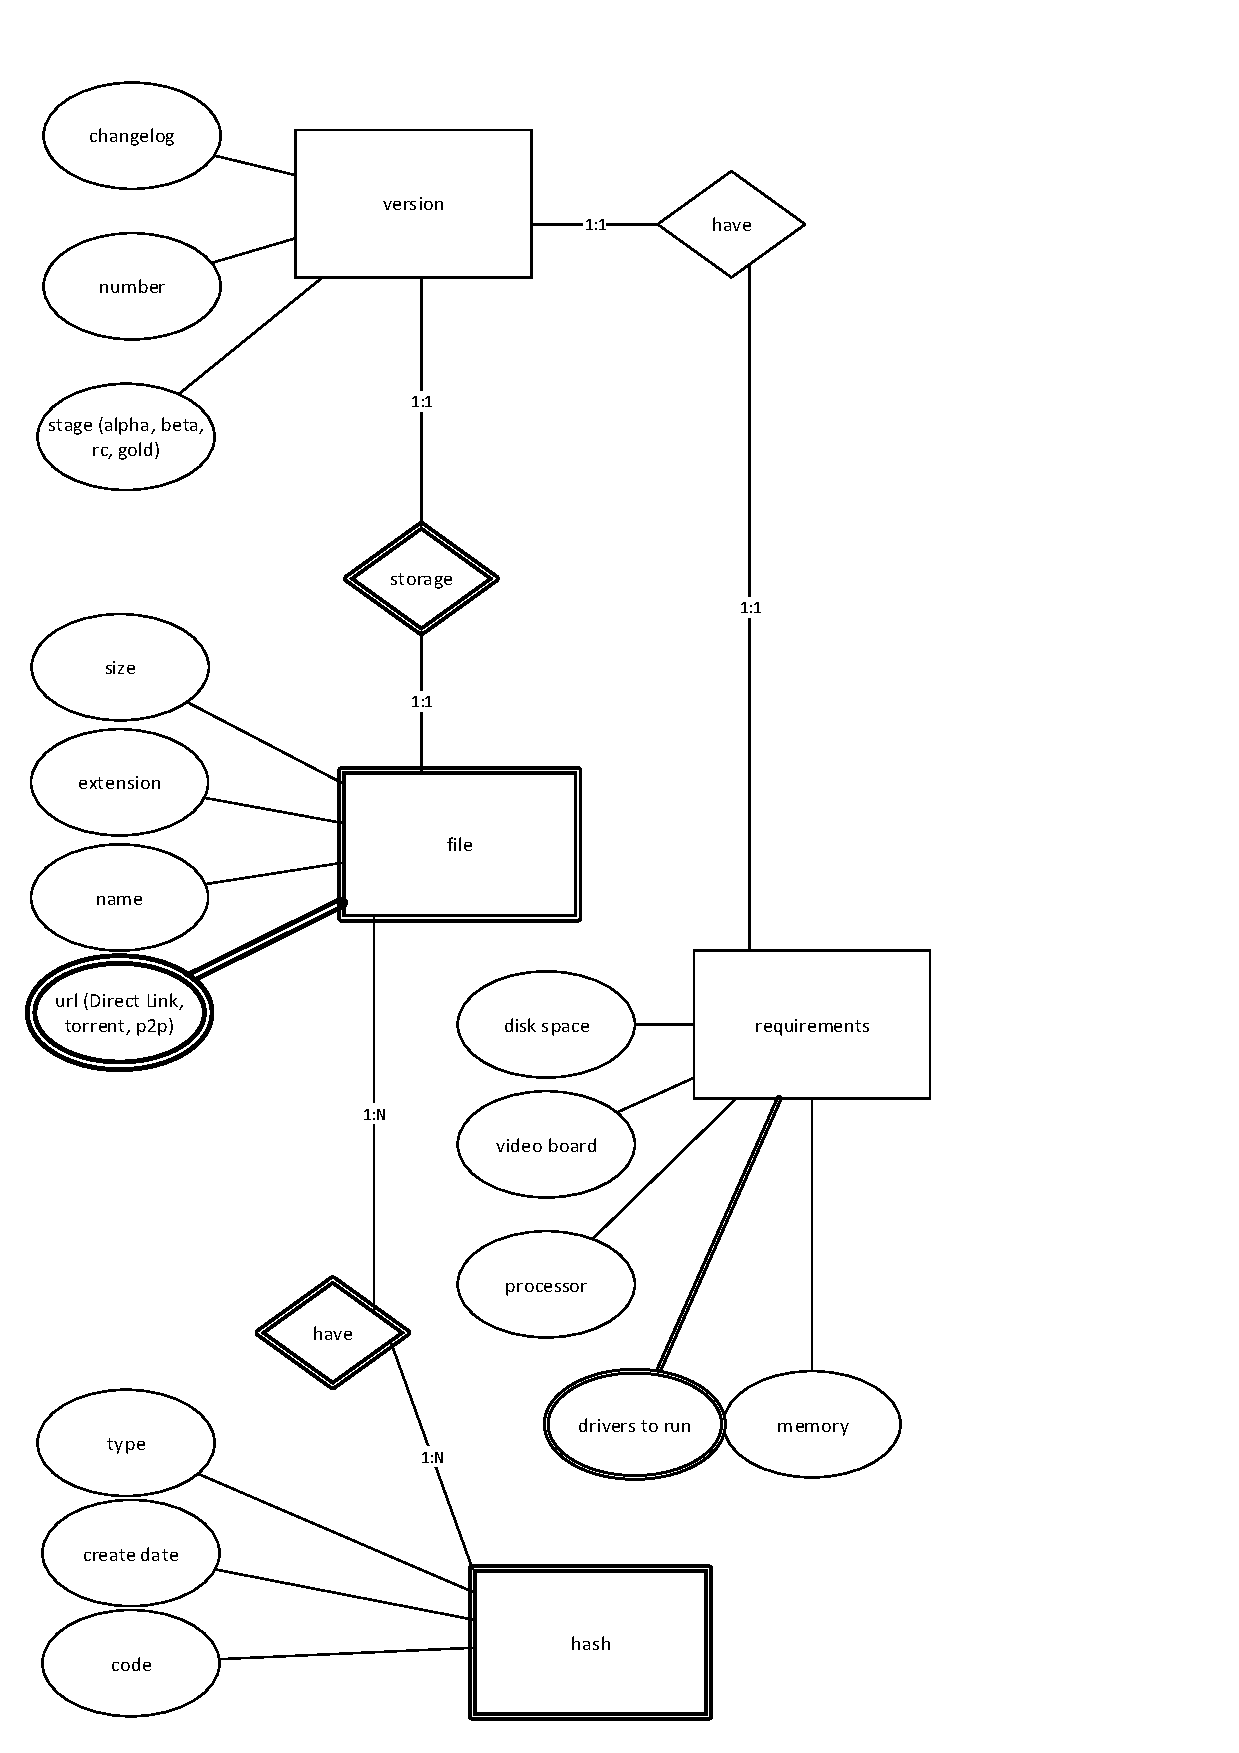
\includegraphics[height=0.95\textheight,width=0.9\textwidth]{MER_-_Version.pdf}
\caption{Entidades responsáveis pelo armazenamento de informações de versões existentes de softwares, animações e livros e seus respectivos arquivos disponibilizados na Web.} \label{hash}
\end{figure}


\begin{figure}[H]
\centering
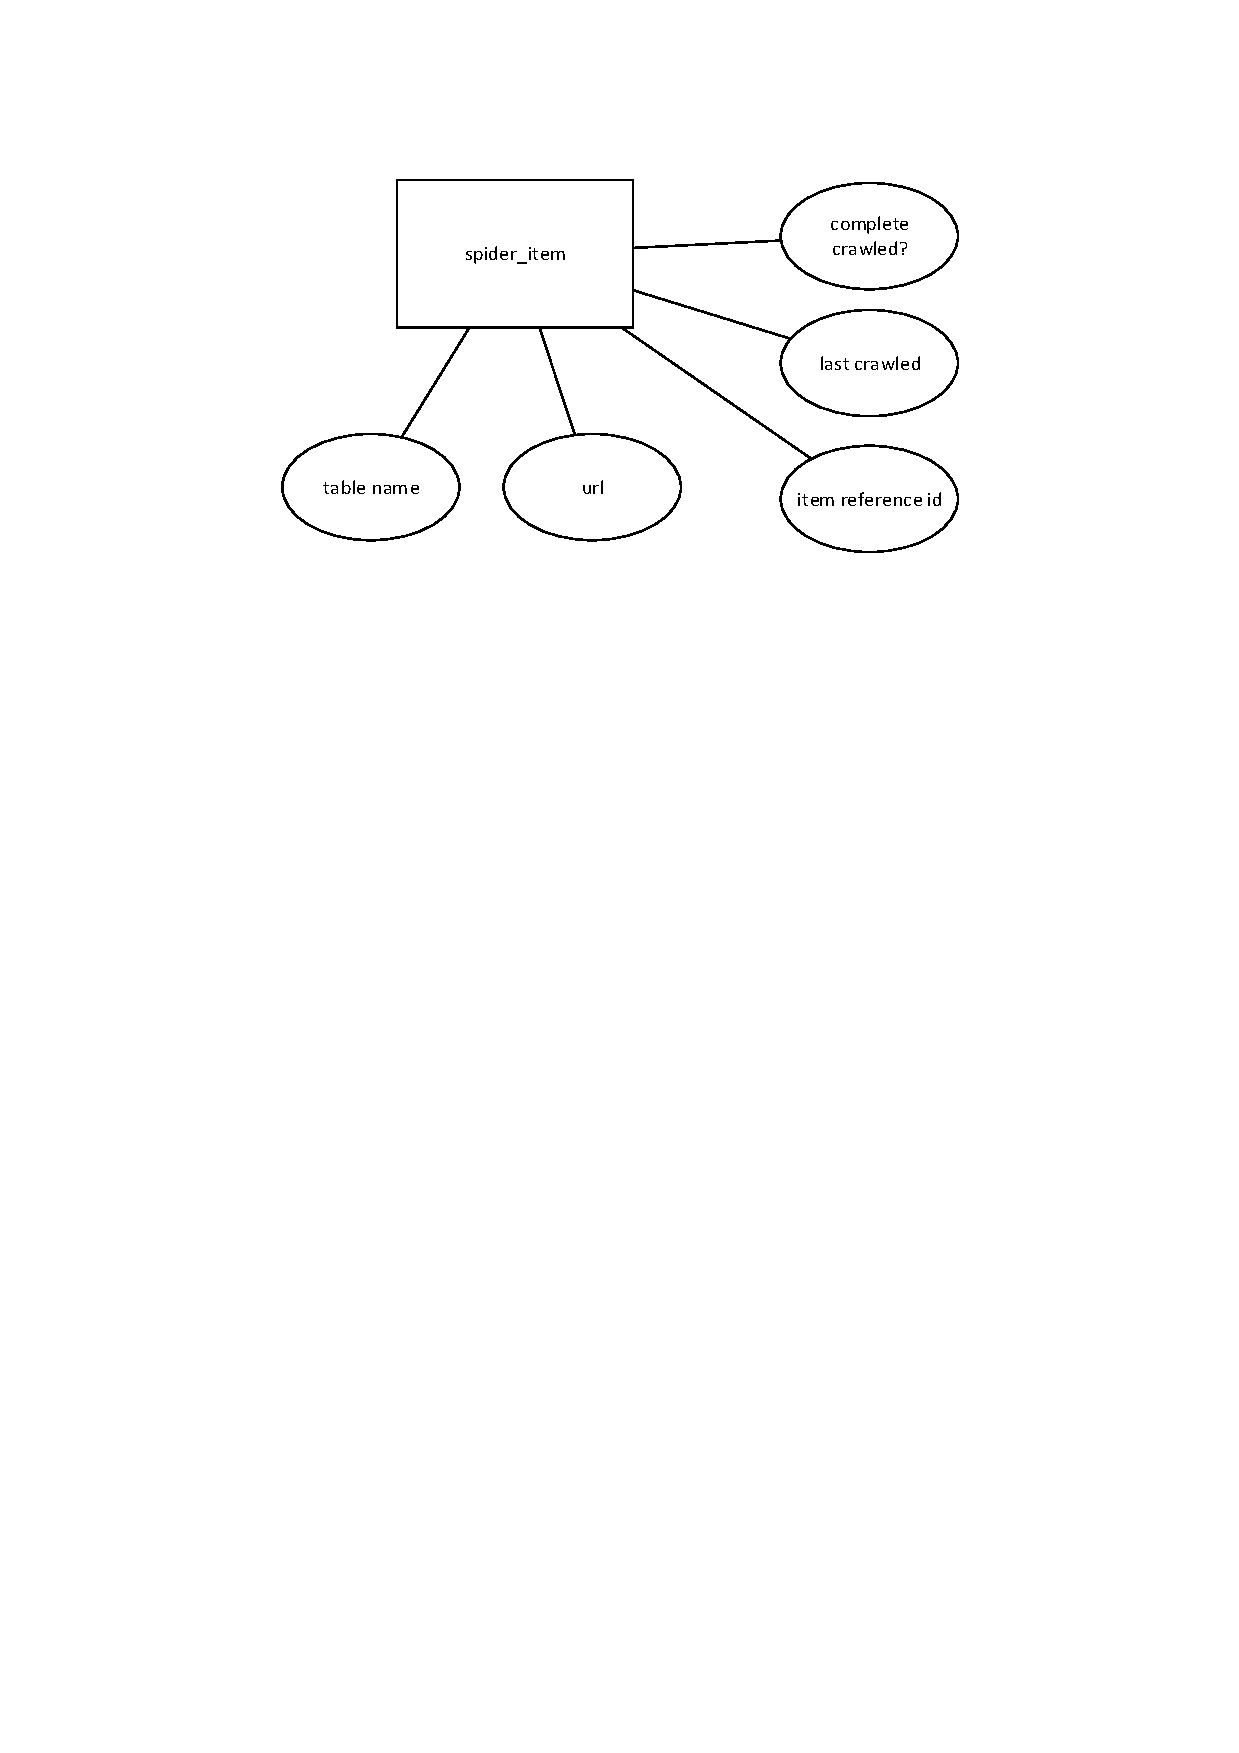
\includegraphics[width=1\textwidth]{MER_-_Spider_item.pdf}
\caption{Entidade responsável pelo armazenamento das URLs que tiveram informações extraídas e salvas no banco de dados. Essa entidade não é utilizada para verificar se uma URL já foi visitada durante uma execução do Crawler, isso é feito no próprio Crawler. Essa entidade serve para garantir que cada URL não salve informações duplicadas em multiplas execuções do Crawler, por isso é salvo a referência do ID e a tabela em que a informação foi salva. É permitido que alguns dados duplicados sejam salvos, por exemplo títulos, para casos em que itens diferentes possuam o mesmo nome.} \label{hash}
\end{figure}

\subsubsection{Modelo Relacional}

Após a criação do Modelo Conceitual foram criadas as tabelas e relacionamentos do Modelo Relacional seguindo as três Formas Normais, separando portando atributos multi-valorados, não relacionados a totalidade da chave primaria em tabelas próprias quando necessário.

Também foram criadas chave-primarias não naturais, como índices numéricos que são auto incrementados na inserção de conteúdo, e foram definidos valores padrão para atributos que armazenam Data e Hora.

Para as entidades que possuem mais de um tipo de título ou descrição, como \textit{Entity}, \textit{Persona} e \textit{People} que possuem o título principal e título, foram criadas entidades para armazenamento desses títulos ou descrições com um atributo que identifica também o idioma do texto.


\subsubsection{Ferramentas Utilizadas para Modelagem}

\paragraph{Modelo Conceitual\newline}

Para a modelagem do Banco de Dados e criação do Modelo Conceitual foi escolhido o Microsoft Visio que permite a geração de diversos tipos de diagramas, possibilitando a criação de novos itens se necessários para uso nos diagramas. Alguns dos itens como Associação e Atributos Compostos não estão presentes por padrão na modelagem de dados que vem com o Microsoft Visio e tiveram que ser criadas.

\begin{figure}[H]
\centering
\mbox{\subfigure{
\includegraphics[width=1in]{Generalization.pdf}}\quad
\subfigure{
\includegraphics[width=1in]{attribute-derivate.pdf} }\subfigure{
\includegraphics[width=1in]{attribute-generalization.pdf} }}
\caption{Objetos que precisaram ser criados: associação (a), atributo derivado (b) e generalização/especialização (c).}
\label{fig6}
\end{figure}

\paragraph{Modelo Relacional\newline}

Para o Modelo Relacional foi utilizado o DBDesigner na sua 4ª versão, que permite a migração do Modelo Relacional para código SQL do MySQL. DBDesign não oferece suporte ao PostgreSQL sendo necessário para criação do Modelo Lógico algumas alterações no arquivo SQL. 

Para um Modelo Relacional extenso o DBDesigner porém se mostrou limitado ao não permitir o aumento na área útil em que as entidades poderiam ser adicionadas. Para uma modelagem extensa como a do banco de dados desse projeto essa limitação dificultou a organização pela falta de espaço fazendo com que as entidades ficassem muito próximas umas das outras. 

Além dessa limitação a execução da máquina virtual do JAVA (JVM) para o DB Design apresenta problemas com a hibernação no Sistema Operacional Windows, quando se retorna de uma hibernação, com a JVM ativa, ao tentar salvar ou exportar um arquivo no DBDesign o programa trava sendo necessário reniciar o computador para voltar a utilizar essas opções. Portanto não é recomendo o uso do DB Design para um modelo relacional extenso. 

\textbf{Modelo Lógico}\newline

Para execução do Modelo Lógico foi utilizado o PostgreSQL 9.3 e o PgAdmin III para o sistema operacional Windows 8. 

Por padrão o usuário inicial no PgAdmin III é o postgres, mas para execução de queries de seleção, inserção e atualização foi criado outro usuário para uso no nosso sistema crawler. 

\subsubsection{Detalhes da Implementação do Modelo Lógico}

Ao exportar o arquivo SQL do DBDesigner é criado código SQL especificamente para MySQL, portanto para usarmos no PostgreSQL esse código precisou ser alterado.

O código SQL resultante do DB Design possui a criação de índices e chaves-estrangeiras inclusas na criação da própria tabela. Apesar de ser compatível com o PostgreSQL resolvemos separar esse código em outros arquivos para uma melhor organização.

No MySQL chave-primárias sequenciais são definidas como valor numérico com propriedade \emph{auto\_increment}. Como \emph{auto\_increment} não está disponível para o PostgreSQL usamos o equivalente SERIAL.

Código MySQL:

id integer primary key auto\_increment

Equivalente em PostgreSQL:

id serial

Outra própriedade presente no código MySQL que não está disponível em PostgreSQL é o DATETIME, usado para armazenar data e hora. Uma alternativa adotada foi utilizar timestamp, que também armazena data e hora, pórem em microsegundos desde o epoch Unix (01/01/1970 00:00). Para inserção do timestamp, além de ser aceito o tempo em microsegundos, se fornecidade string concatenada de data e hora no padrão 'AAAA-MM-DD HH:MM:SS' o PostgreSQL fará a conversão automaticamente para microsegundos. 

No PostgreSQL há dois tipos de timestamp: com fuso horário e sem fuso horário. Para salvar timestamps que não possuam um fuso horário ainda determinado, é indicado o uso de timestamp sem fuso horário. Nesse projeto foi escolhido usar timestamp com fuso horário para indicar quando alguns dados foram inseridos.

Código MySQL:

\begin{lstlisting}[language=SQL,morekeywords={now(),DATETIME}]
data_cadastro DATETIME NOT NULL DEFAULT now()
\end{lstlisting}

Alternativa em PostgreSQL:

\begin{lstlisting}[language=SQL,morekeywords={now(),without}]
data_cadastro timestamp without time zone NOT NULL DEFAULT
now()
\end{lstlisting}

Um recurso presente em PostgreSQL é a herança entre tabelas, que permitem que tabelas herdem atributos não-chave de outras tabelas. Usamos esse recurso em entidades que possuem especialização, como as entidades \textit{goods} e \textit{edition}. Como herança não é um recurso presente no MySQL durante a criação do Modelo Relacional no DB Design foi utilizado relacionamento de cardinalidade 1:1 entre as tabelas que sofrem especialização/generalização.

O PostgreSQL em sua versão estável mais recente, 9.3, ainda não oferece criação automatizada de relacionamentos e unicidade entre tabelas pais e descendentes quando se indica uma herança na tabela descendente. Atributos chaves-estrageira usados na tabela pai, que também devem estar presentes na tabela descendente, precisam ser inclusos manualmente.

Código para criação de tabela com herança em PostgreSQL:

\begin{lstlisting}[language=SQL,morekeywords={now(),without}]

CREATE TABLE figure (
    ...
) INHERITS (goods);
\end{lstlisting}

Uma pesquisa no banco de dados PostgreSQL efetuada em uma tabela pai automaticamente inclui resultados presentes nas tabelas descendentes. Para evitar esse comportamento é necessário indicar que se deseja procurar apenas na tabela pai. Isso pode ser indicado utilizando ONLY antes do nome da tabela no código SQL de consulta.

Código de consulta em PostgreSQL com ONLY:

\begin{lstlisting}[language=SQL,morekeywords={only}]
SELECT * FROM ONLY goods;
\end{lstlisting}

\subsection{Crawler}

Um crawler é um programa que visita websites, segue links e extrai dados de páginas especificas. Um crawler deve a partir de uma URL inicial seguir recursivamente todas as URLs acessíveis a partir da inicial. Critérios podem ser utilizados para indicar quais URLs seguir, como por exemplo o critério de considerar apenas o domínio atual do site, excluindo websites externos de publicidade e redes sociais.

Na execução inicial o Crawler faz o download do código HTML da página da URL inicial e extrai a informação "href" das tags $<$a$>$ presente na página e as coloca numa lista de processamento usada na analise que determina se a URL deve ser seguida, extraída ou removida da lista. 

Para evitar o problema de loops infinitos, por exemplo, quando uma página A possui um link para uma página B e a página B possui link para a página A, deve-se criar uma lista de URLs já visitados para verificação. Esse problema não necessáriamente ocorre em uma página imediata a outra, podendo ocorrer mais tarde durante a execução do crawler.  

\begin{figure}[H]
\centering
\mbox{\subfigure{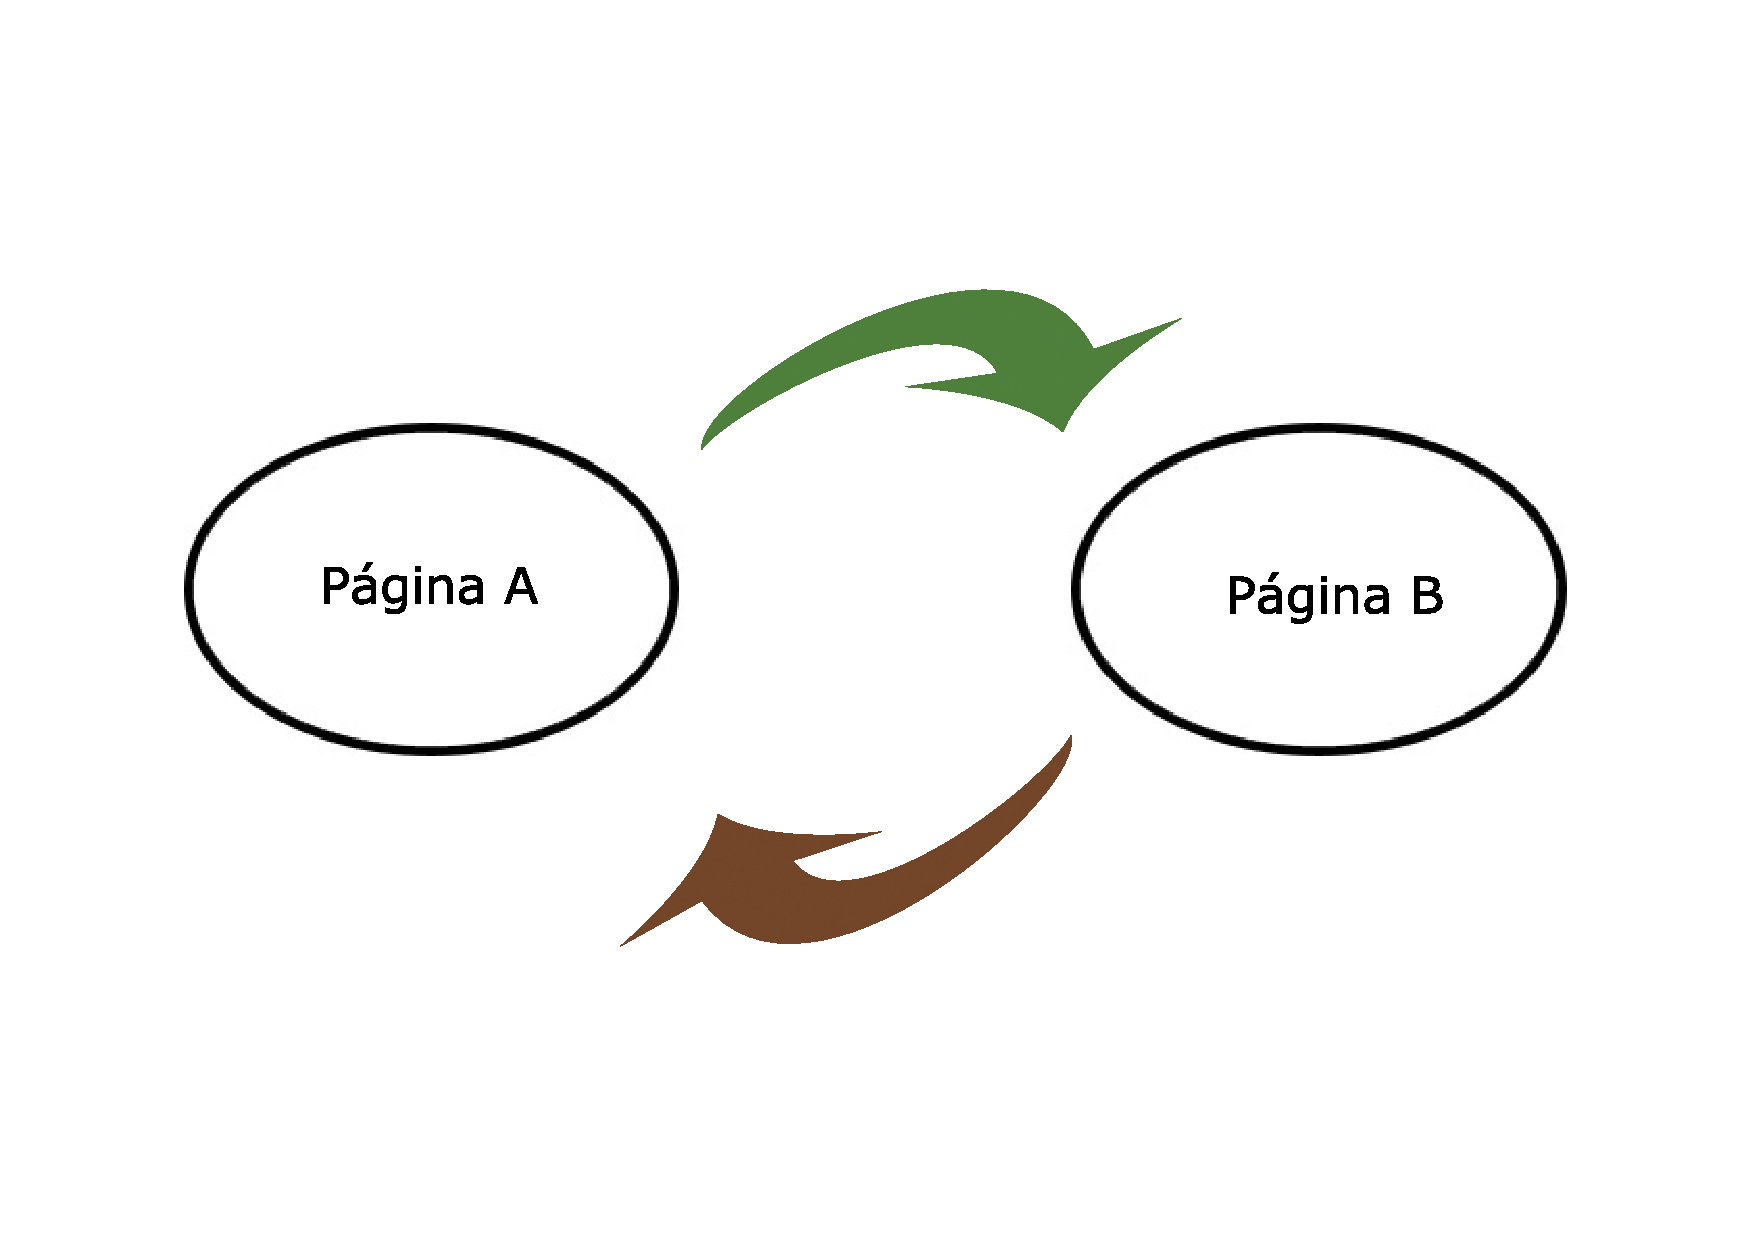
\includegraphics[width=2.5in]{loop1.pdf}}\quad
\subfigure{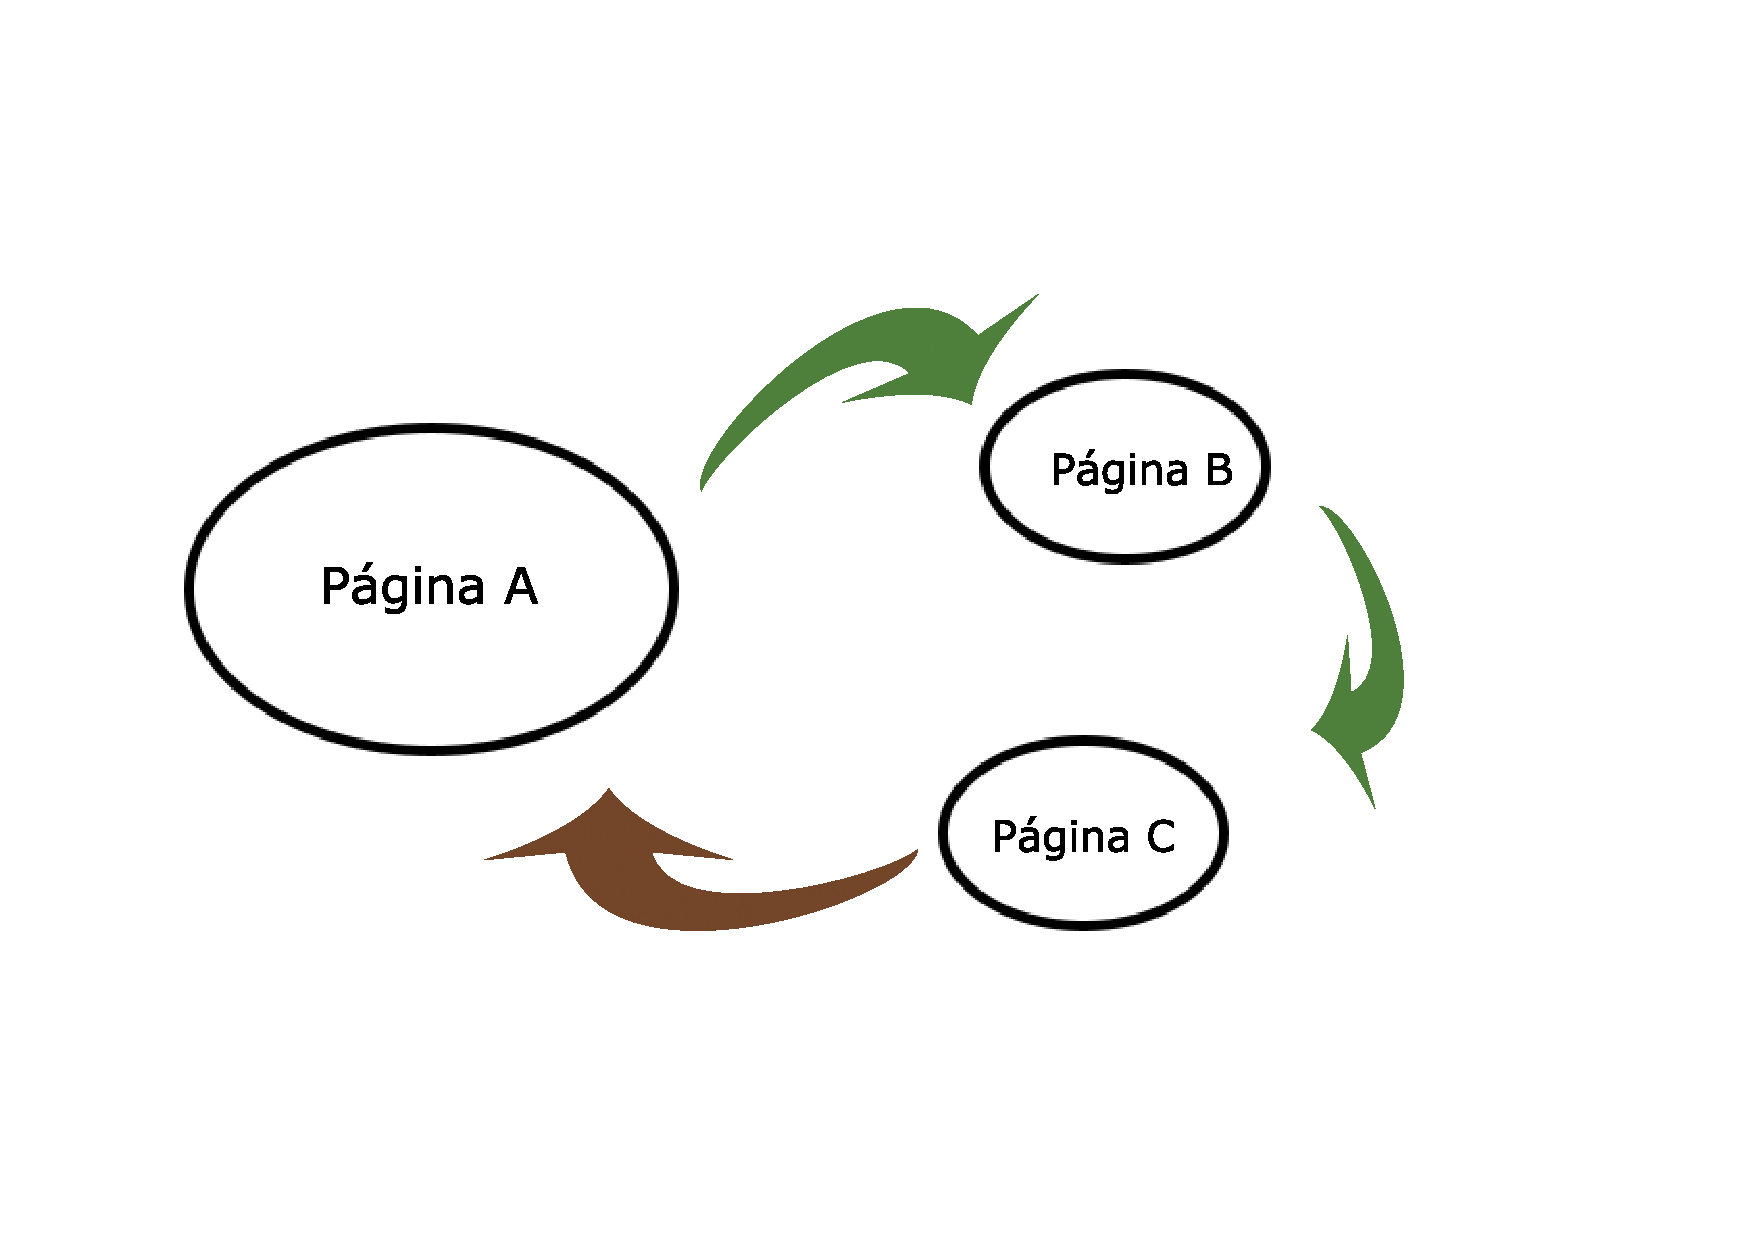
\includegraphics[width=2.5in]{loop2.pdf} }}
\caption{Figura (a) exibe o problema ocorrendo já na página seguinte.}
\label{fig6}
\end{figure}

Neste projeto opotou-se pelo uso de uma biblioteca de crawling que permite o seguimento de URL de páginas e extração de informações sem ter que se preocupar em programar explicitamente Request e Download de páginas da Web.

A Biblioteca escolhida foi o Scrapy, na versão 0.24.4, desenvolvida em Python, que possibilita a criação da lógica de URLs a serem seguidas usando regras conhecidas como \textit{Rules}. As \textit{Rules} são classes com parametros que definem se as URLs podem ou não ser inseridas na lista de processamento. Esses parametros recebem expressões regulares que serão usadas na analise das URLs. Nas Rules também é definido se a URL deve ter seu conteúdo HTML processado pelo parse ou se deve ter apenas as informações href das tags $<$a$>$ extraídas.

Como os websites a serem utilizados possuem conteúdo estático sem uso de Ajax, o Scrapy atende as necessidades básicas de download e parseamento dos websites. Se for necessário extrair informações dinamicamente geradas por AJAX pode ser utilizado o Scrapy com extensão para Firefox ou outra biblioteca de crawling que permite o download do código-fonte da página como visualizado pelos browser, como a biblioteca Selenium.

Scrapy, assim como Python, está disponível para Windows e Linux. Nesse projeto foi utilizado a versão para Windows de 64bits.

\subsubsection{Links Duplicados}

Para se evitar o problema de loops durante o crawling, URLs já processadas precisam ser ignoradas durante a extração de URLs de novas páginas.

Adicionar uma URL já processada a uma lista usada para verificação de URLs já visitadas evita esse problema, porém há casos em que duas URLs com a mesma quantidade de parametros, mas que possuem ordenações diferentes, levam a uma mesma página. A fim de evitar re-processar páginas iguais simplesmente pela ordem dos paramêtros estarem diferentes a biblioteca Scrapy não salva as URLs em si, e sim uma representação das URLs mencionadas como "impressão digital" na documentação do Scrapy. 

Para gerar as "impressões digitais" a biblioteca Scrapy reorganiza os paramêtros de uma URL por ordem alfabética e gera a partir da URL resultante o MD5.


Exemplo de URLs que resultam na mesma impressão digital:


https://www.mangaupdates.com/series.html?page=2\&letter=AF

https://www.mangaupdates.com/series.html?letter=AF\&page=2


\subsubsection{Utilizando Scrapy}

Scrapy é uma biblioteca com todos os recursos necessários para extrair dados de um website, utilizando \textit{Requests} para download do código-fonte de websites e \textit{Parse} para processamento desse código-fonte. Os Requests e Parses são realizados por meio de classes conhecidas como \textit{Spider}.

Um novo projeto Scrapy pode ser iniciado pela linha de comando e ao ser iniciado será criado uma estrutura pronta de pastas e arquivos padrões com algumas configurações pré-determinadas.\newline 

 
\dirtree{%
.1 /.
.2 scrapy.cfg.
.2 projeto\/.
.3 \_\_init\_\_.py.
.3 items.py.
.3 pipelines.py.
.3 settings.py.
.3 spiders\/.
.4 \_\_init\_\_.py.
.4 spider1.py.
.4 spider2.py.
}

Para a visitação de URLs e extração de dados dos websites a biblioteca Scrapy utiliza as classes \textit{Spider} armazenadas na pasta "spiders". Essas classes devem herdar de pelo menos um tipo de spider disponível no Scrapy, cada um com sua implementação única.

A classe que escolhemos herdar para criar nossos spiders é a \textit{CrawlSpider} que implementa o método \emph{parse}, método esse que utiliza as regras definidas para ou seguir uma URL ou efetuar processamento do código-fonte da URL. Quando definimos as regras, em um objeto iterável com nome "rules" na classe, indicamos por meio de expressão regular as páginas que podem ser seguidas e as páginas que devem ter seu conteúdo extraído, parseado e enviado para um método callback. Pode apenas haver um método callback para extração de dados nos spiders que herdam \textit{CrawlSpider}.

Nossa classe \emph{spider} para ser corretamente executada pela biblioteca Scrapy deve informar a propriedade nome do "spider", domínios permitidos para extração de dados sem o schema "http", as URLs iniciais e as regras de visitação e extração de URL.

Ao criarmos o método callback podemos usá-lo de pelo menos dois modos: 

\begin{enumerate}
\item Usá-lo para armazenar as informações extraídas em objetos conhecidos como \textit{items} para serem depois interpretados por diversos métodos \textit{Pipeline} que verificarão se os \textit{items} estão dentro de uma qualificação lógica adequada para serem salvos em Banco de Dados ou salvos em arquivos Json (Esse é o método recomendado pelo Scrapy).
\item Usá-lo diretamente para salvar as informações sem a necessidade de criação de objetos \textit{items}.
\end{enumerate}

Adotamos esse último método na qual as URLs extraídas e parseadas possuem seus dados normalizados para serem salvos no banco de dados no próprio método \textit{callback}.
  
%- alguma intenção original foi abandonada? alguma foi adicionada?
 
 
 
\subsubsection{Implementando acesso ao Banco de Dados}

Para acesso ao banco de dados PostgreSQL, em Python, foi utilizado a biblioteca Psycopg2. A biblioteca oferece métodos para conexão com o banco de dados, para execução de código SQL e para controle de transações.

A partir desses métodos básicos criamos uma classe de conexão ao banco de dados, com métodos para inserção e para atualização de dados que manipulem as informações nas tabelas mantendo a integridade lógica dos dados. 

Embora o Banco de Dados seja responsável por manter a integridade quanto aos tipos de dados a serem inseridos e existência de chaves-primárias e estrangeiras, ele não verifica se a associação realizada é a pretendida. Por exemplo, se queremos associar o autor A ao Livro A e associamos por algum equivoco o autor B, isso é considerado uma falha na integridade lógica dos dados. 

\subsubsection{Tratamento de Erros e Transactions}

Algumas das páginas processadas pelo \textit{parse} podem ter variações na formatação HTML, que podem originar erros na integridade lógica do Banco de Dados. Assim usando o conceito de exceções, quando ocorre uma falha na inserção de algum conteúdo da página processada pelo \textit{parse} todas as operações executadas com os dados da página são descartadas, usando \textit{Rollback} quando uma Exception ocorre, e a URL da página e informações sobre o erro são inseridas em um arquivo de \textit{Log} para analise posterior.

Somente após realização com sucesso, de todas as operações, é finalmente efetuado \textit{Commit} na transação. Permitindo assim que apenas dados formatados e relacionados corretamente sejam salvos no Banco de Dados.

\subsubsection{Itens Relacionados}

Alguns dos websites escolhidos a terem seu conteúdo extraído nas páginas de detalhes de seus itens também fornecem informação de itens relacionados, listando esses itens em tags $<$a$>$. Esses itens podem ser livros, mangás ou figuras de ação. Cada página fornece informações que ajudam a determinar o tipo de item e em qual tabela será salvo.

Esses relacionamentos entre itens também são salvos no banco de dados desse projeto. Atráves das tags $<$a$>$ podemos extrair a URL do item e consultando a tabela spider\_item do banco de dados podemos identificar se o item já foi salvo, precisando portanto apenas inserir o relacionamento nas tabelas adequadas. Se um item ainda não foi criado, um item com valores nulos é inserido no banco de dados, na tabela apropriada, a fim de se obter um id e seu id e sua URL são adicionados na tabela spider\_item.

A tabela spider\_item é consultada sempre que uma página é processada para ter suas informações extraídas e salvas no banco de dados. Se a página que estiver sendo processada foi localizada na tabela spider\_item o item é atualizado utilizando o id registrado ao invés de ser criado um novo item. Assim é mantido o relacionamento mesmo entre itens que ainda não tiveram suas URLs processadas pelo crawler.

\subsubsection{Definindo Franquias}

Para alcançarmos o objetivo de fazer uma visualização de dados com extração de informações relacionadas a franquias, precisávamos identificá-las e criá-las a partir do conteúdo salvo no Banco de Dados. 

Escolhemos criar as franquias na execução do próprio Crawler, utilizando o nome dos itens e quando disponível os nomes dos itens relacionados.

Para a criação do nome das franquias é identificado o nome principal nos títulos dos itens, para isso removemos subtítulos, que podem ser identificados como parte posterior de um hífen ou parte dentro de parenteses, dos títulos. Com o nome principal podemos pesquisar por franquias na tabela collection que possuem o mesmo nome, ou criar uma nova se nenhuma franquia for localizada.

No título de um item abaixo temos um exemplo de título a esquerda e subtítulo a direita:

Kidou Senshi Gundam Unicorn - Char second comming

Se um item possui algum item relacionado salvo no banco de dados, antes de criamos uma nova franquia caso nossa busca não retorne resultados é executado uma busca recursiva, utilizando o recurso WITH RECURSIVE do PostgreSQL, a fim de retornar o nome e franquia de todos os itens relacionados ao atual. Se uma franquia associada a um item é encontrada os demais itens ainda não associados a franquia são atualizados.

Se nenhuma franquia associada é encontrada será necessário criá-la. Se existem itens relacionados, o nome da franquia será criado usando os nomes em sequência mais comuns entre os nomes principais dos itens. Se não existem itens relacionados será utilizado apenas o nome principal do item atual na criação da franquia.

Nos títulos abaixo podemos identificar o nome mais comum entre os nomes principais, neste caso Fairy Tail:
 
Fairy Tail - Season 1

Fairy Tail Freezing - Season 1 


Com esse método há possibilidade de associar a franquias itens com nomes semelhantes ou iguais que pertencem a franquias distintas. Como exemplo, existe o mangá Magician criado por Sarae Kim e existe também o mangá homônimo criado por Yuriko Matsukawa que possuem histórias diferentes e que não se passam no mesmo universo fictício. Para corrigir casos assim é necessária uma verificação manual da associação de franquias posterior a execução do crawler.

\subsubsection{Determinando Idioma}

Alguns dos website escolhidos além de fornecerem o título de itens em inglês também fornecem os títulos em outros idiomas como em japonês, em francês ou em português. Para que esses títulos fossem salvos no banco de dados foi necessário determinar o idioma a qual pertencem. 

A biblioteca Langid, para Python, consegue sem a necessidade de treino prévio identificar até 97 idiomas. Langid oferece o método \emph{classify} para identificar o idioma, que retorna o idioma e a probabilidade desse idioma estar correto em determinado texto. Embora a probabilidade de acerto quando se utiliza frases curtas esteja abaixo de 50\%, para idiomas com caracteres distintos como o japonês ou coreano essa probabilidade aumenta e pode chegar até 99\%.

Portanto determinamos um valor mínimo para utilizar o idioma detectado pelo Langid. Quando a probabilidade retornada ultrapassava o valor de 70\% usavamos o idioma identificado, mas quando esse valor não era alcançado utilizavamos o idioma padrão  determinado. O idioma padrão para muitos itens foi determinado a partir do país de origem.

\subsection{Visualização de Dados}

Para visualização de dados extraímos do banco de dados textos e representamos a variação na quantidade entre os textos, exibindo-as como uma nuvem de bolhas ou uma nuvem de palavras. 
Usamos a estrutura de dados Tabela de Área Somada, também conhecida em Visão Computacional como Imagem Integral, para identificação de espaços ocupados e realizamos uma distribuição aleatória na imagem de nossos objetos: as bolhas ou as palavras.
Para esse fim utilizamos a biblioteca Numpy para manipulação de vetores multidimensionais, gerando assim a Tabela de Área Somada, e a biblioteca PIL para desenhar palavras, desenhar formas e salvar a imagem resultante.


A imagem abaixo ilustra a sequência adotada para criação de nossas nuvens. Essas etapas serão melhor explicadas nos próximos tópicos.

\begin{figure}[H]
\centering
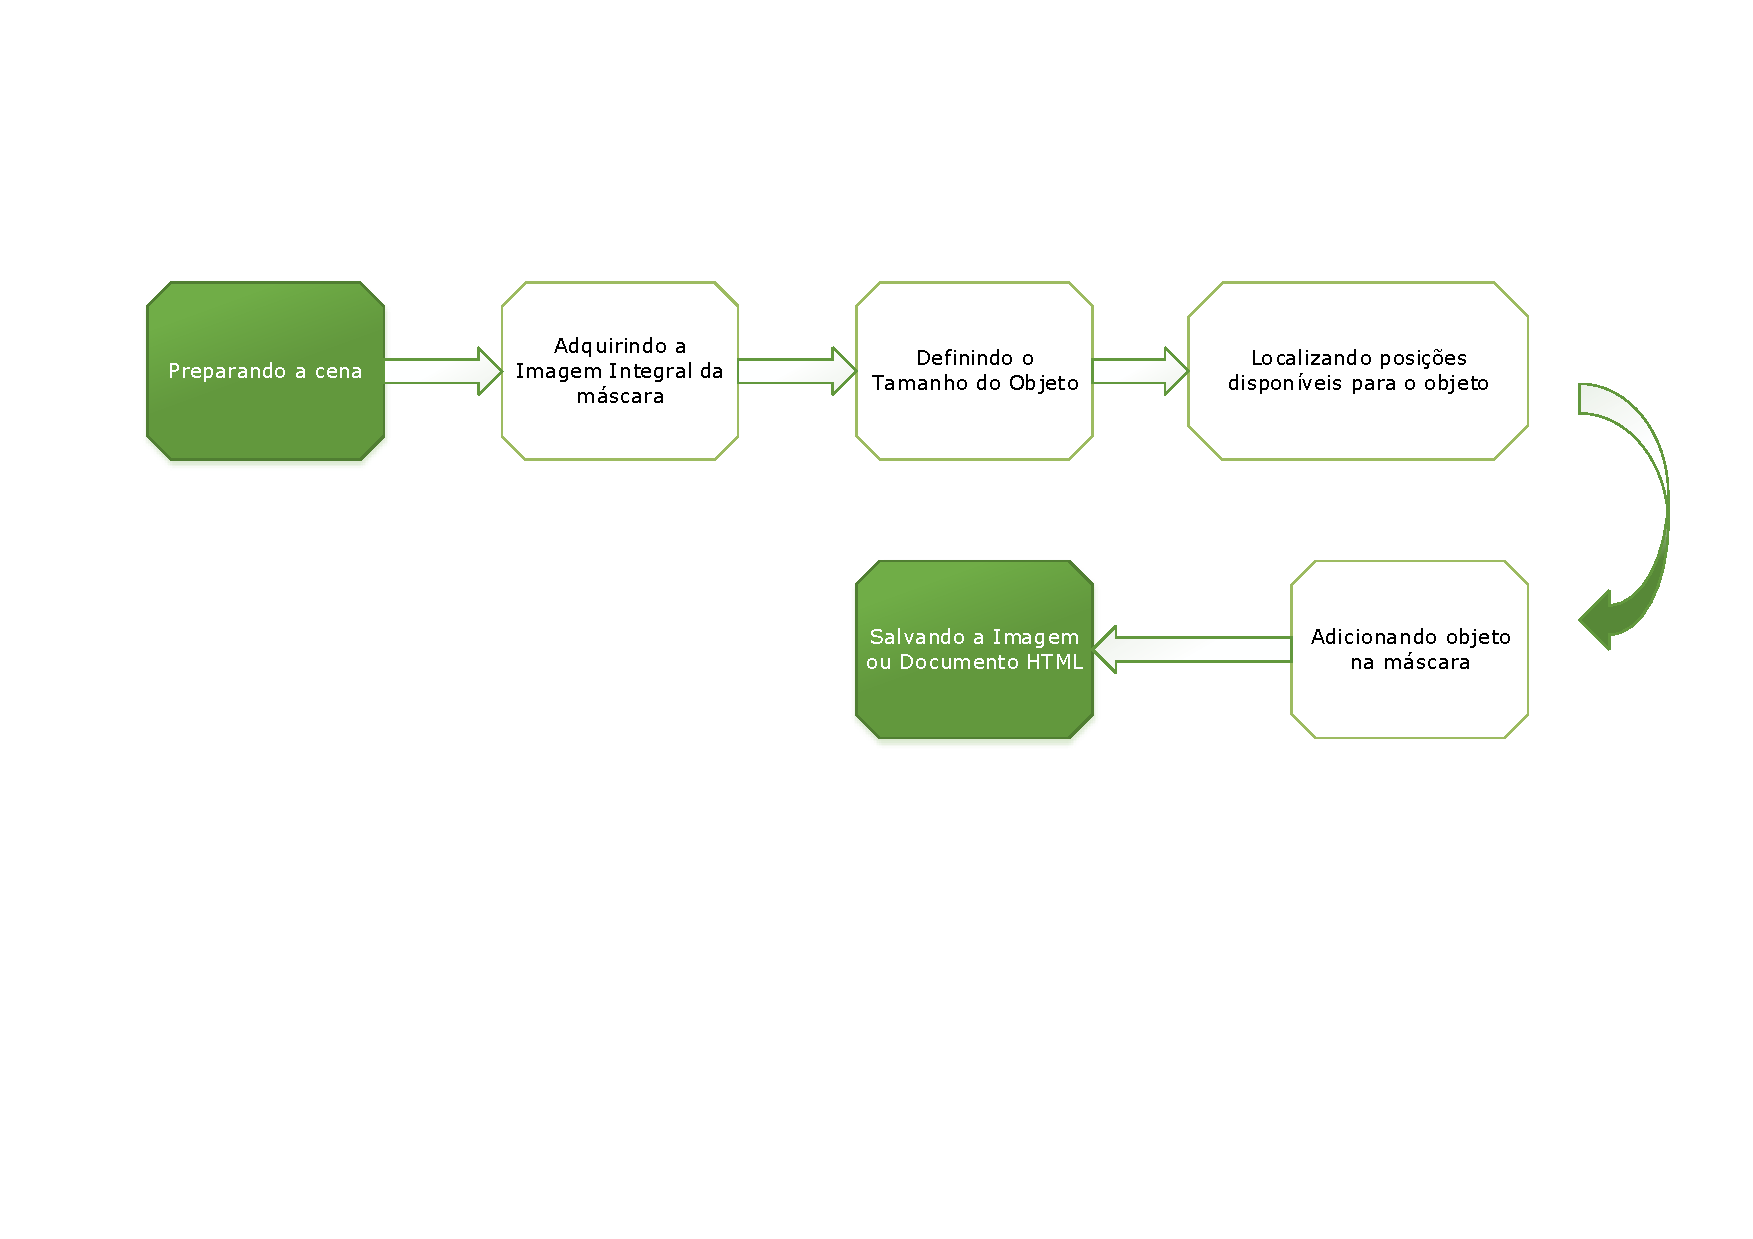
\includegraphics[width=1\textwidth]{fluxo.pdf}
\caption{Etapas 2 a 4 são executadas múltiplas vezes enquanto ainda existir objetos a serem posicionados.}\label{company}
\end{figure}


\subsubsection{Preparando a Cena}

Utilizando a biblioteca de processamento de imagem preparamos um fundo com tamanho determinado que usaremos para posicionar nossos objetos. 
Qualquer seguimento da Tabela de Área Somada com valor diferente de zero é considerado ocupado, assim podemos criar uma imagem com fundo totalmente preto, utilizando toda a área disponível, ou podemos criar uma área limitada com ilustrações ou textos resultando em uma máscara para nossa visualização.
A cor preta é representada pelo valor 0 e ao converter a imagem preparada em um vetor multidimensional com Numpy podemos obter a matriz inicial que será utilizada para gerar a Tabela de Área Somada inicial.

\begin{figure}[H]
\centering

\includegraphics[width=0.8\textwidth]{e-comp-2450.pdf}
\caption{Imagem utilizada como máscara} \label{collaborator}
\end{figure}


Para uso da Tabela de Área Somada é utilizado como máscara imagens na escala cinza, assim podemos trabalhar apenas com um valor variante para cada pixel da imagem.

\subsubsection{Obtendo a Tabela de Área Somada}

A Imagem Integral é uma matriz obtida a partir de uma imagem que possui um único canal de cor. Cada valor na Tabela de Área Somada representa o produto resultante da soma de todos os valores anteriores da imagem.

Utilizando uma matriz inicial criamos a Tabela de Área Somada usando cumsum do Numpy. As dimensões da matriz inicial e a Tabela de Área Somada são as mesmas, o que as diferenciam são os valores de cada linha e coluna da matriz.

\begin{figure}[H]
\centering
\mbox{\subfigure{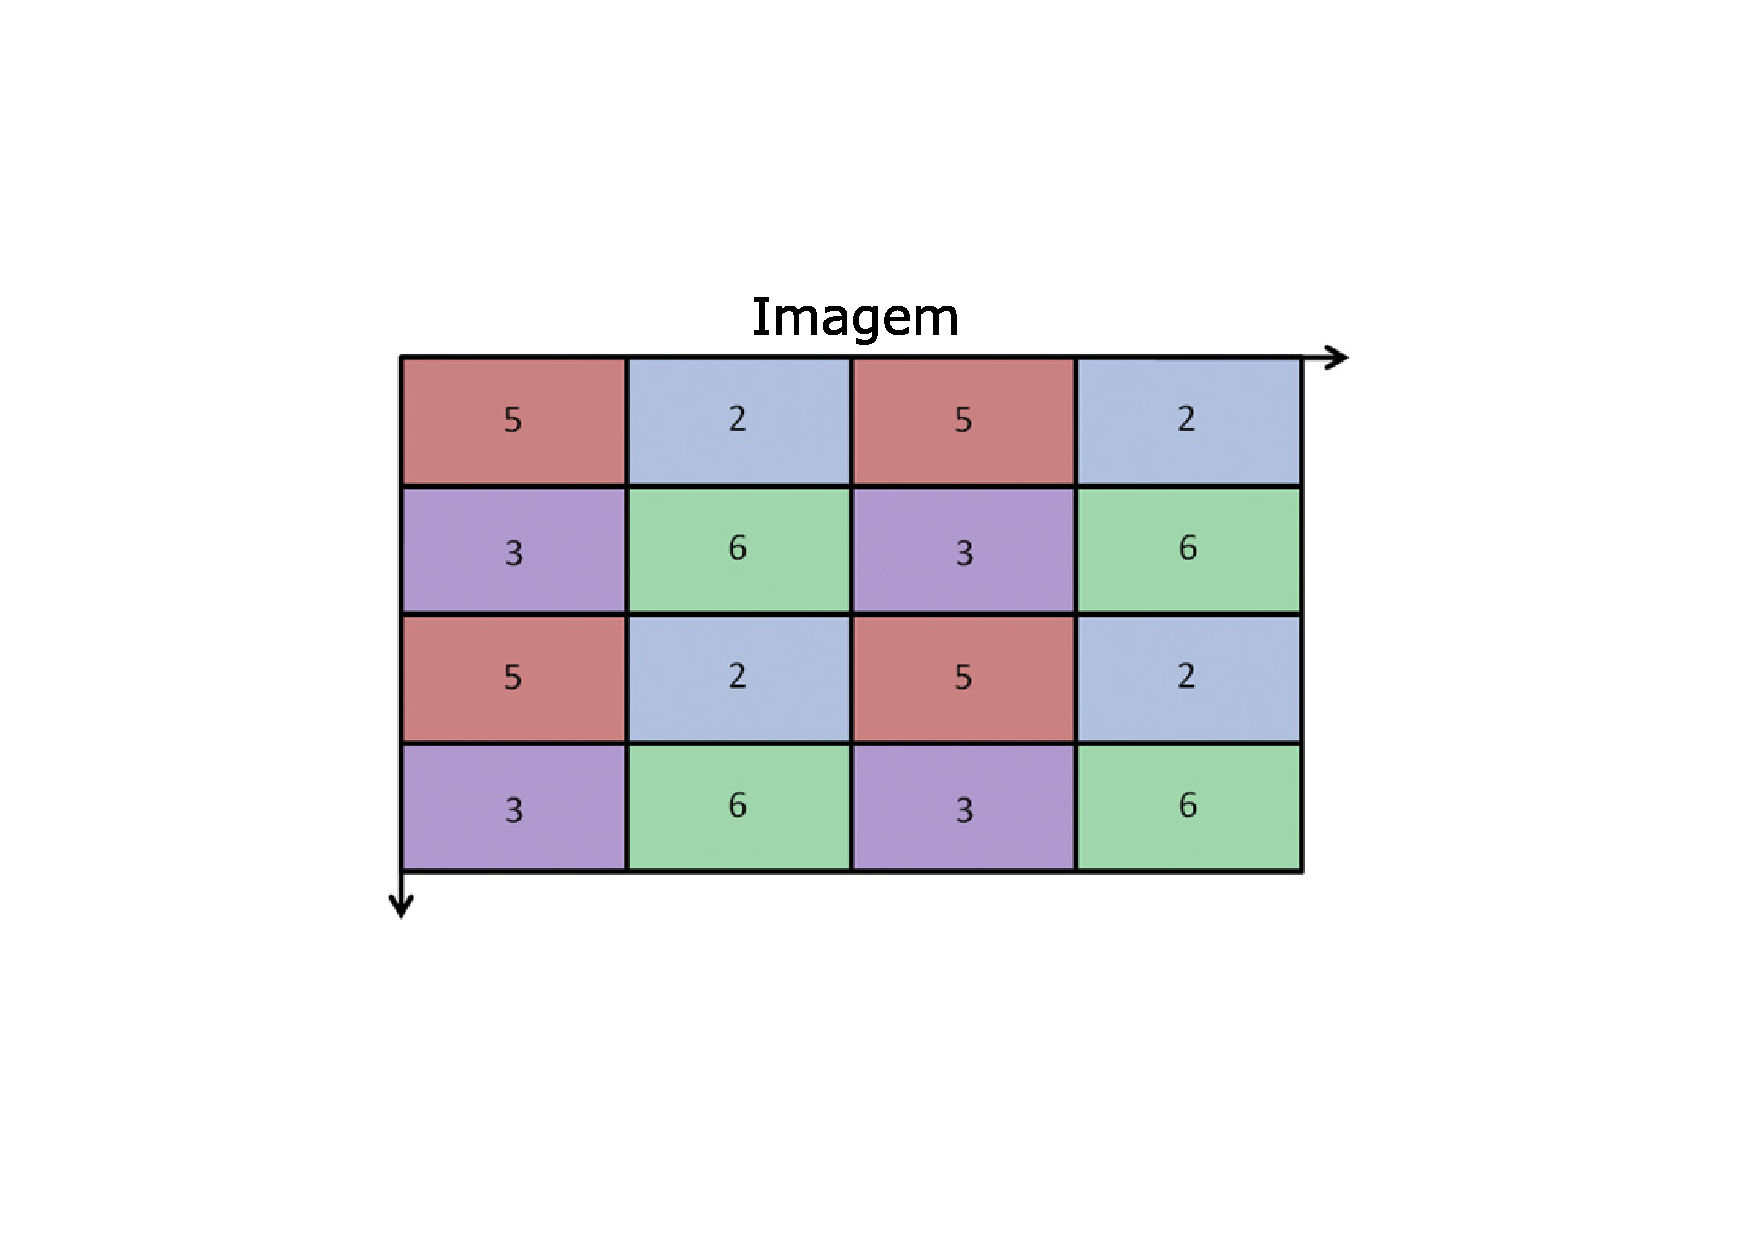
\includegraphics[width=3in]{image.pdf}}\quad
\subfigure{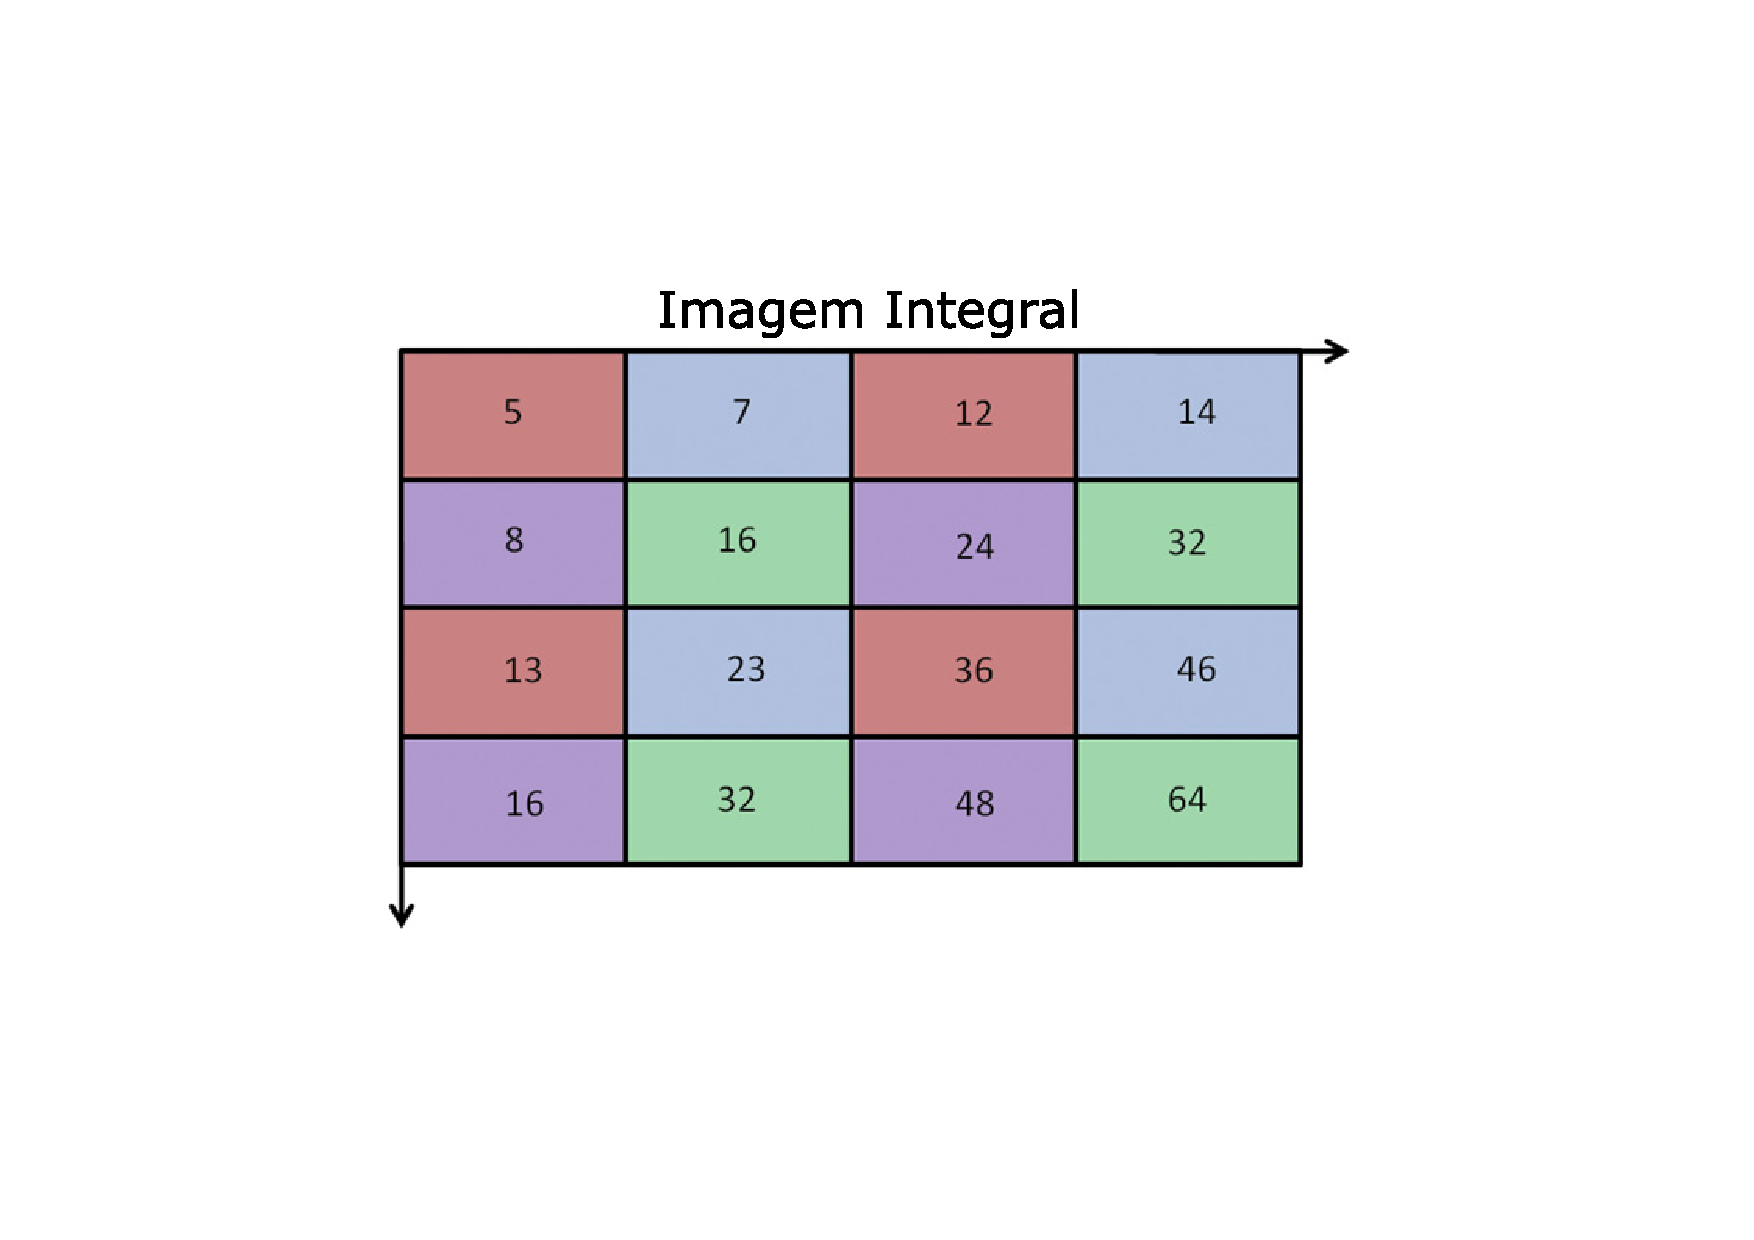
\includegraphics[width=3in]{integral.pdf} }}
\caption{Figura (a) representa a matriz formada por uma imagem com apenas um canal de cor. Figura (b) representa a Imagem Integral obtida a partir dos valores da figura (a).}
\label{fig6}
\end{figure}

\subsubsection{Definindo o Tamanho dos Objetos}

Ao obtermos nossos objetos, palavras e círculos, do Banco de Dados também selecionamos informação numérica que representam um ranking entre os objetos. Alguns dos valores numéricos utilizados como ranking são: quantidade de itens da franquia, valor em reais para adquirir todos os item da franquia, volume mínimo em $m^3$ necessário para armazenar todos os itens da franquia.

Para definir o tamanho dos objetos e manter uma proporção ao alor do ranking, usamos a razão do valor do ranking pelo logaritmo natural desse valor.

Como nossos resultados possuiam um ranking na casa dos milhares, dividimos por 10 o resultado obtido para que não sejam gerados tamanhos demasiadamente grandes. 

\begin{equation} 
tamanho = \frac{c * ranking}{\ln(ranking + 10)}
\end{equation}

Para evitar divisão por zero é somado o valor 10 ao número do rankeamento antes do cálculo do Logaritmo Natural.

Onde:

\begin{itemize}  
  \item $c -\; raz\tilde{a}o\,entre\,a\, \acute{a}rea\,da\,cena\,e\,a\,quantidade\,
  de\,objetos$
  \item $ranking -\; valor\,inteiro\,que\,representa\,o\,valor\,do\,objeto\,em\,relaç\tilde{a}o\,aos\,outros$
\end{itemize}

Para colocar os textos dentro dos círculos foi necessário determinar o tamanho que a fonte do texto deve possuir para não ultrapassar o diâmetro. Para isso foi utilizado o seguinte cálculo:

\begin{equation} 
tamanho = \frac{d * 1.5}{c}
\end{equation}

Onde:

\begin{itemize}  
  \item $d -\; di\hat{a}metro\,do\,c\acute{i}rculo$
  \item $c -\; quantidade\,de\,caracteres\,no\,texto$
\end{itemize}


\subsubsection{Determinando a posição dos Objetos}

Para verificarmos se um espaço está disponível na cena para nossos objetos precisávamos verificar se já não existe outro objeto já posicionado no local. 

Conseguimos verificar se o espaço está ocupado ou não calculando o valor na área que nosso objeto ocupa. Se o local em que pretendemos colocar nosso objeto estiver ocupado o resultado do cálculo da área será acima de zero.

Com o cálculo da área saberemos exatamente quanto espaço está sendo ocupado em determinada área e posição. E utilizando a Tabela de Área Somada conseguimos realizar o cálculo da área, em analise assintótica: em tempo constante O(1).

$\acute{a}rea = I(x,y) + I(x + i,y + j) - I(x + i,y) - I(x,y + j).$

Onde:

\begin{itemize}  
  \item $I -\; representa\,a\,matriz\,da\,Tabela\,de\,\acute{A}rea\,Somada$
  \item $i -\; representa\,o\,comprimento\,do\,objeto$
  \item $j -\; representa\,a\,altura\,do\,objeto$
\end{itemize}
 

Ao calcular a área de todos pixels da imagem, que serve de máscara, e adicionar em um vetor os valores que representam a linha e coluna da posição livre, poderíamos escolher randomicamente uma posição livre para adicionarmos nosso objeto.

Com uma posição escolhida informações do objeto, como tamanho e posição, são adicionados a um vetor utilizado posteriormente para geração da imagem final ou exportação para HTML. 

Depois da escolha da posição e inserção do objeto na imagem máscara, a imagem é salva e é gerada uma nova Tabela de Área Somada a partir dessa nova imagem, para uso da verificação de espaço disponível da próxima palavra. 

Quando um espaço disponível não for encontrado o objeto sofre redução de 1 pixel no seu tamanho e novamente é procurado por um espaço disponível.

\subsubsection{Gerando a Imagem Final ou Exportando para HTML}

Com a determinação do posicionamento dos objetos na cena, tamanhos e fontes de texto utilizadas além de gerar uma imagem final também podemos exportar nossa nuvem para HTML utilizando CSS para desenhar e posicionar nossos objetos dentro de uma tag $<$div$>$.

Para gerar a imagem final com nossos objetos posicionados utilizamos os métodos disponíveis na biblioteca PIL para inserção de texto e de elipse e depois salvamos a imagem final em um local determinado. A biblioteca PIL não oferece método para criação de círculo, mas podemos criá-los inserindo uma elipse que terá um raio constante, ou seja uma elipse com dimensões de um quadrado.

Para a crição do HTML consideramos que a posição dos objetos é relativa a uma tag $<$div$>$ com elemento id definida como principal, as mesmas coordenadas [x, y] utilizadas no posicionamento em nossa imagem podem ser aplicadas no posicionamento na tag $<$div$>$ \#principal.

Geramos um documento HTML com nosso CSS adicionado na tag $<$head$>$, que permite uma melhor manipulação posterior de nossos objetos quando o HTML for salvo.

Cada objeto a ser posicionado deve estar dentro de uma tag $<$div$>$ que contêm classes que representam os tamanhos, formas e posições. Essas classes e seus estilos CSS são criados após a determinação de posição de todos os objetos.

Com o posicionamento dos objetos determinado, suas dimensões e outras características definidas, para gerarmos o documento HTML criamos métodos que armazenam em uma variável o texto com o estilo CSS utilizado, para nossos objetos, e em outra variável as tags $<$div$>$ criadas. Ao finalizar o processamento de todas as palavras criamos um novo arquivo com extensão \textit{html} e inserimos o conteúdo das duas variáveis formatadas corretamente nesse novo arquivo. 


\section{Resultados}

Com o uso de crawling foi possível obter uma quantidade considerável de dados. Um resultado mais detalhado pode ser visto a seguir: 

Manga-Updates - Com o crawling do site http://mangaupdates.com foi possível obter 103.774 itens, classificados como Mangás, Light Novels e livros; 34.721 pessoas, que atuam como ilustradores ou escritores; e 1.181 editoras.

My Figure Collection - Com o crawling do site http://myfigurecollection.net foi possível obter 205.041 produtos, incluindo Figuras e 3.440 empresas envolvidas na produção desses produtos.

Anime Characters Database - Com o crawling do site http://animecharactersdatabase.com/ foi possível obter informações de 70.304 personagens e 4.840 dubladores.

Com os resultados obtidos com o crawling foi possível criar 109.274 franquias e associá-las aos itens e aos produtos. Mas, dessas franquias apenas 1.497 possuem mais de um item. Também foi possível relacionar produtos com personagens.

Para obter esses resultados foi necessário a execução do crawler por três dias consecutivos, levando um dia para download e extração das informações de cada site.  

Com as informações armazenadas no Banco de Dados foi possível criar várias visualizações seguindo os dois modelos de visualizações desenvolvidos nesse projeto.

\begin{figure}[H]
\centering
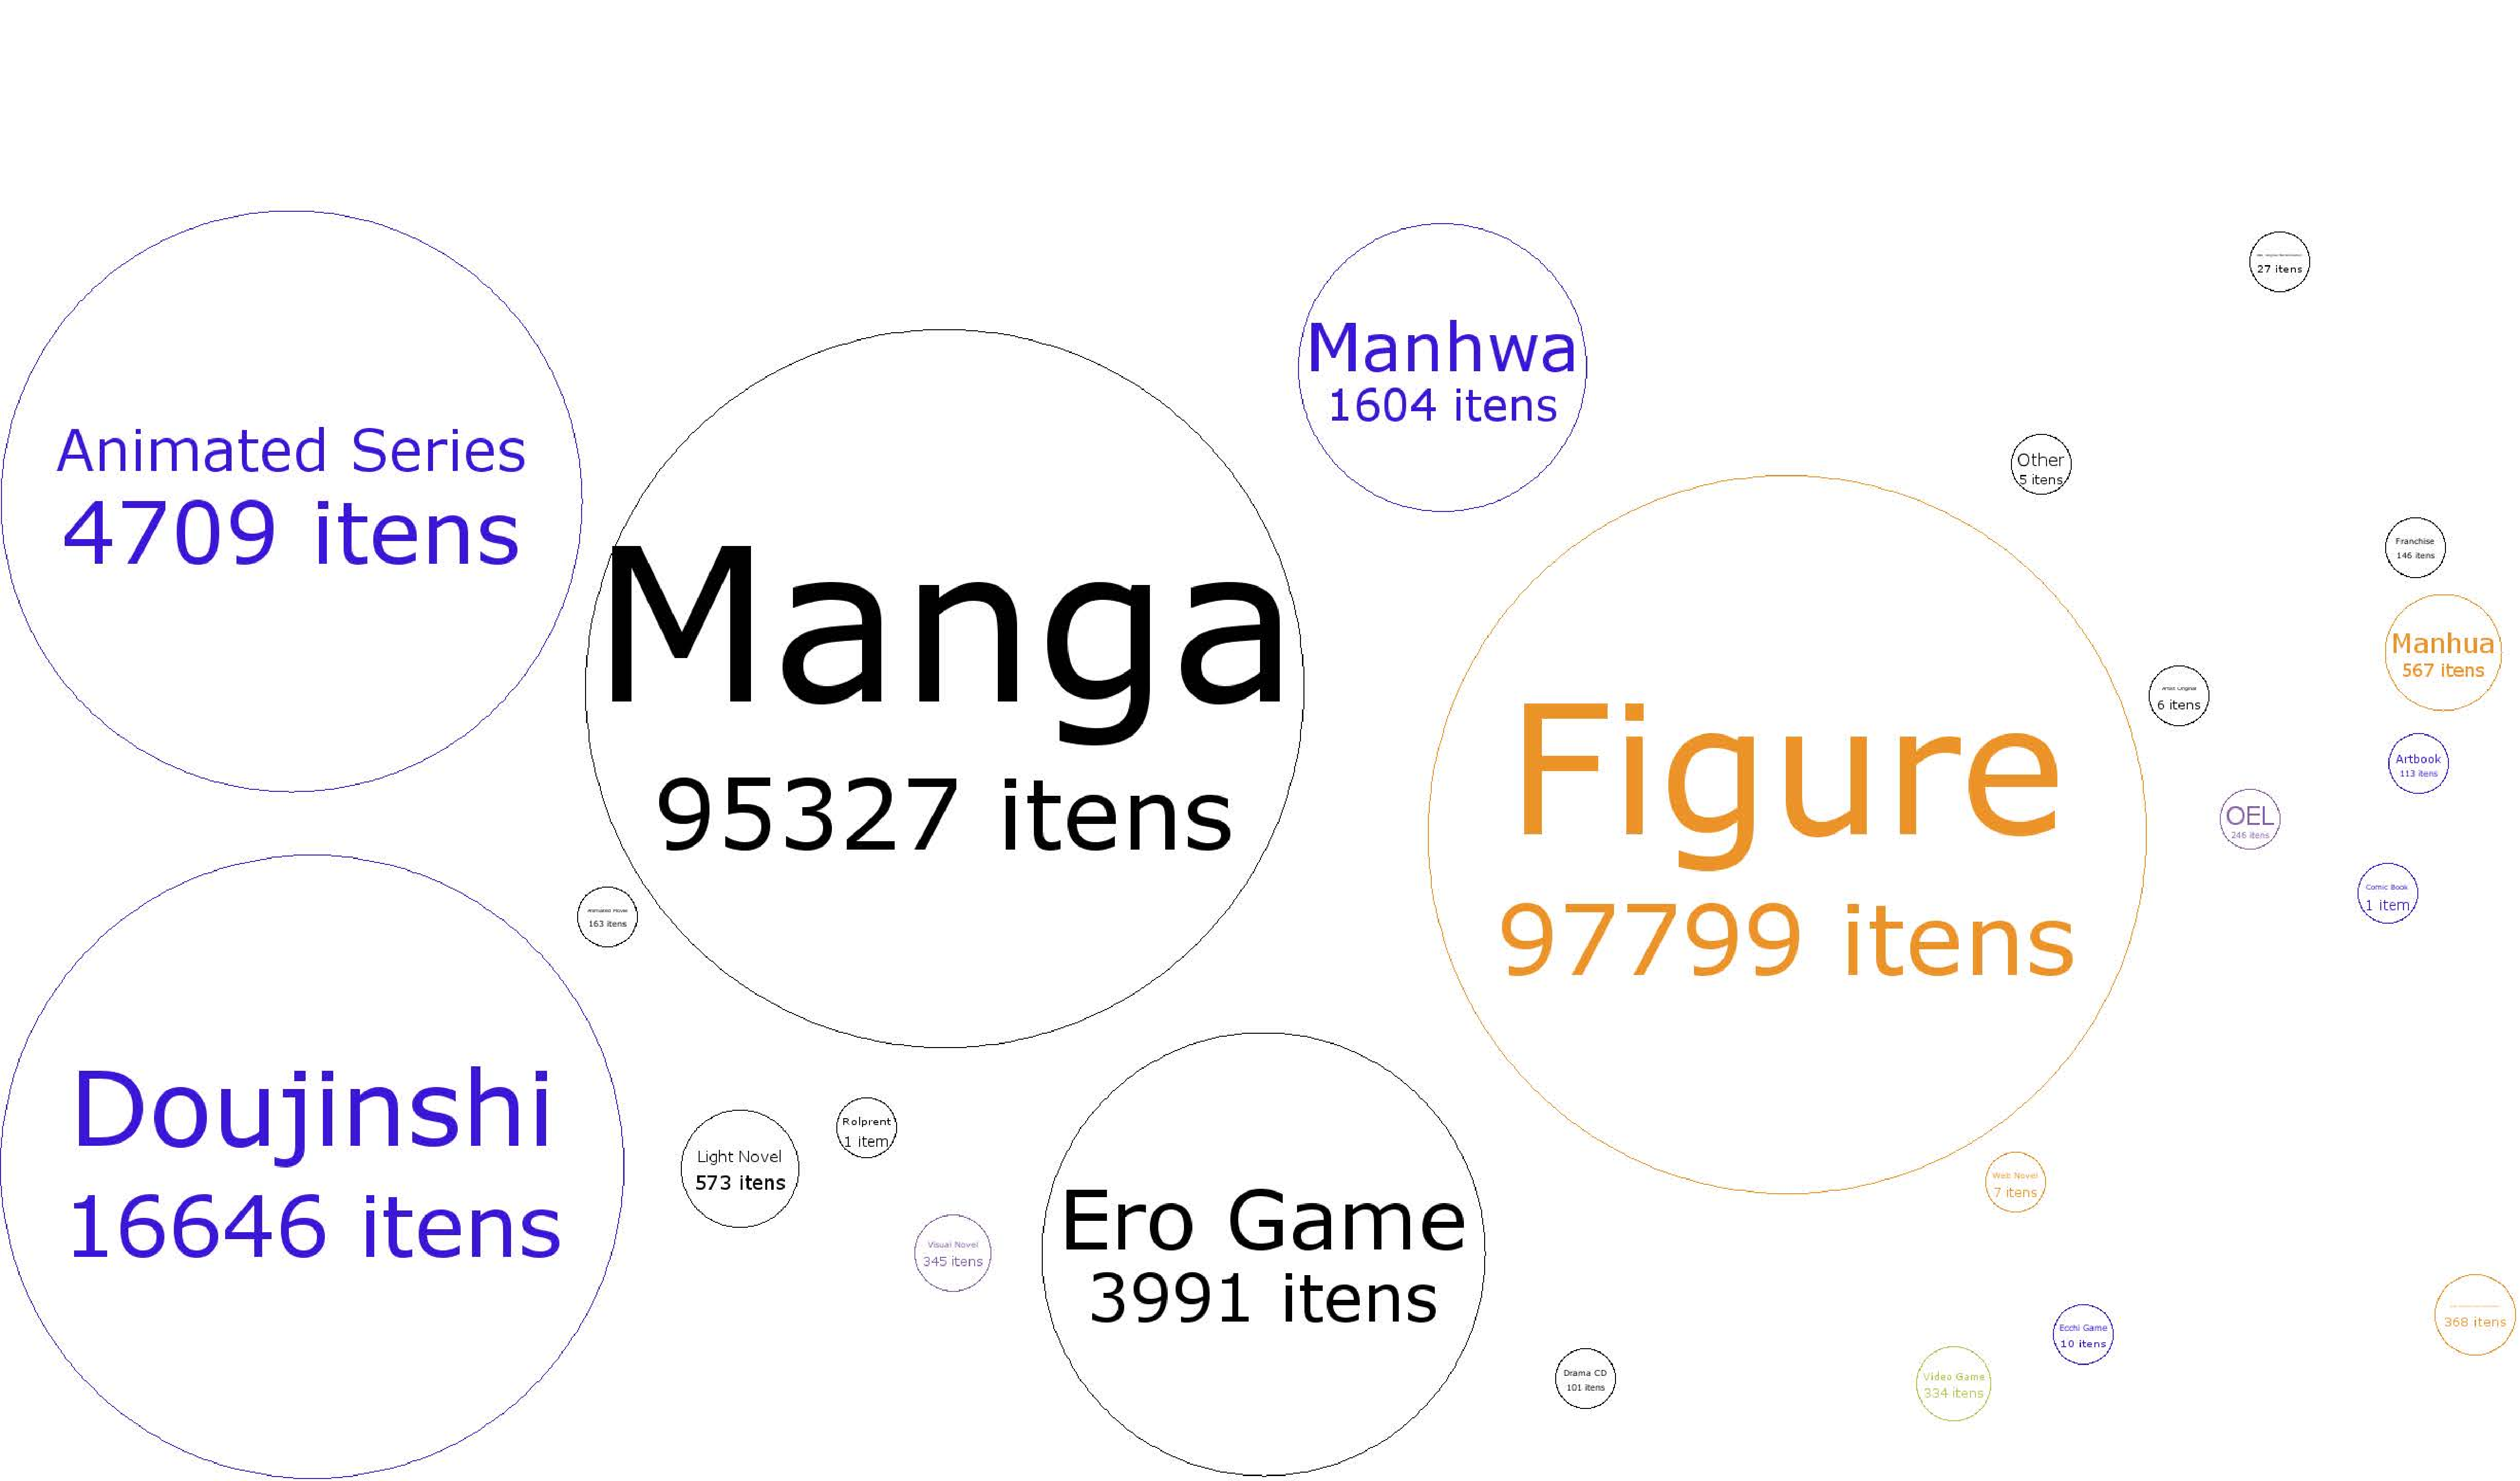
\includegraphics[width=1\textwidth]{item_amount_bubbles.pdf}
\caption{Visualização de dados em nuvem de bolhas. A imagem ilustra a quantidade que cada tipo de item possui. Doujinshi são mangás distribuidos independentemente, geralmente produzidos por artistas iniciantes.} \label{collaborator}
\end{figure}

\begin{figure}[H]
\centering
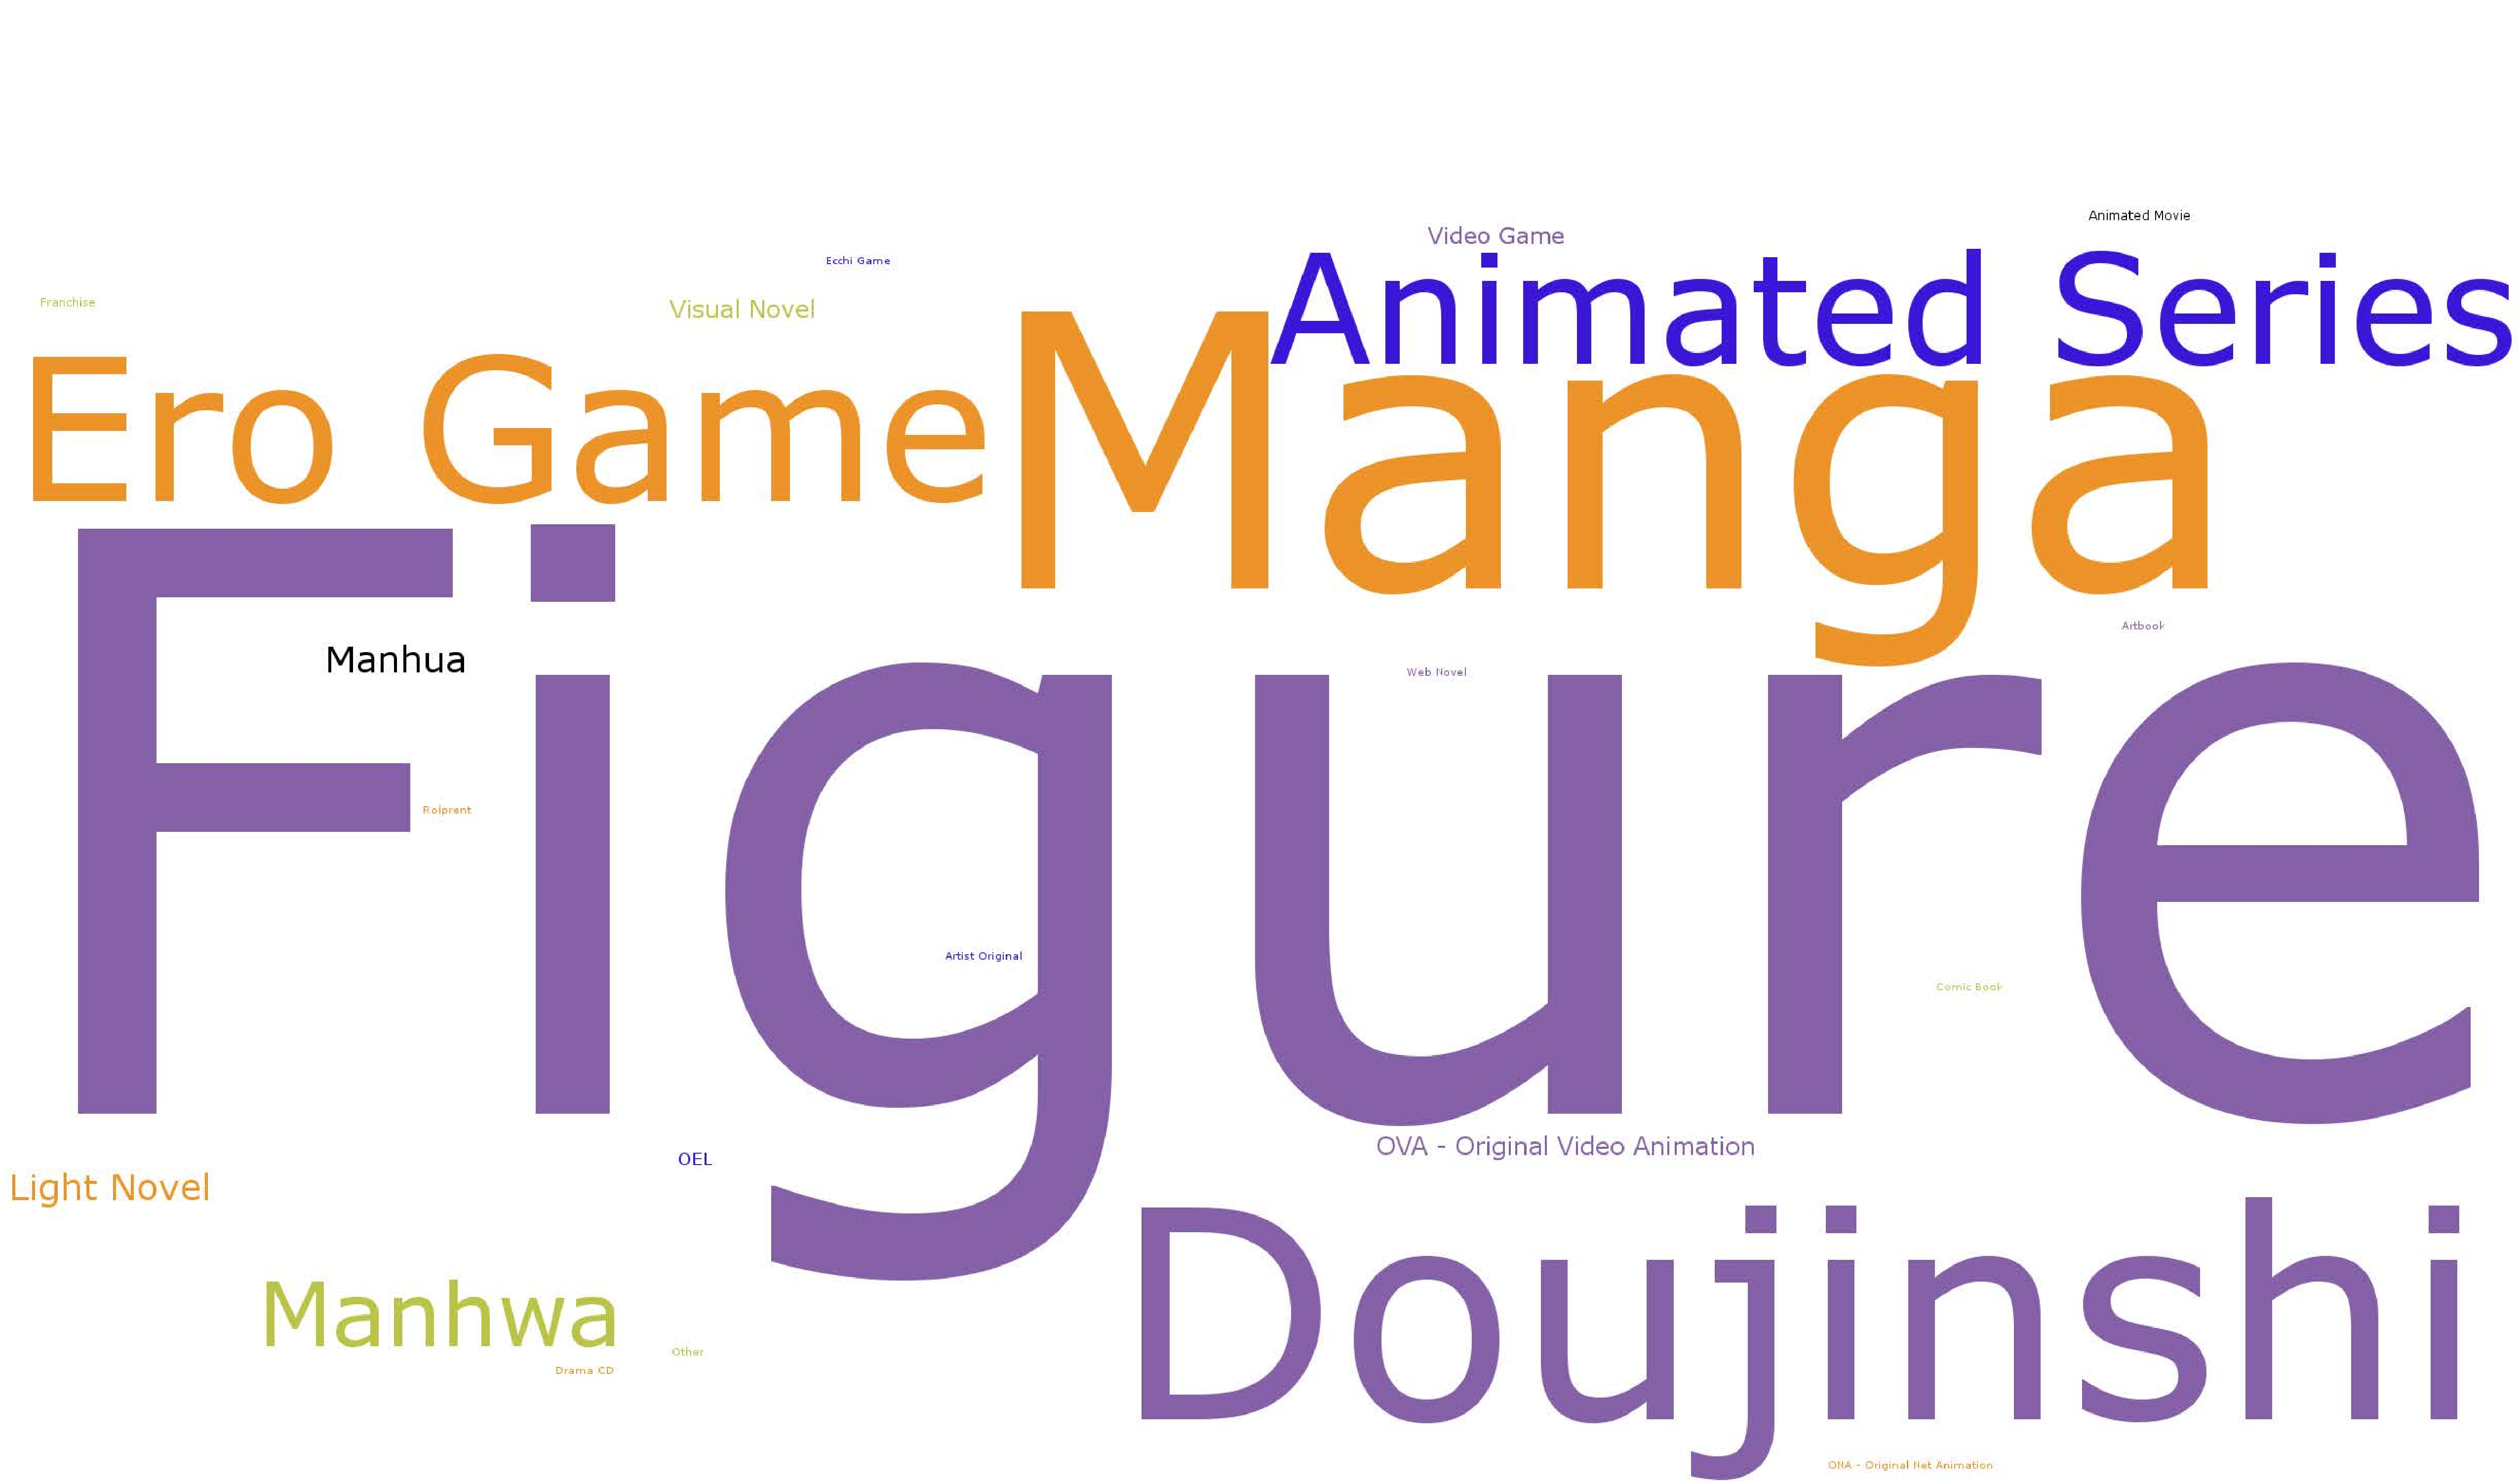
\includegraphics[width=1\textwidth]{items_amount_words.pdf}
\caption{Visualização de dados em nuvem de palavras. A imagem ilustra a quantidade que cada tipo de item possui.} \label{collaborator}
\end{figure}

\begin{figure}[H]
\centering
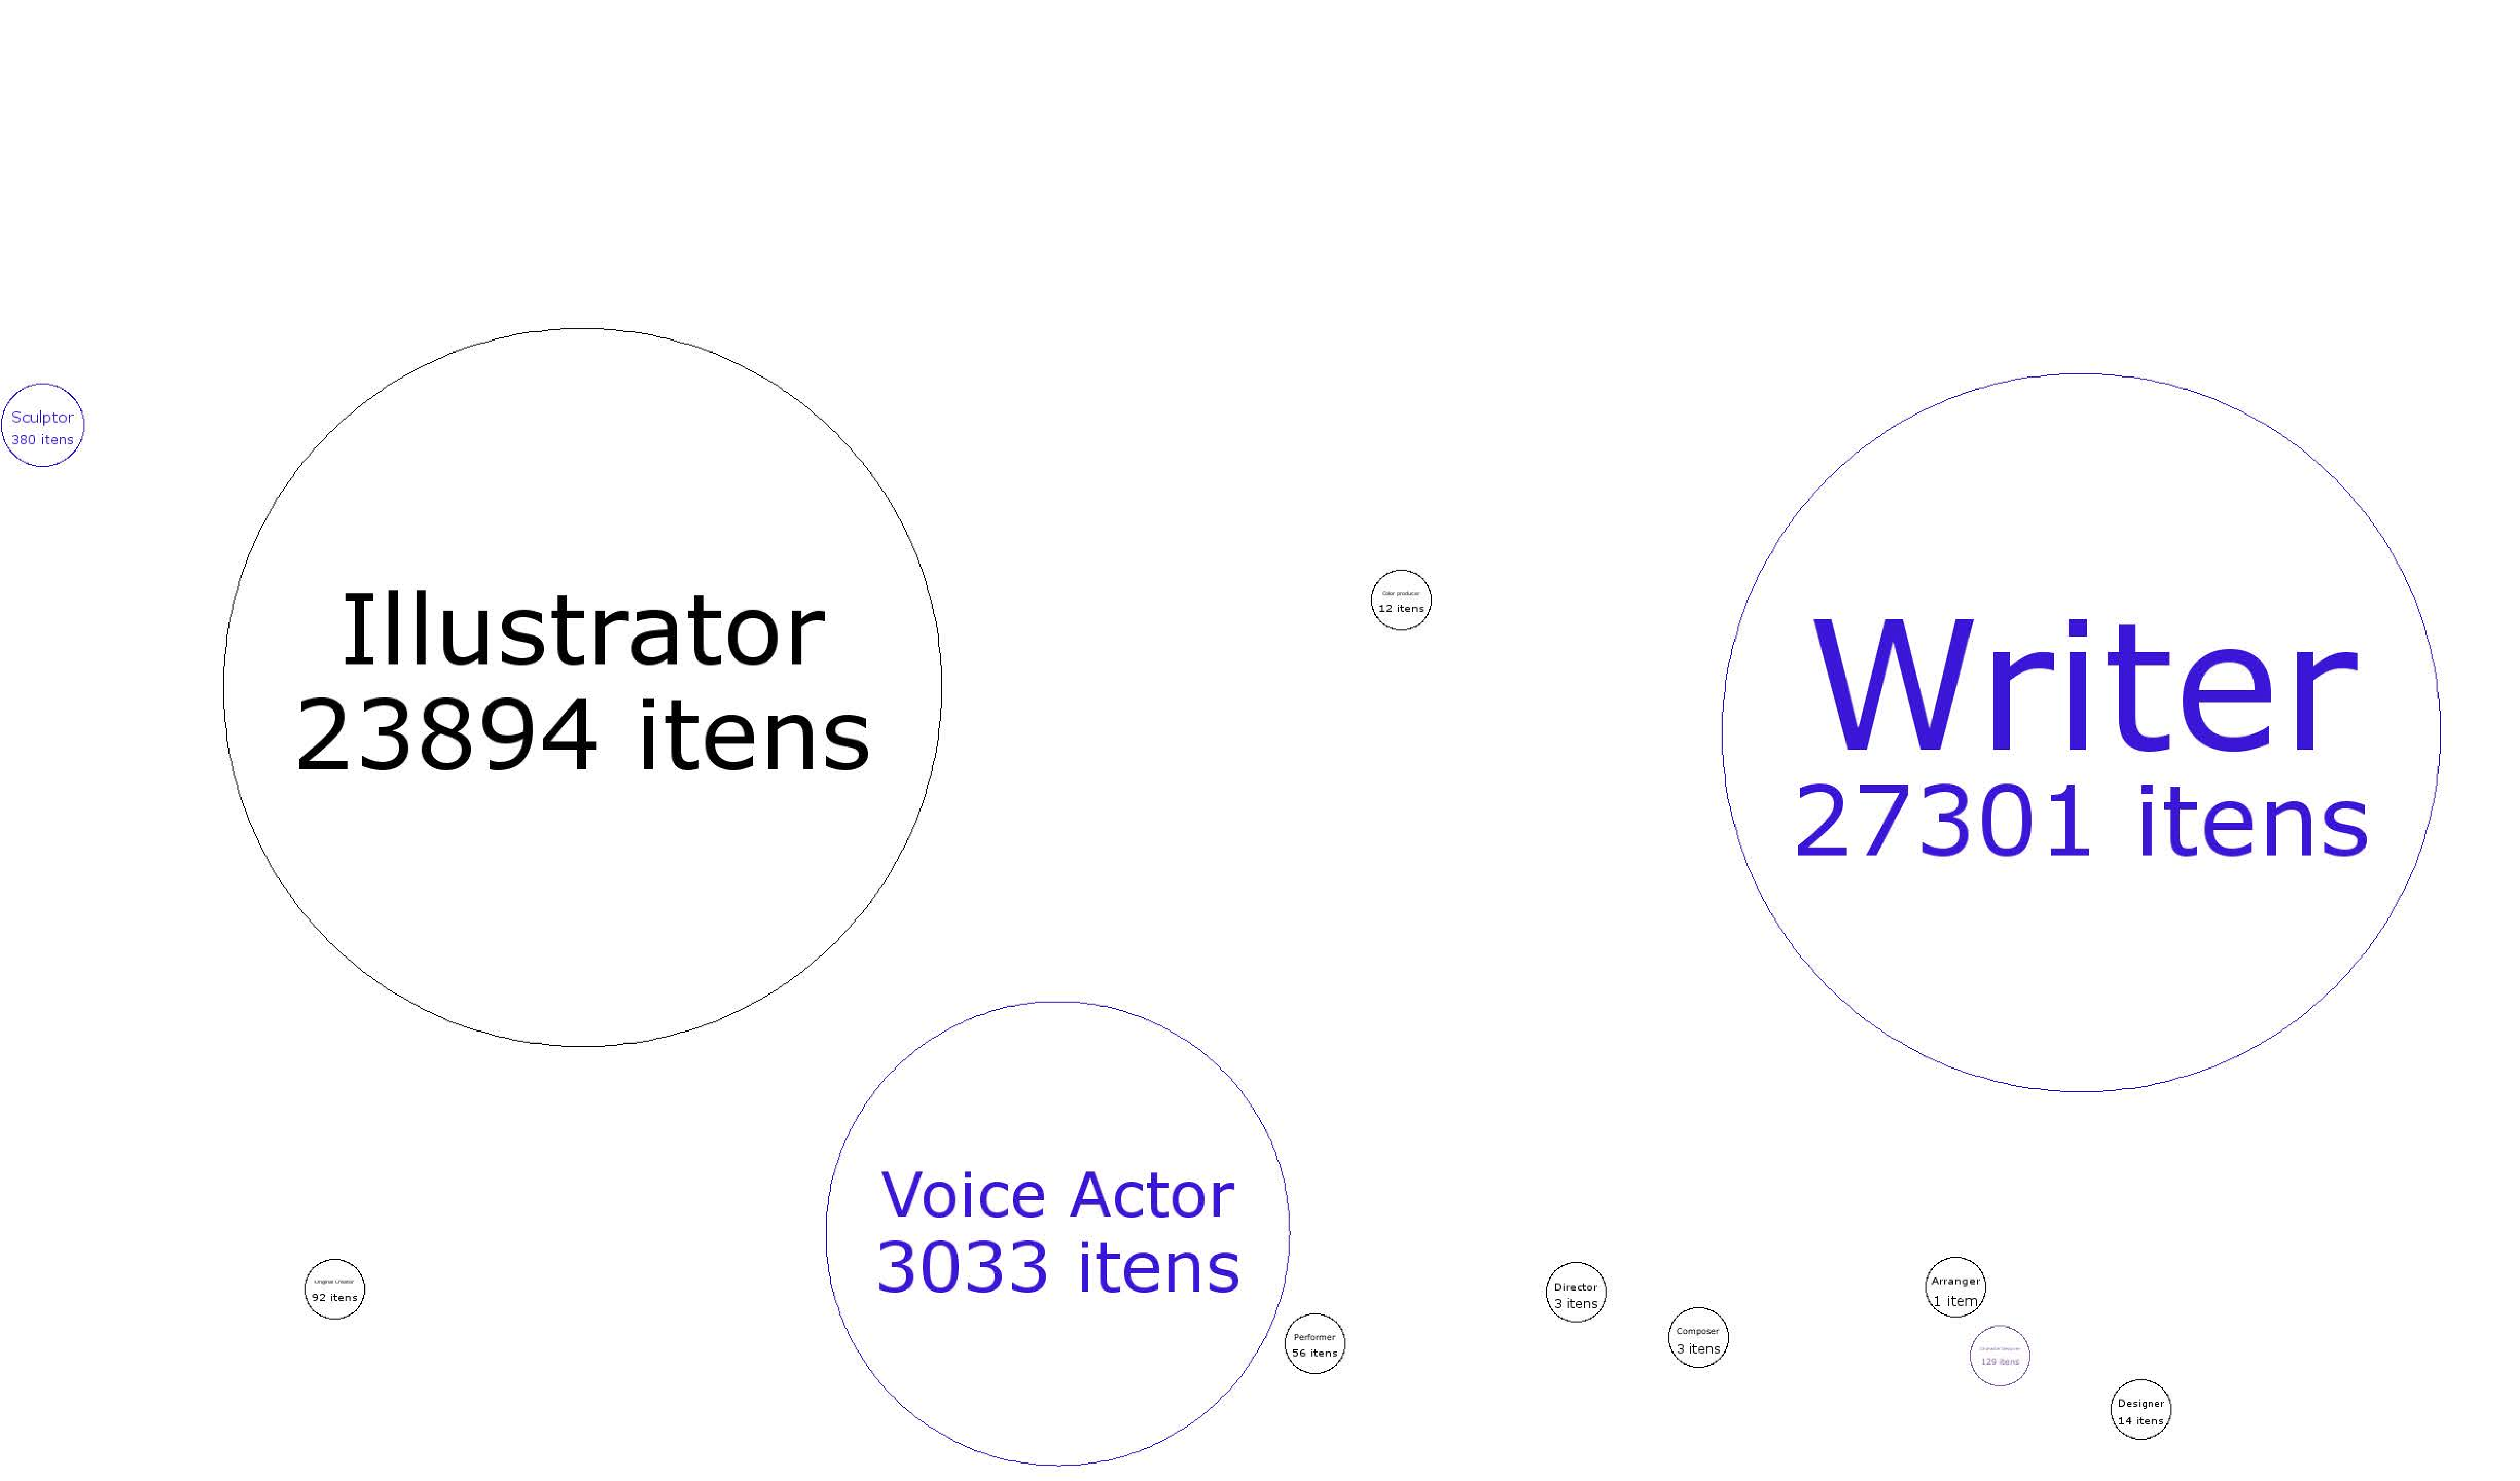
\includegraphics[width=1\textwidth]{people_type_bubble.pdf}
\caption{Visualização de dados em nuvem de bolhas. A imagem ilustra a quantidade de profissionais envolvidos na produção de itens.} \label{collaborator}
\end{figure}

\begin{figure}[H]
\centering

\includegraphics[width=1\textwidth]{people_type-words.pdf}
\caption{Visualização de dados em nuvem de palavras. A imagem ilustra a quantidade de profissionais envolvidos na produção de itens.} \label{collaborator}
\end{figure}

\begin{figure}[H]
\centering
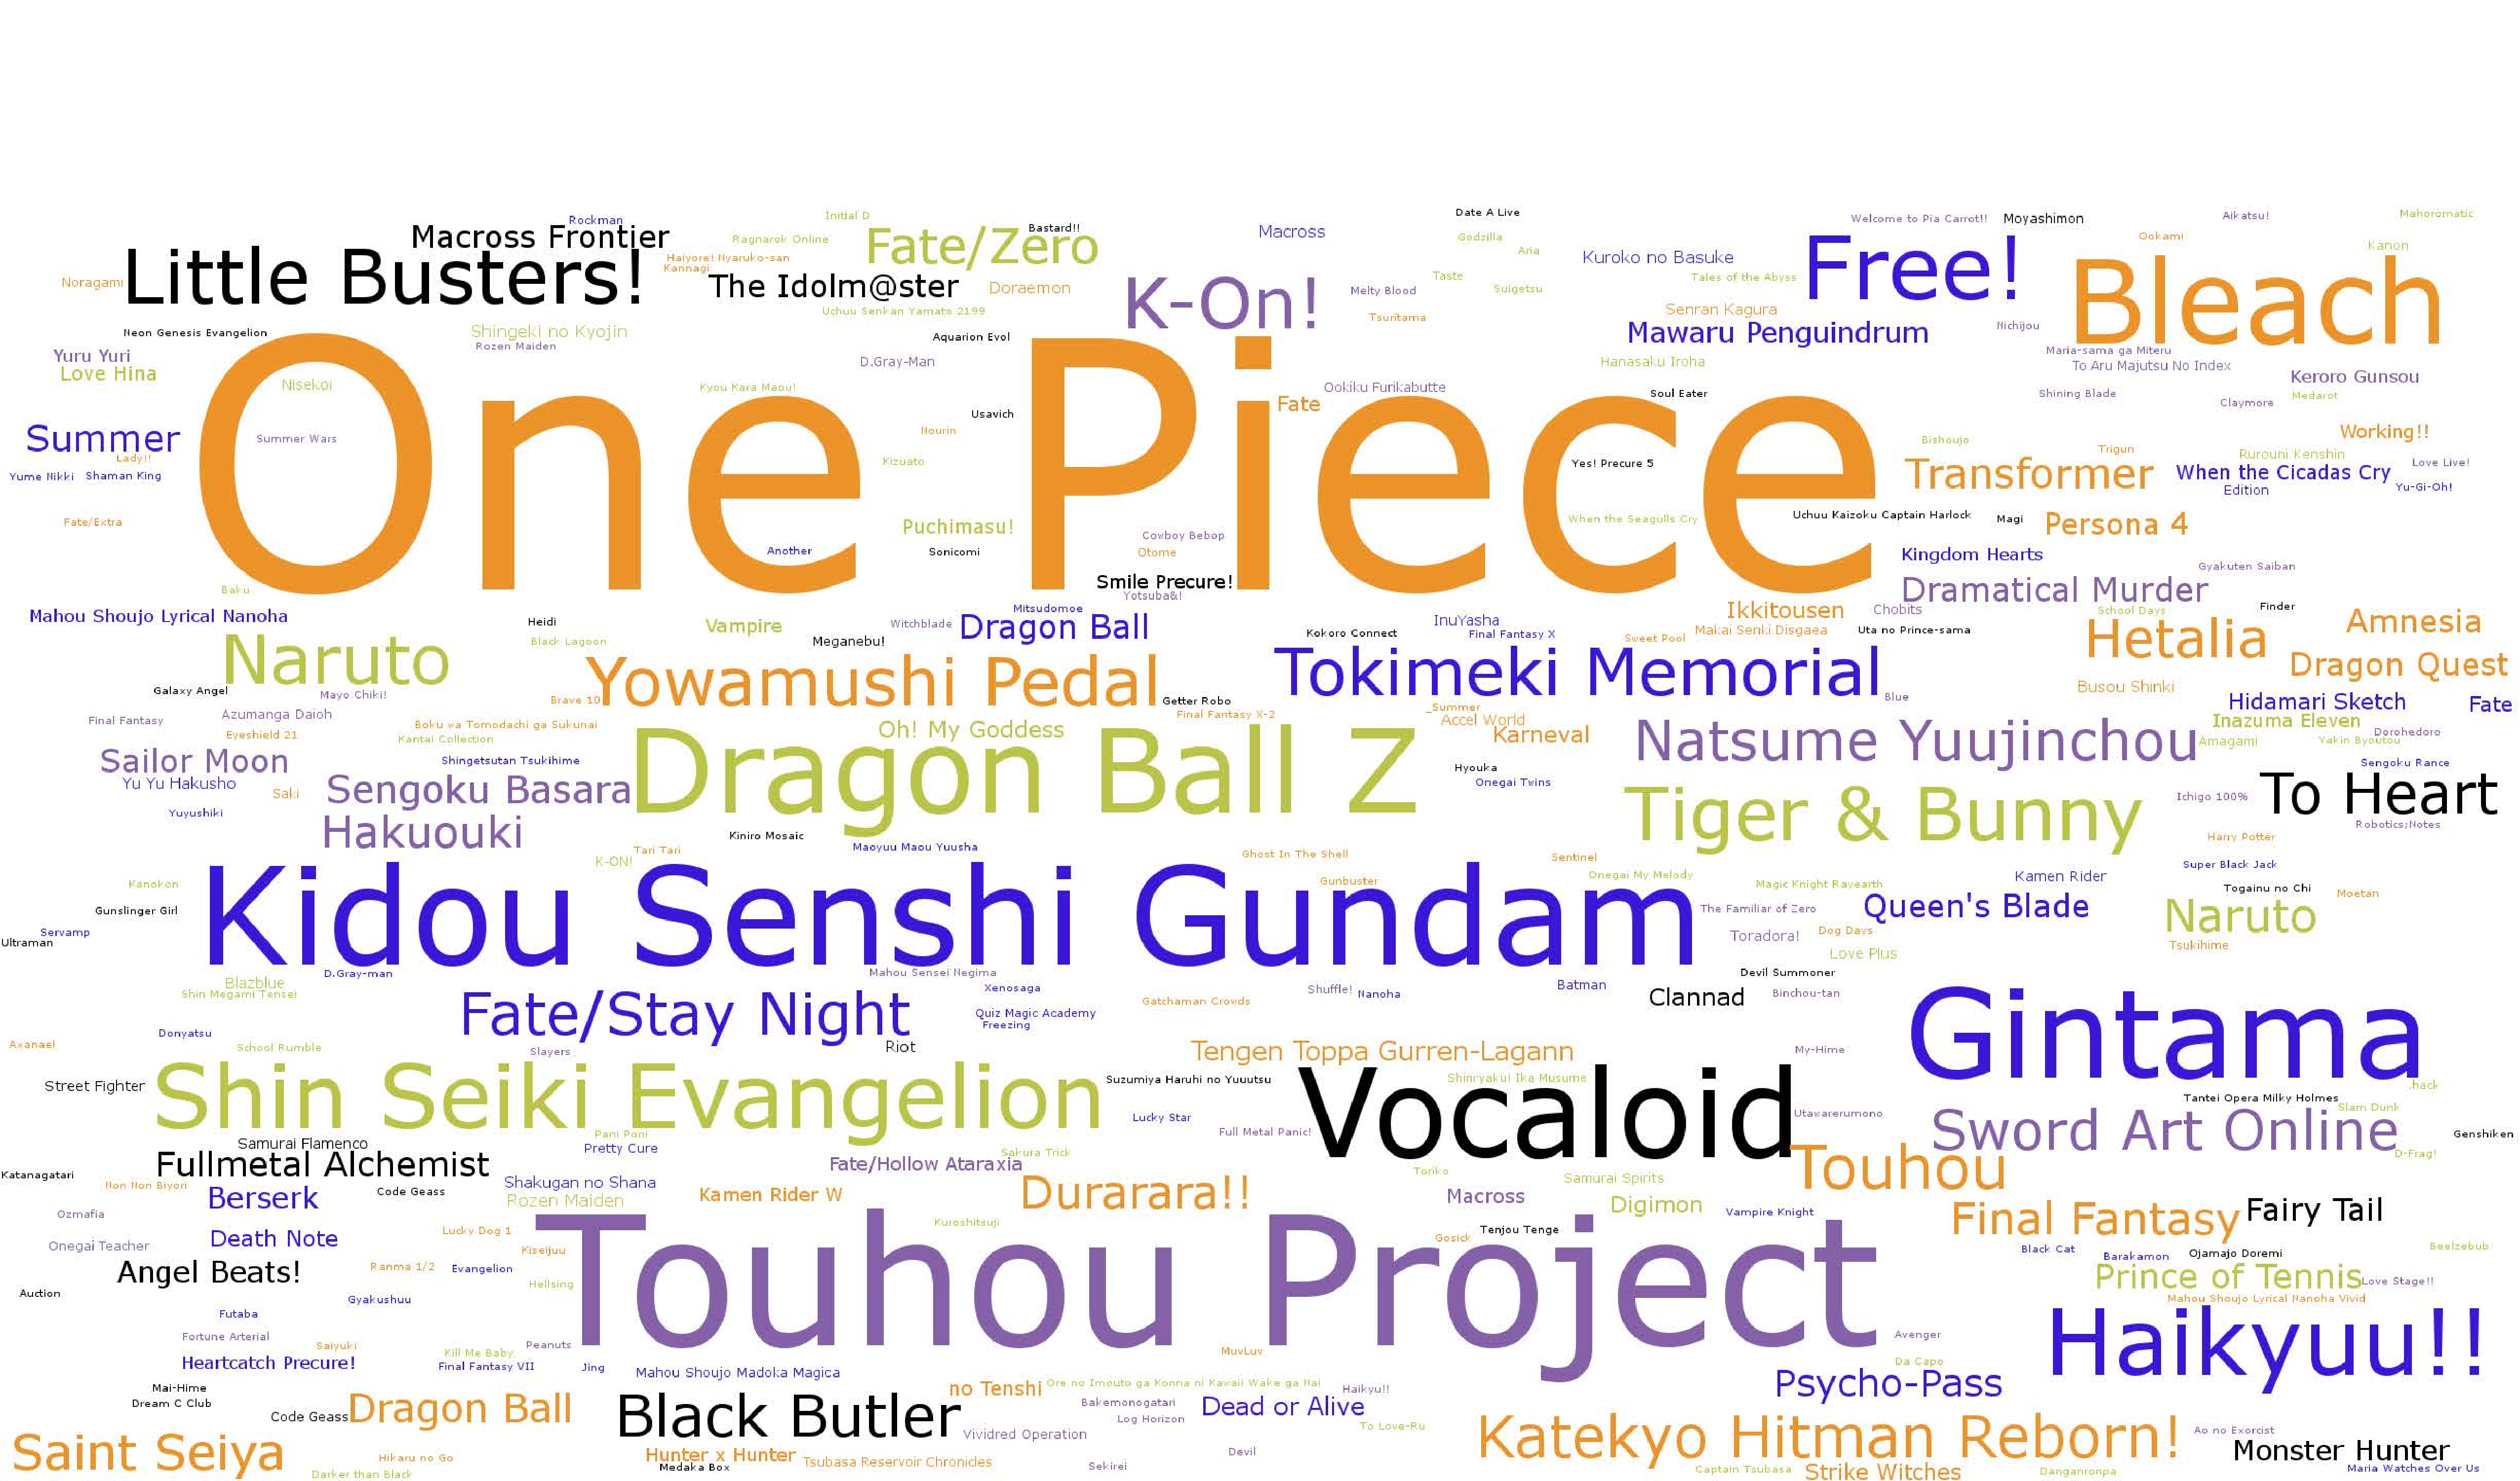
\includegraphics[width=1\textwidth]{collection_amount_words.pdf}
\caption{Visualização de dados em nuvem de palavras. A imagem ilustra a quantidade de itens em cada franquia.} \label{collaborator}
\end{figure}

\begin{figure}[H]
\centering
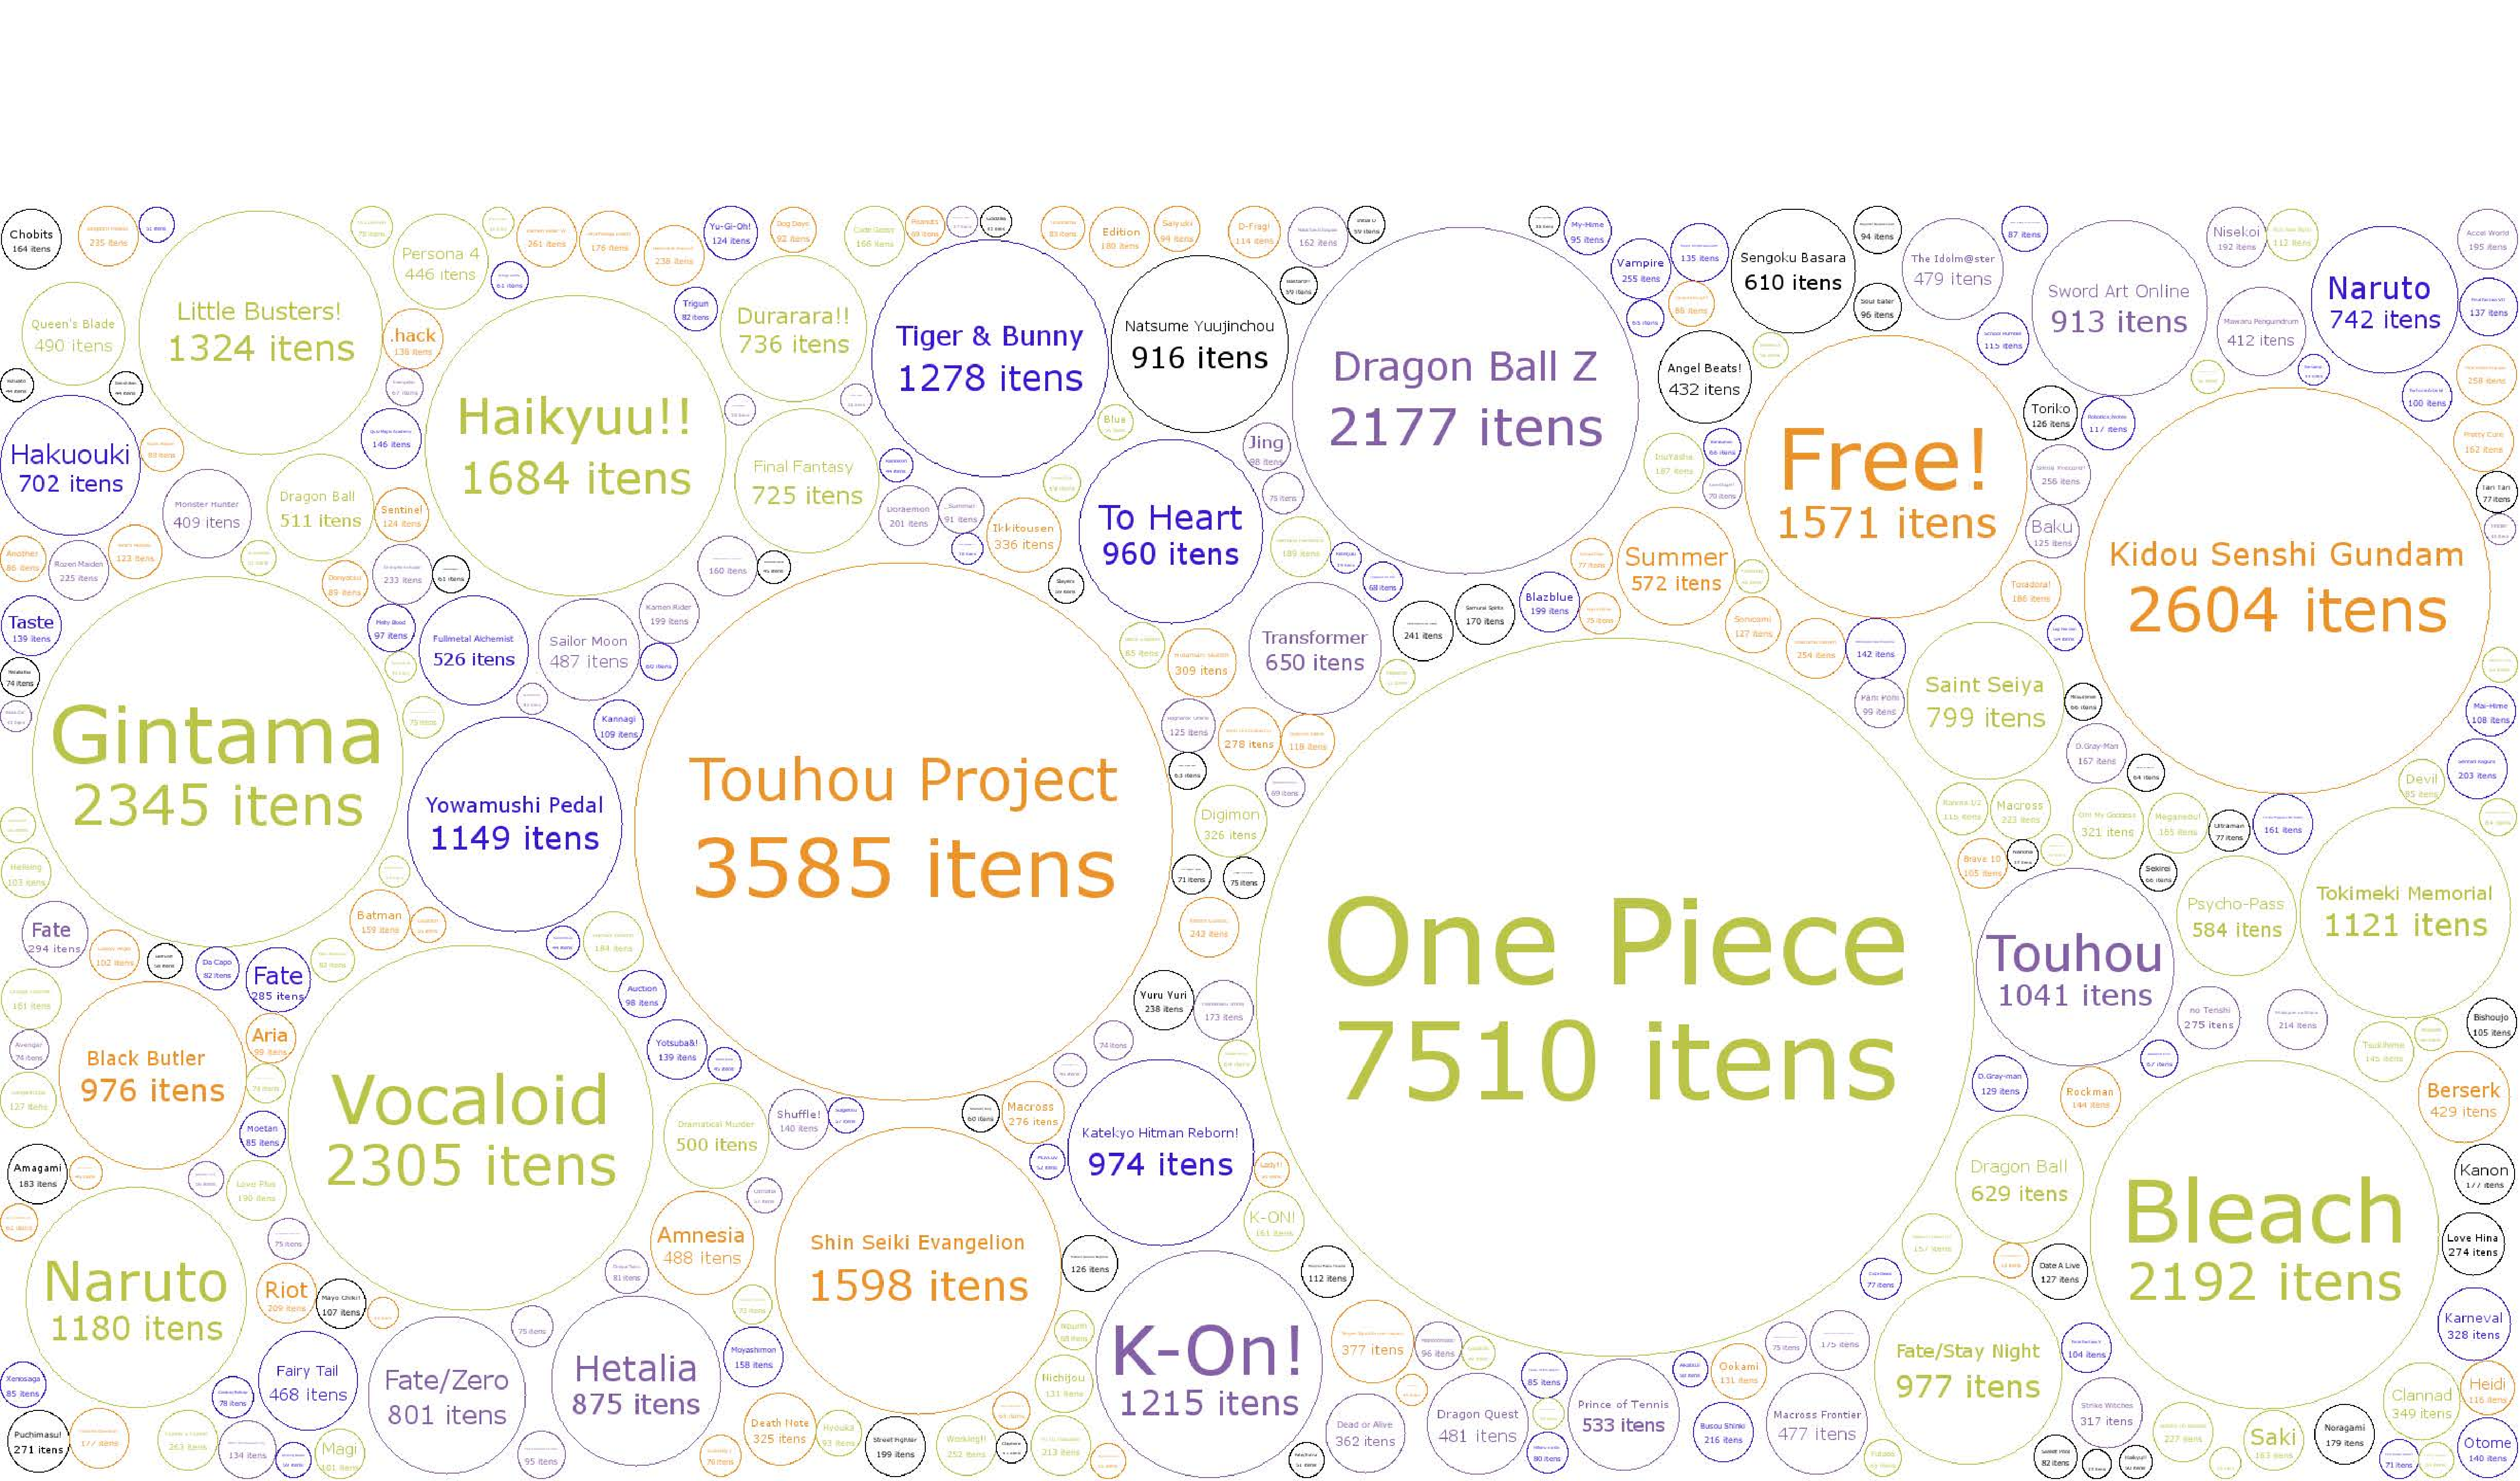
\includegraphics[width=1\textwidth]{collection_amount_bubbles.pdf}
\caption{Visualização de dados em nuvem de bolhas. A imagem ilustra a quantidade de itens em cada franquia.} \label{collaborator}
\end{figure}

\begin{figure}[H]
\centering
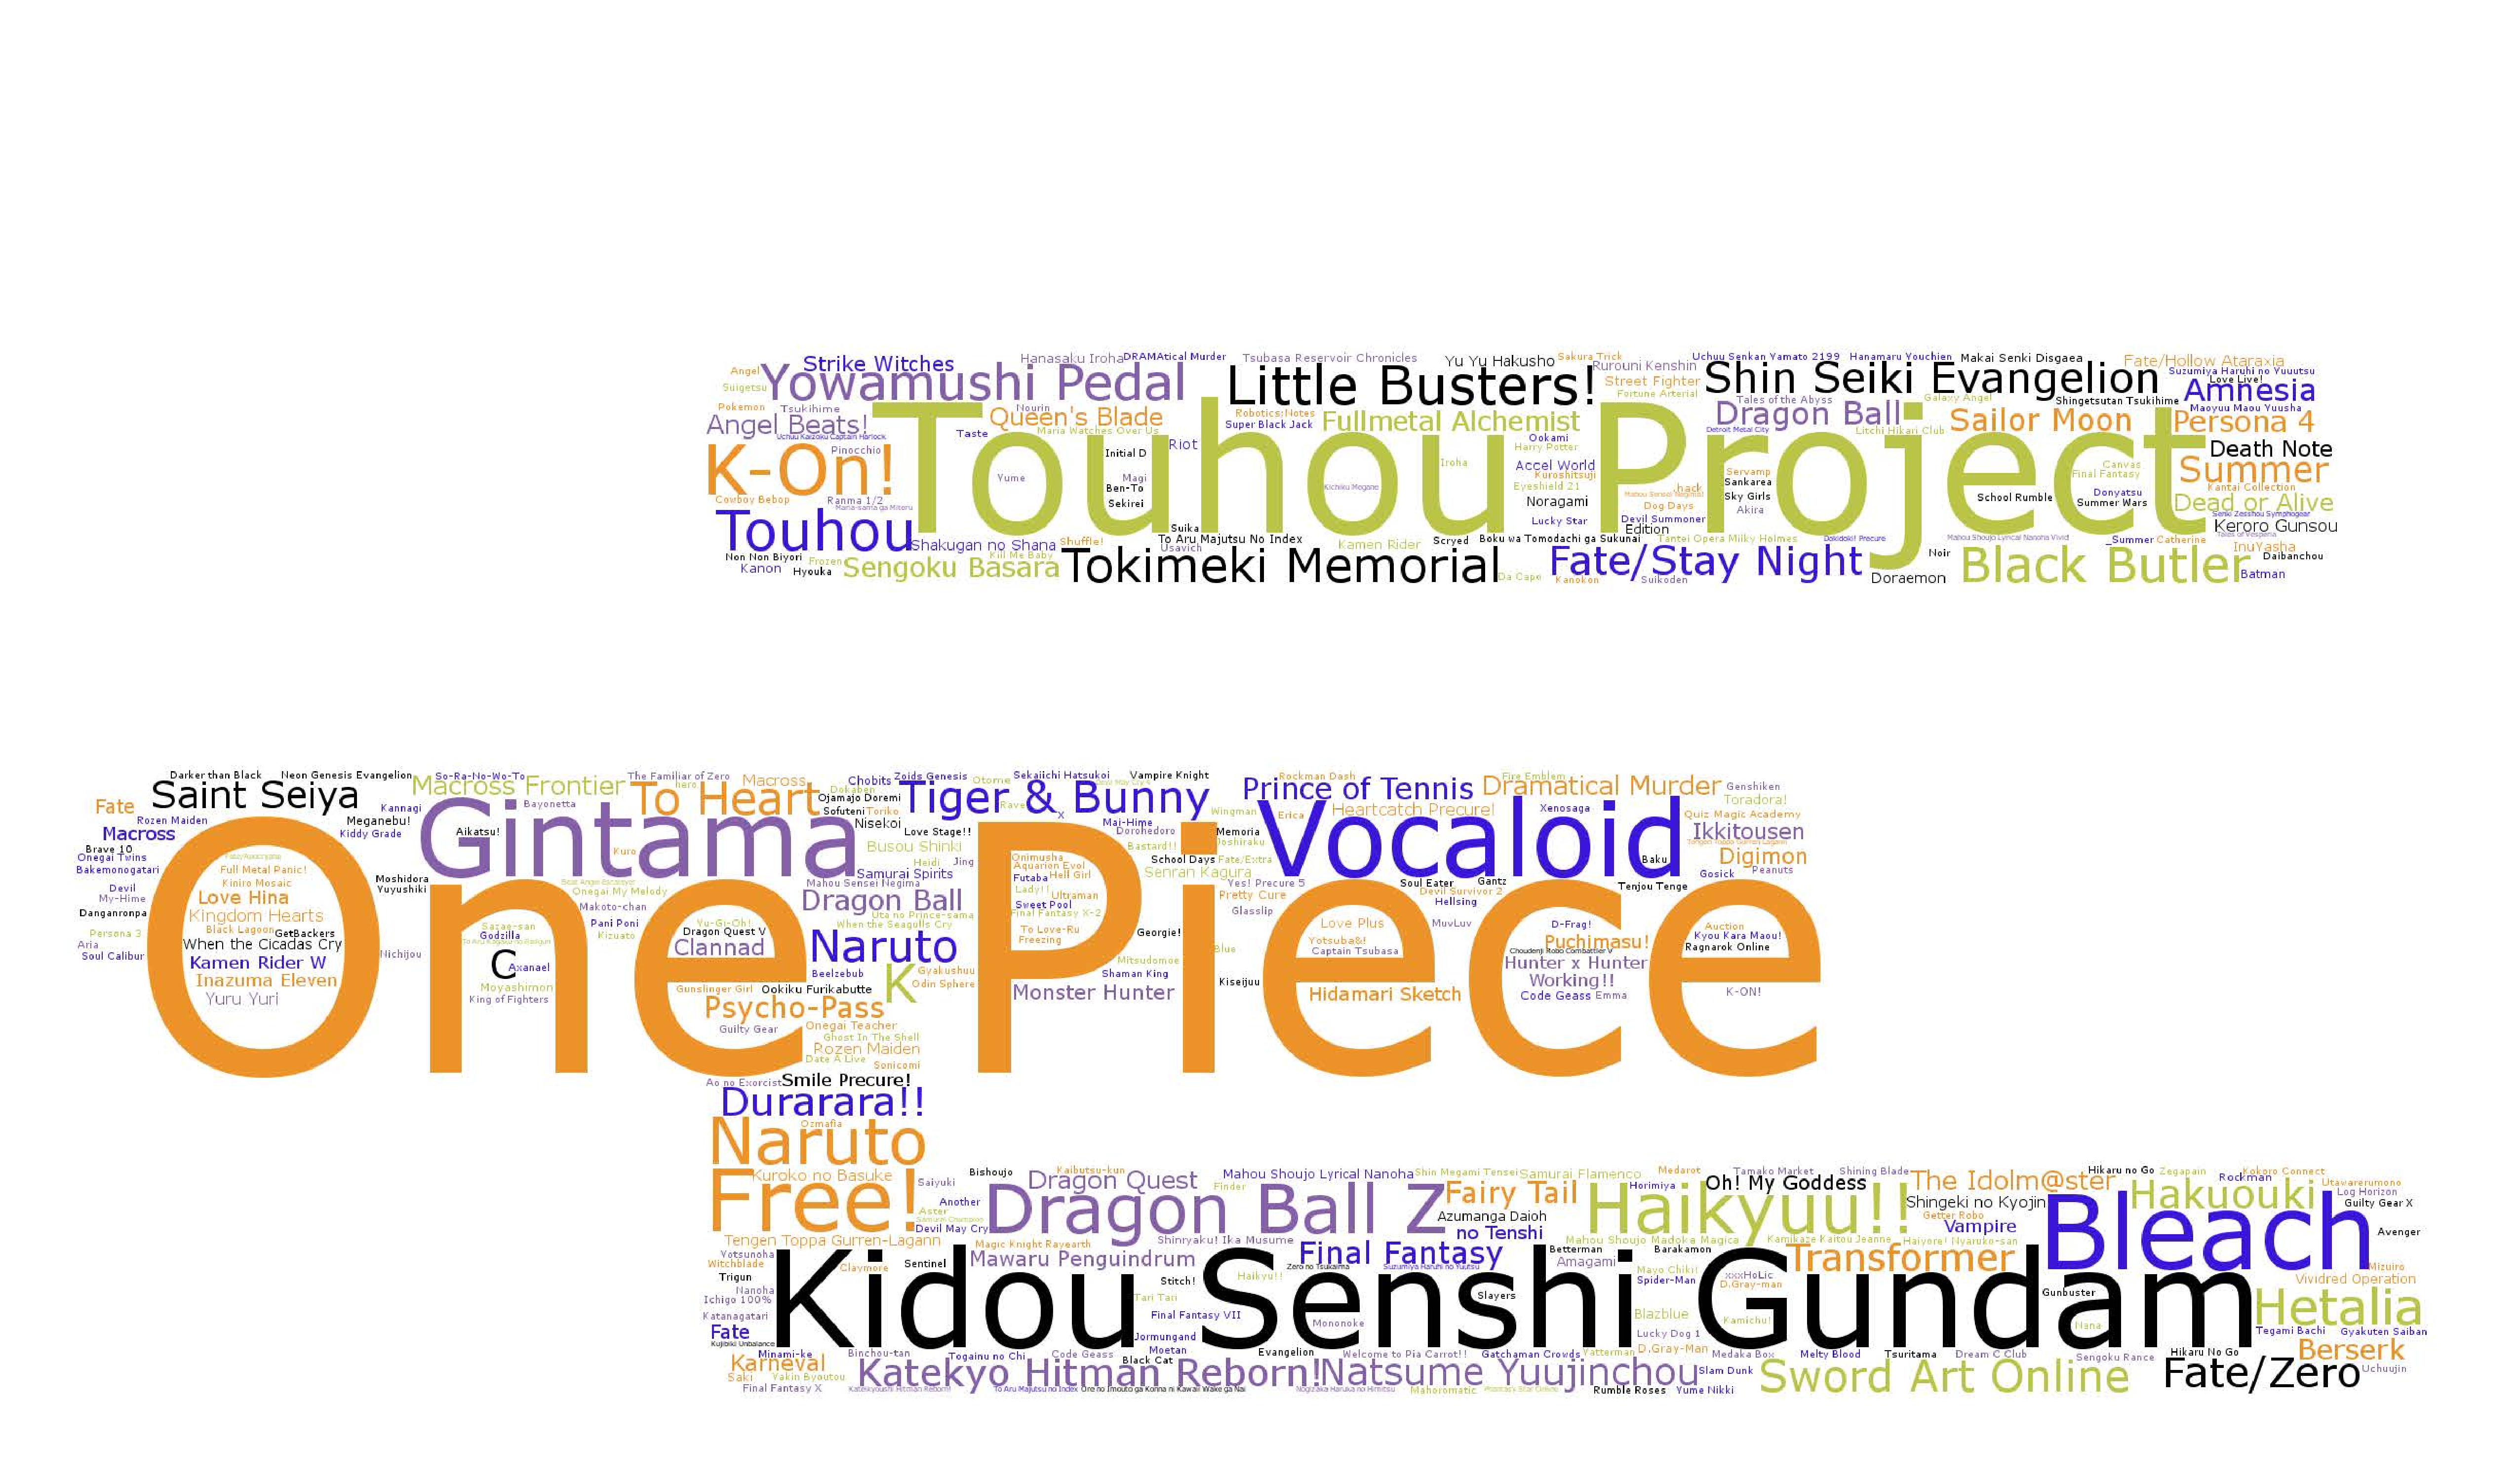
\includegraphics[width=1\textwidth]{collection_amount_mask.pdf}
\caption{Visualização de dados em nuvem de palavras com máscara. A imagem ilustra a quantidade de itens em cada franquia.} \label{collaborator}
\end{figure}

Para ambos os modelos o tempo de processamento é similar, e dependendo da quantidade de objetos (palavras ou círculos), a serem utilizados, podem ser processados em alguns minutos, em casos com 10 objetos, ou em 24 horas, em casos com 3.000 objetos. A maior parte do tempo é consumida pela busca por espaço disponível.

\bibliographystyle{plain}
\begin{thebibliography}{2}

%
\bibitem{integral}
{P. Viola; M. Jones.}
\newblock {\emph{Rapid object detection using a boosted cascade of simple
features}. In IEEE Computer Vision and Pattern Recognition (pp. I:511–518), 2001.}

\bibitem{representation}
{Konstantinos G. Derpanis.}
\newblock {\emph{Integral image-based representations}, Department of Computer Science and Engineering, York University, New York, 2007.}

\bibitem{lang}
{Marco Lui; Timothy Baldwin.}
\newblock {\emph{langid.py: An Off-the-shelf Language Identification Tool}, Department of Computing and Information Systems, University of Melbourne, VIC 3010, Australia.}

\bibitem{tutorial} Scrapy developers. \emph{Scrapy Tutorial}, 2014, disponível em \url{http://doc.scrapy.org/en/latest/intro/tutorial.html}.

\bibitem{tutorial} Fredrik Lundh. \emph{The Python Imaging Library Handbook}, 2014, disponível em \url{http://effbot.org/imagingbook/}.

\end{thebibliography}
\end{document}